\documentclass{article}

\usepackage[utf8]{inputenc}
\usepackage{graphicx}
\usepackage{hyperref}
\usepackage{float} % Carga el paquete float
\usepackage{tikz}
\usepackage[margin=1in]{geometry}


\usetikzlibrary{positioning}
\usepackage[left=0.6in, right=0.6in]{geometry}

\title{\textit{History of War}}
\author{Carpintero Díaz David, Seijo García Pablo}
\date{\today}

\begin{document}

\maketitle
\tableofcontents
\newpage

\section{History of War: Un camino por la historia}

Nuestra página web está dedicada a la historia bélica del mundo. La página web cuenta con diferentes secciones con información variada.
La sección más llamativa es un mapa interactivo que sirve como portal a las páginas de las batallas más significativas de todas las épocas. Este mapa permite explorar visualmente el desarrollo de conflictos, desde las antiguas guerras hasta los enfrentamientos contemporáneos, brindando una perspectiva única y global de la historia militar.

También cuenta con diversos apartados temáticos, donde se encuentra información detallada sobre guerras que han moldeado naciones enteras, batallas que han cambiado el curso de la historia y personajes legendarios cuyas acciones resonaron a lo largo del tiempo. Cada sección está cuidadosamente elaborada para ofrecer datos exhaustivos y análisis profundos, proporcionando un contexto completo para comprender el trasfondo y la importancia de cada acontecimiento.

Además contamos con una biblioteca, que cuenta con una selección de libros recomendados, cada uno abordando distintas épocas de la historia bélica con profundidad. Cada recomendación va acompañada de una breve pero informativa descripción, que te brindará una visión general del contenido y del enfoque particular del libro.

\newpage

\section{Inventario de Contenido}

Con el objetivo de establecer una estructura clara y organizada para el desarrollo de nuestra página web, hemos procedido a la elaboración de un inventario de contenido. Dicho inventario actúa como un esquema preliminar que facilitará la implementación final del sitio web.

\begin{figure}[H]
    \centering
    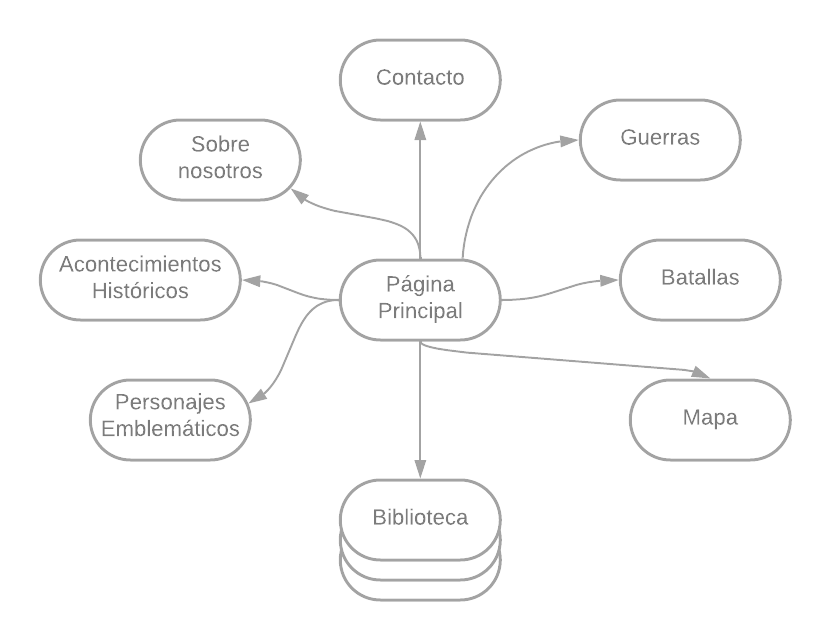
\includegraphics[width=0.6\textwidth]{Esquemas/InventarioContenido.png}
    \caption{Inventario de Contenido}
    \label{fig:mi_imagen}
\end{figure}

Nuestra plataforma se articula en diversas secciones, cada una con un propósito específico y contenido diferenciado. De particular relevancia es la sección denominada "Biblioteca", la cual albergará una selección cuidadosamente curada de libros recomendados. Asimismo, destacamos la inclusión de un mapa interactivo, diseñado para guiar a los usuarios a través de diversos episodios históricos, permitiéndoles explorar las distintas batallas que han marcado el curso del tiempo. Adicionalmente, la sección dedicada a las guerras ofrecerá una visión exhaustiva sobre los múltiples conflictos bélicos que han tenido lugar a lo largo de la historia, proporcionando información detallada y contextos relevantes.

\newpage

\section{Arquitectura de la Información}

Basándonos en el esquema preliminar previamente delineado, procedemos a desarrollar la arquitectura de la información. Este proceso nos facilitará la organización de las ideas iniciales en una estructura jerárquica, la cual establecerá la profundidad y el alcance de cada sección dentro de nuestra página web.

\begin{figure}[H]
    \centering
    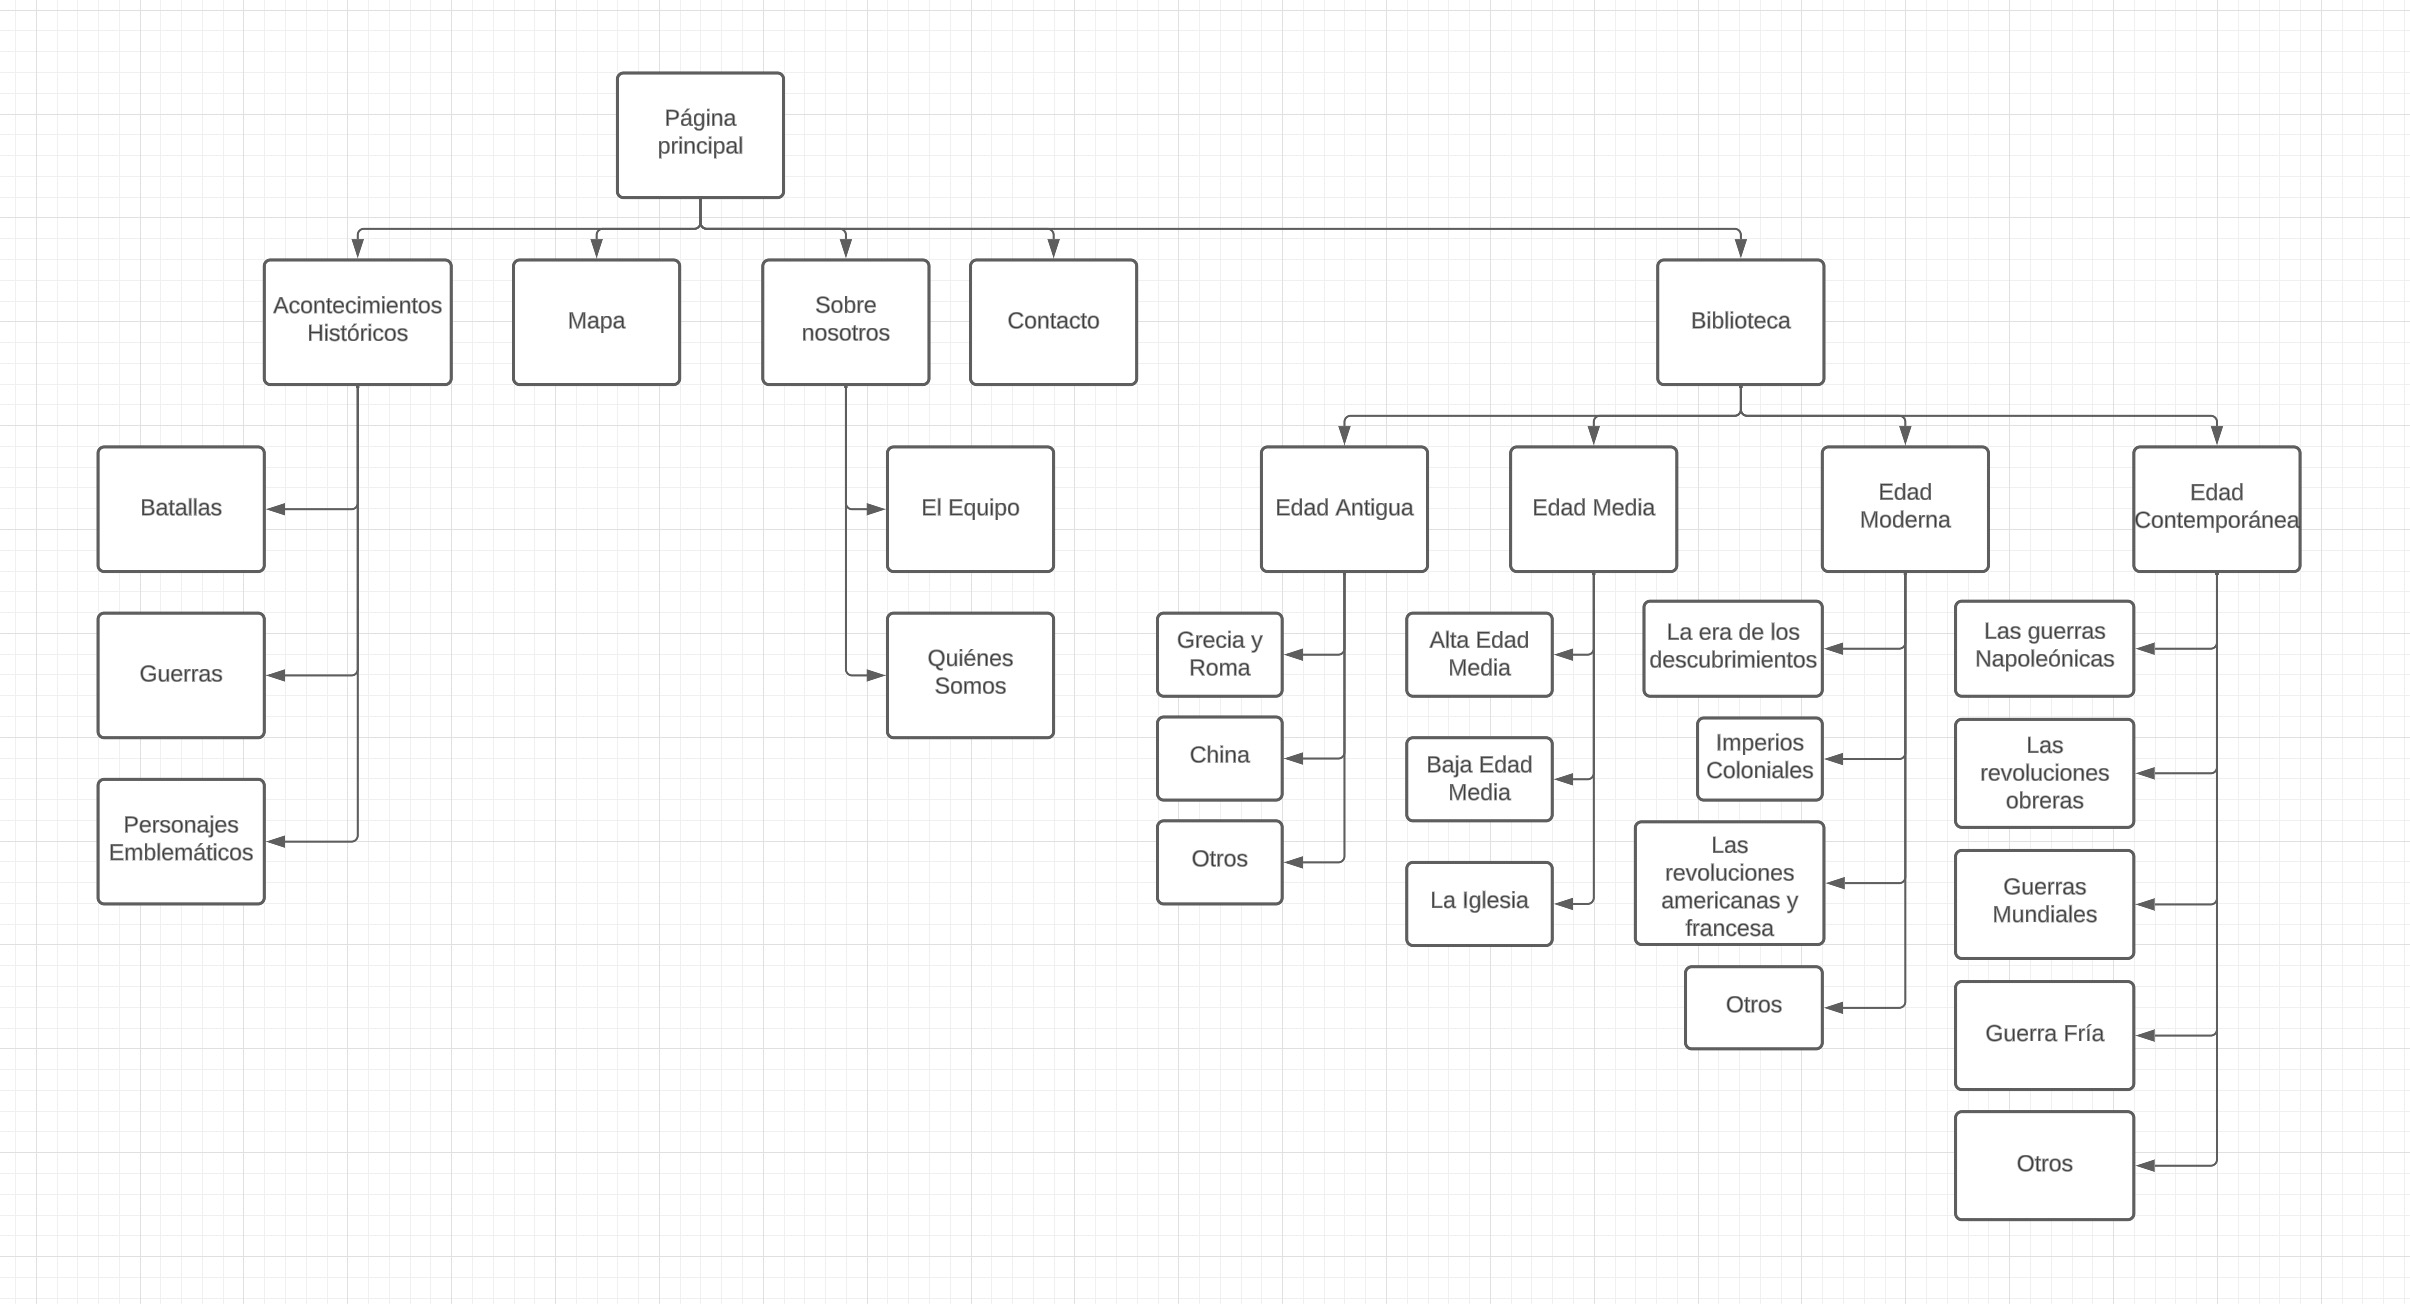
\includegraphics[width=1\textwidth]{Esquemas/Arquitectura de Informacion.jpg}
    \caption{Arquitectura de la Información}
    \label{fig:mi_imagen}
\end{figure}

Dentro de esta arquitectura, la sección más amplia corresponde a la biblioteca. Esta área está meticulosamente segmentada en diversas subsecciones que reflejan las distintas eras históricas, abarcando desde la Edad Antigua, iniciando en el año 3000 a.C., hasta la contemporaneidad. Esta organización no solo facilita la navegación sino que también enriquece la experiencia educativa del usuario al proporcionar un contexto histórico claro y bien definido.

Adicionalmente, cabe resaltar la sección denominada "Acontecimientos Históricos", la cual funciona como categoría principal para temas relacionados con guerras, batallas y figuras históricas destacadas. Esta categorización permite una exploración temática coherente y detallada de los eventos que han moldeado la historia humana.

En conjunto, la arquitectura de la información diseñada busca optimizar la usabilidad y accesibilidad del sitio web, asegurando que los usuarios puedan navegar de manera intuitiva y obtener información de forma eficiente.

\newpage

\section{Casos de Uso Típicos}

Tras definir la estructura de nuestro sitio web, presentaremos los casos de uso comunes, los cuales mostrarán las acciones que los usuarios pueden realizar al visitar nuestra página.

Esta parte es esencial para entender cómo los visitantes interactúan con el sitio, desde explorar las diferentes secciones hasta acceder a contenidos específicos. El objetivo es proporcionar una visión clara de lo que se espera que los usuarios hagan y cómo pueden aprovechar al máximo los recursos disponibles en la web.

\begin{figure}[H]
    \centering
    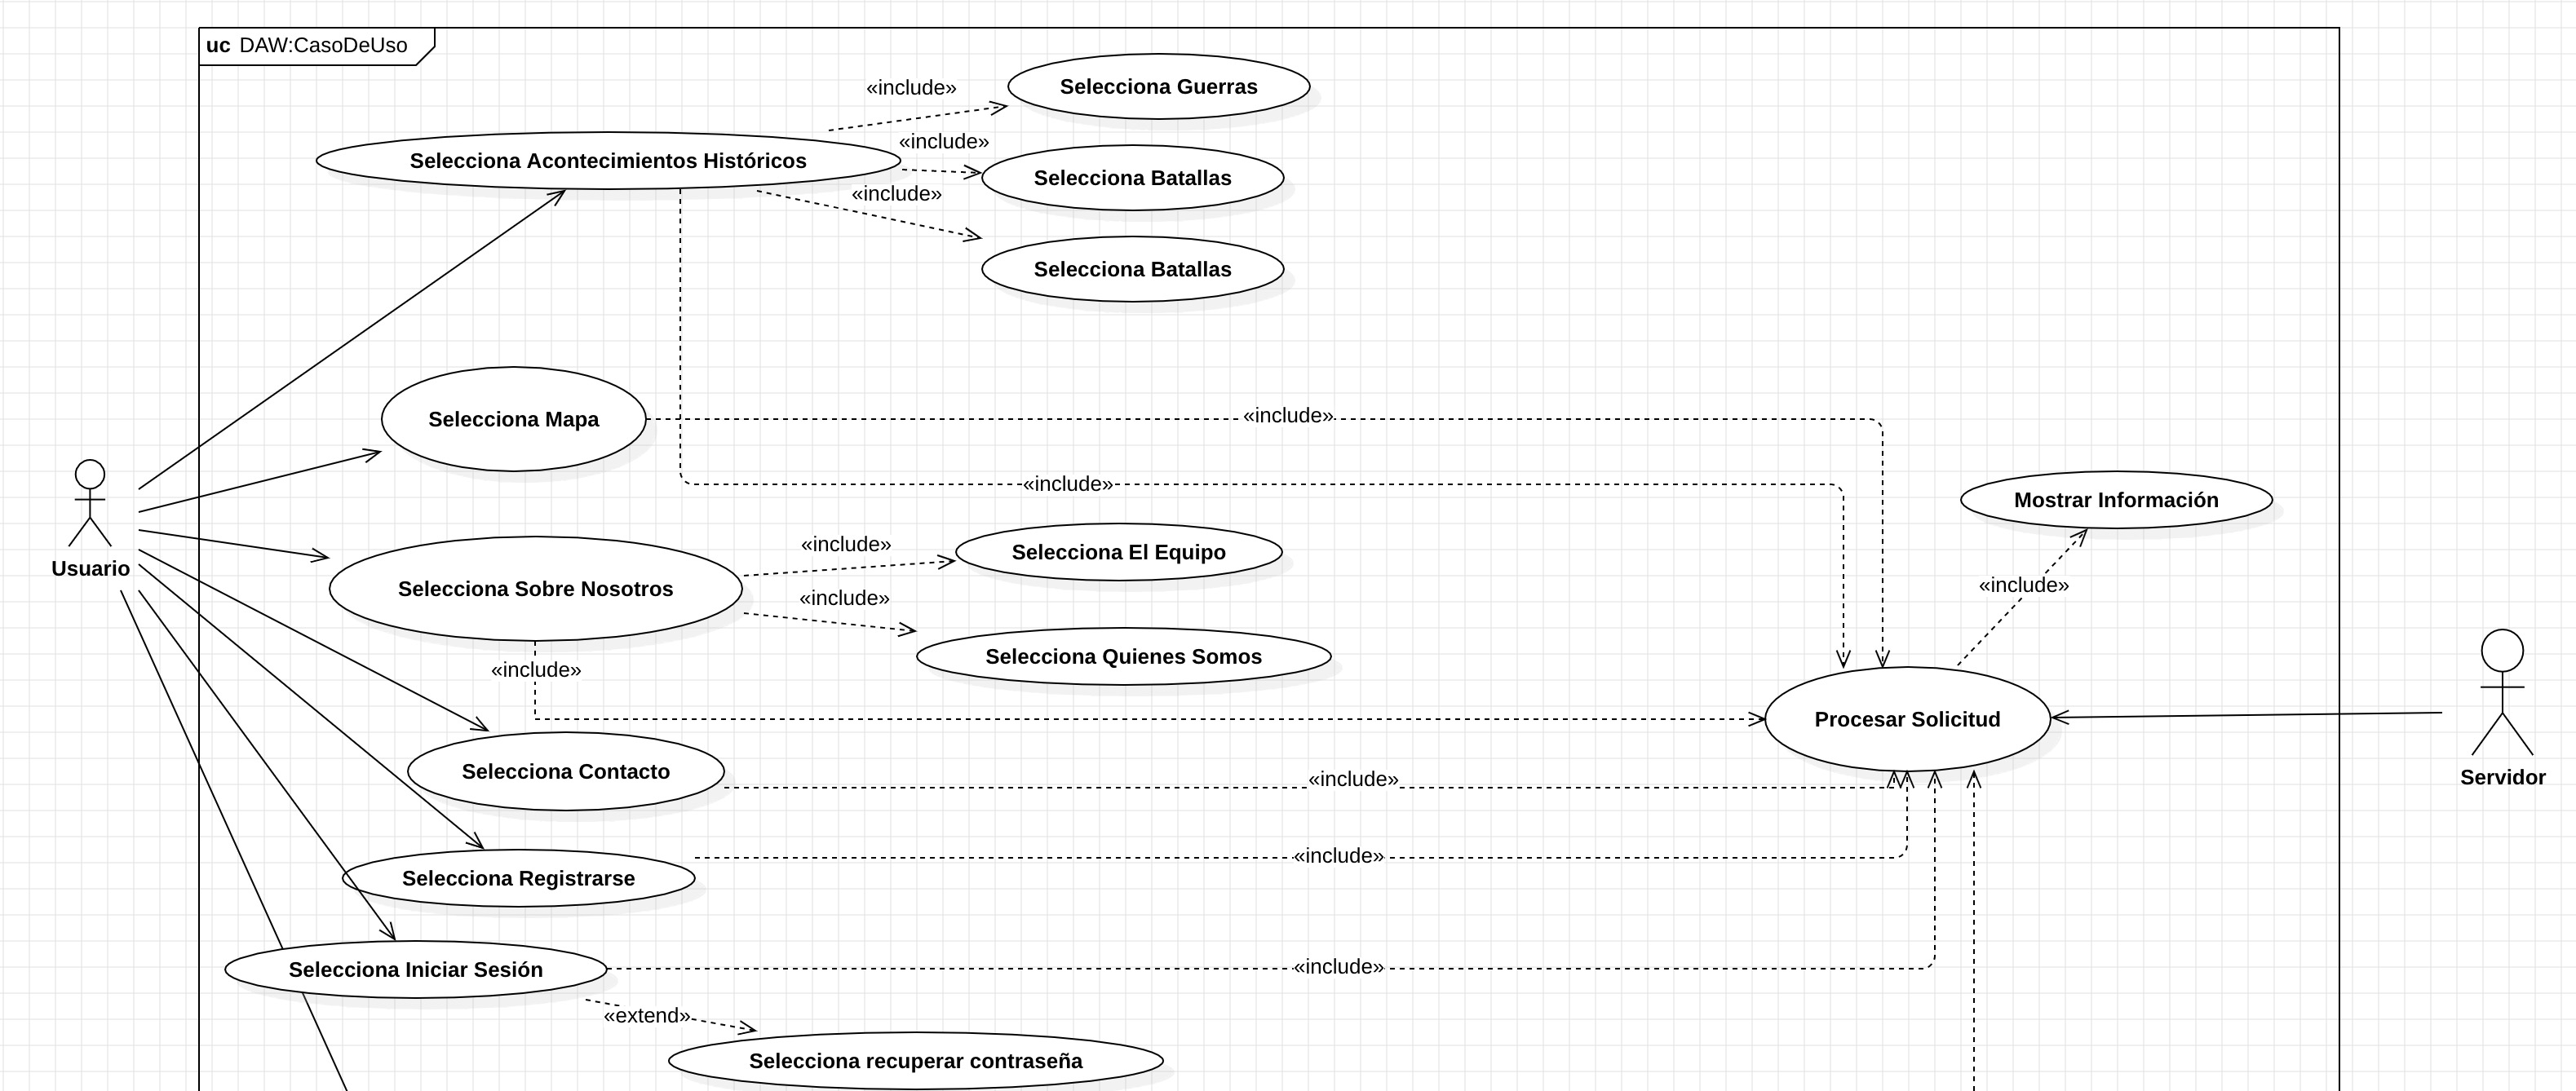
\includegraphics[width=1\textwidth]{Esquemas/CasosDeUsoSegmentado(1).jpg}
    \caption{Casos de Uso Típicos (1)}
    \label{fig:mi_imagen}
\end{figure}

\begin{figure}[H]
    \centering
    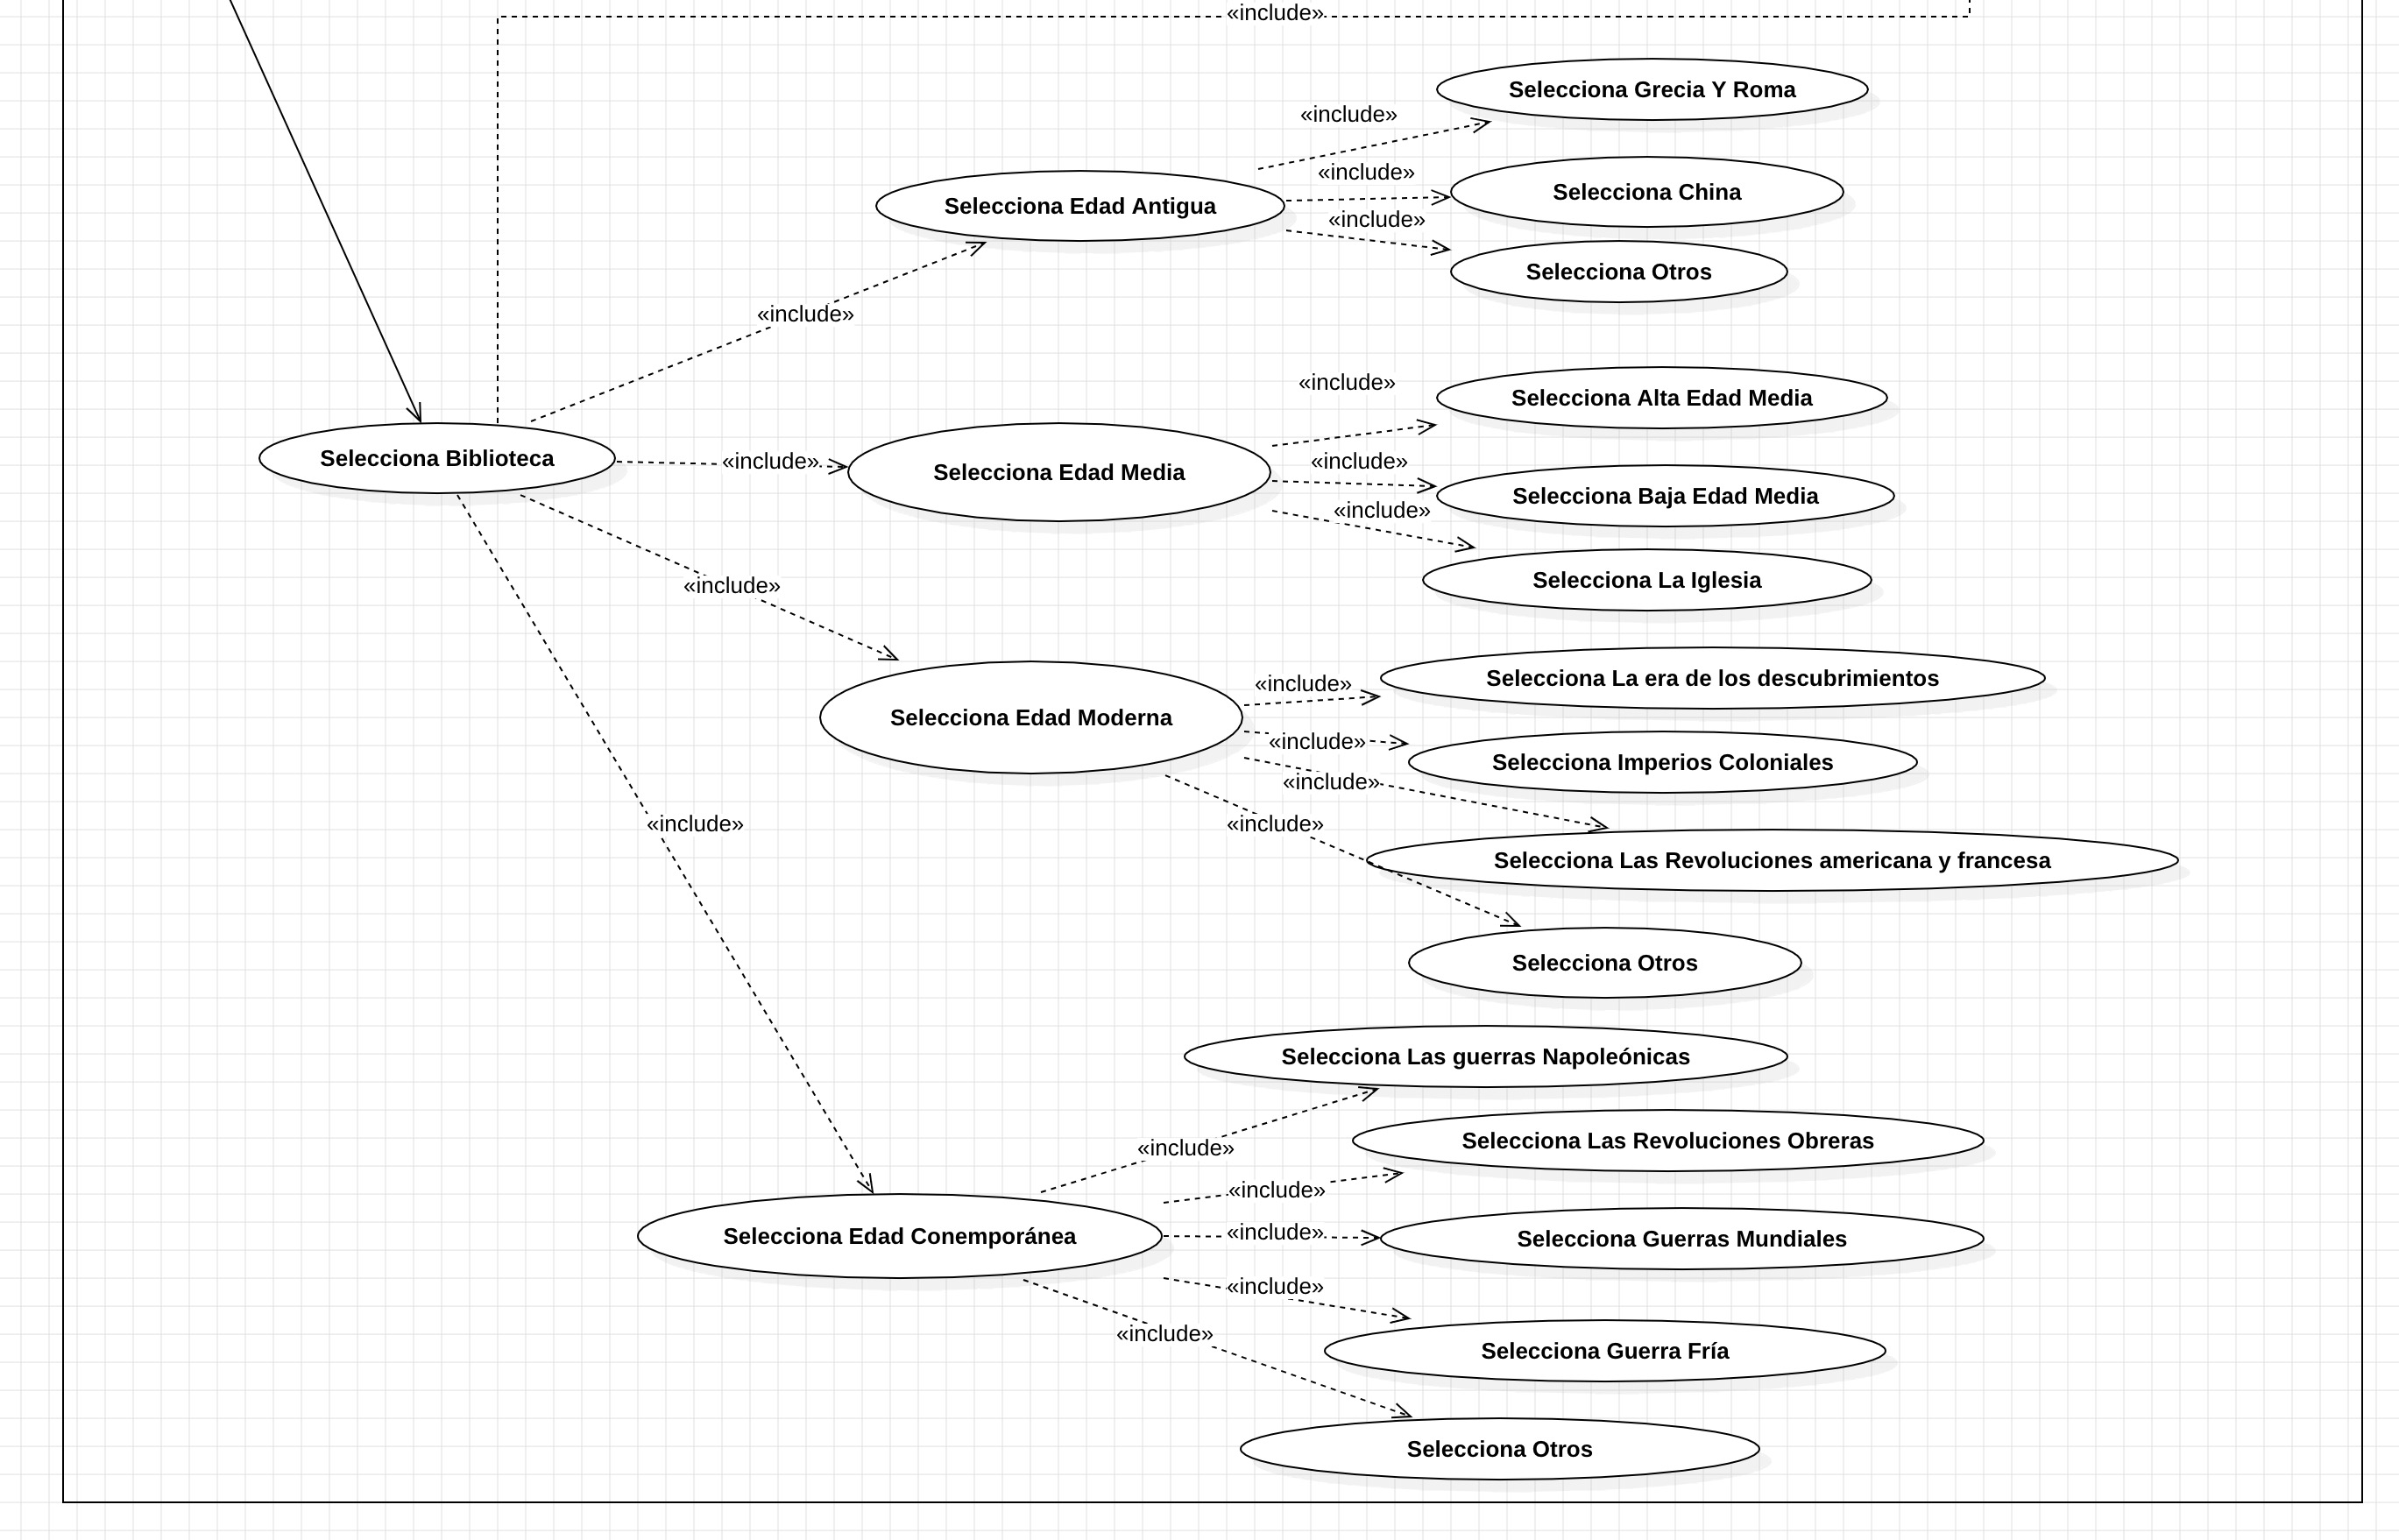
\includegraphics[width=1\textwidth]{Esquemas/CasosDeUsoSegamentado(2).jpg}
    \caption{Casos de Uso Típicos (2)}
    \label{fig:mi_imagen}
\end{figure}

\newpage

\section{Mapa de Navegación}

El mapa de navegación es un elemento clave en el diseño de nuestro sitio web, que actúa como una guía visual para estructurar y presentar la forma en que las distintas páginas y secciones están interconectadas. Este mapa facilita la comprensión de la organización del sitio, permitiendo a los usuarios y desarrolladores visualizar la jerarquía de la información y las rutas de acceso disponibles para navegar por el contenido. Al ofrecer una representación clara de cómo se organizan y relacionan los distintos componentes del sitio, el mapa de navegación mejora la usabilidad y la experiencia de usuario, asegurando que la información sea accesible y fácil de encontrar.

\begin{figure}[H]
    \centering
    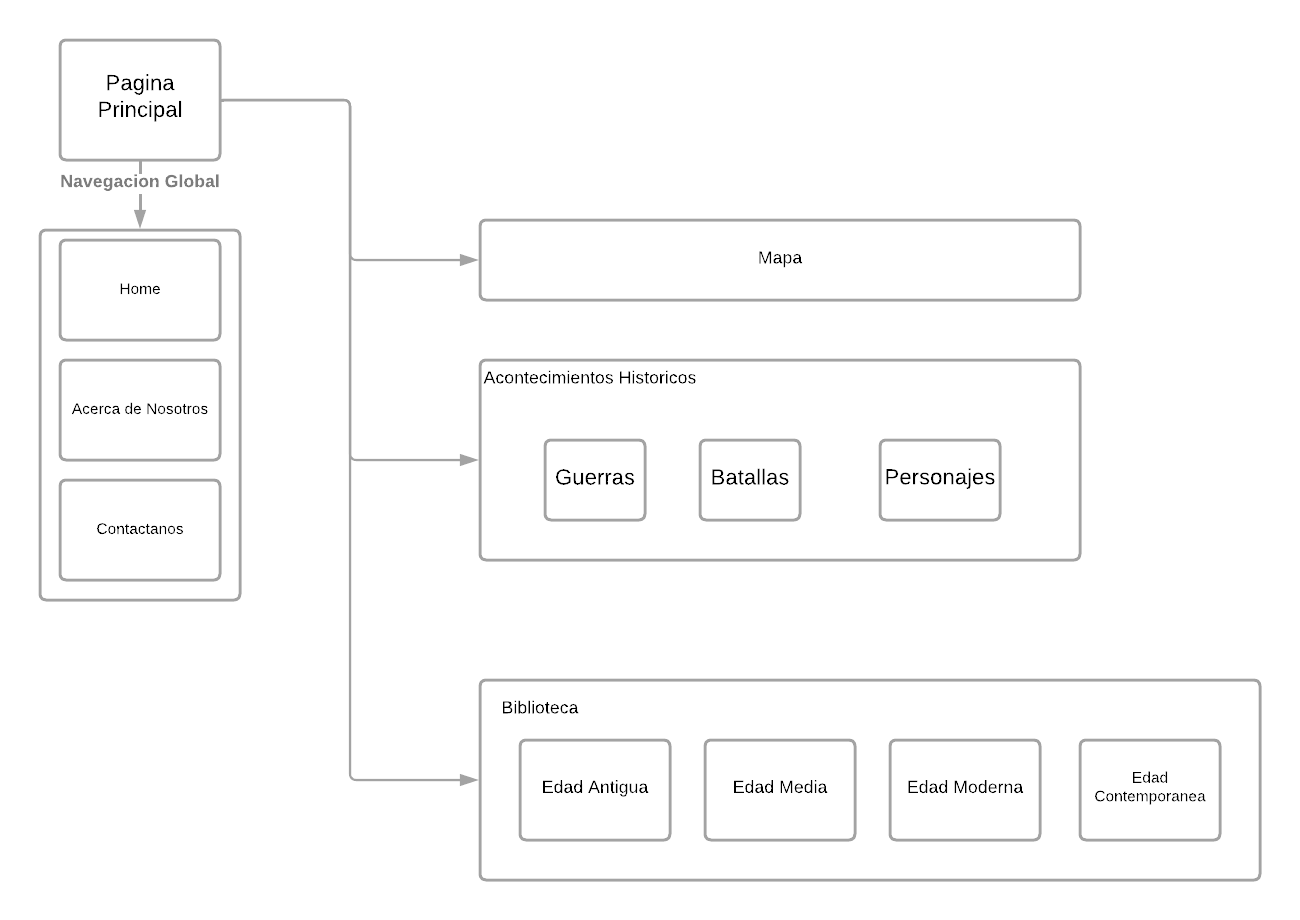
\includegraphics[width=1\textwidth]{Esquemas/MapawebFinal.png}
    \caption{Mapa de Navegación}
    \label{fig:mi_imagen}
\end{figure}

\newpage

\section{Interfaces}

\subsection{Manual (Boceto Manual)}

Se trata de un boceto manual de como nos imaginamos la página web, de tal manera que basaremos la evolución de la página basándonos en este concepto primigenio de las páginas.

\begin{figure}[H]
    \centering
    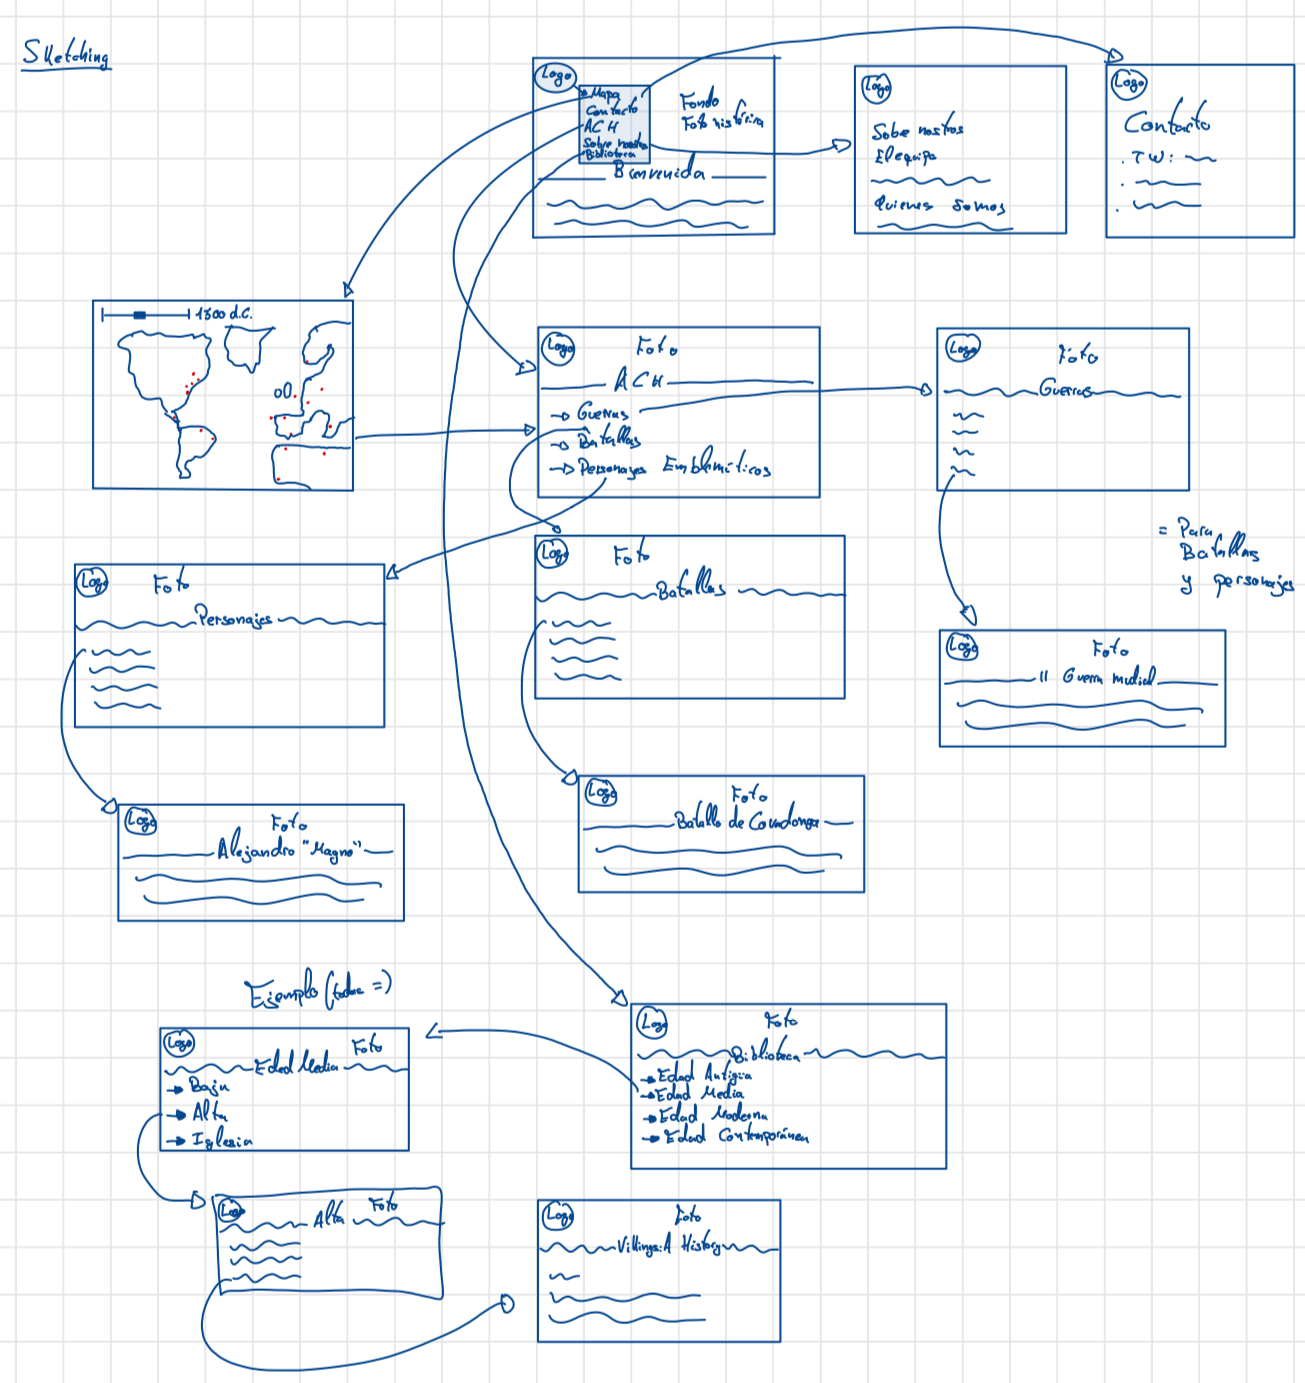
\includegraphics[width=1\textwidth]{Esquemas/Sketch.PNG}
    \caption{Boceto Manual}
    \label{fig:mi_imagen}
\end{figure}

\newpage

\subsection{Wireframes}

Los wireframes constituyen un conjunto de esquemas visuales que representan de forma preliminar el diseño y la estructura de nuestra página web. Estos bocetos iniciales son fundamentales para conceptualizar la disposición de los elementos en las páginas, sirviendo como base para el desarrollo y refinamiento posterior del sitio. A través de estos wireframes, establecemos un marco de referencia que guiará las fases subsiguientes del diseño, asegurando que la visión original se mantenga coherente a lo largo del proceso de desarrollo.

\begin{figure}[H]
    \centering
    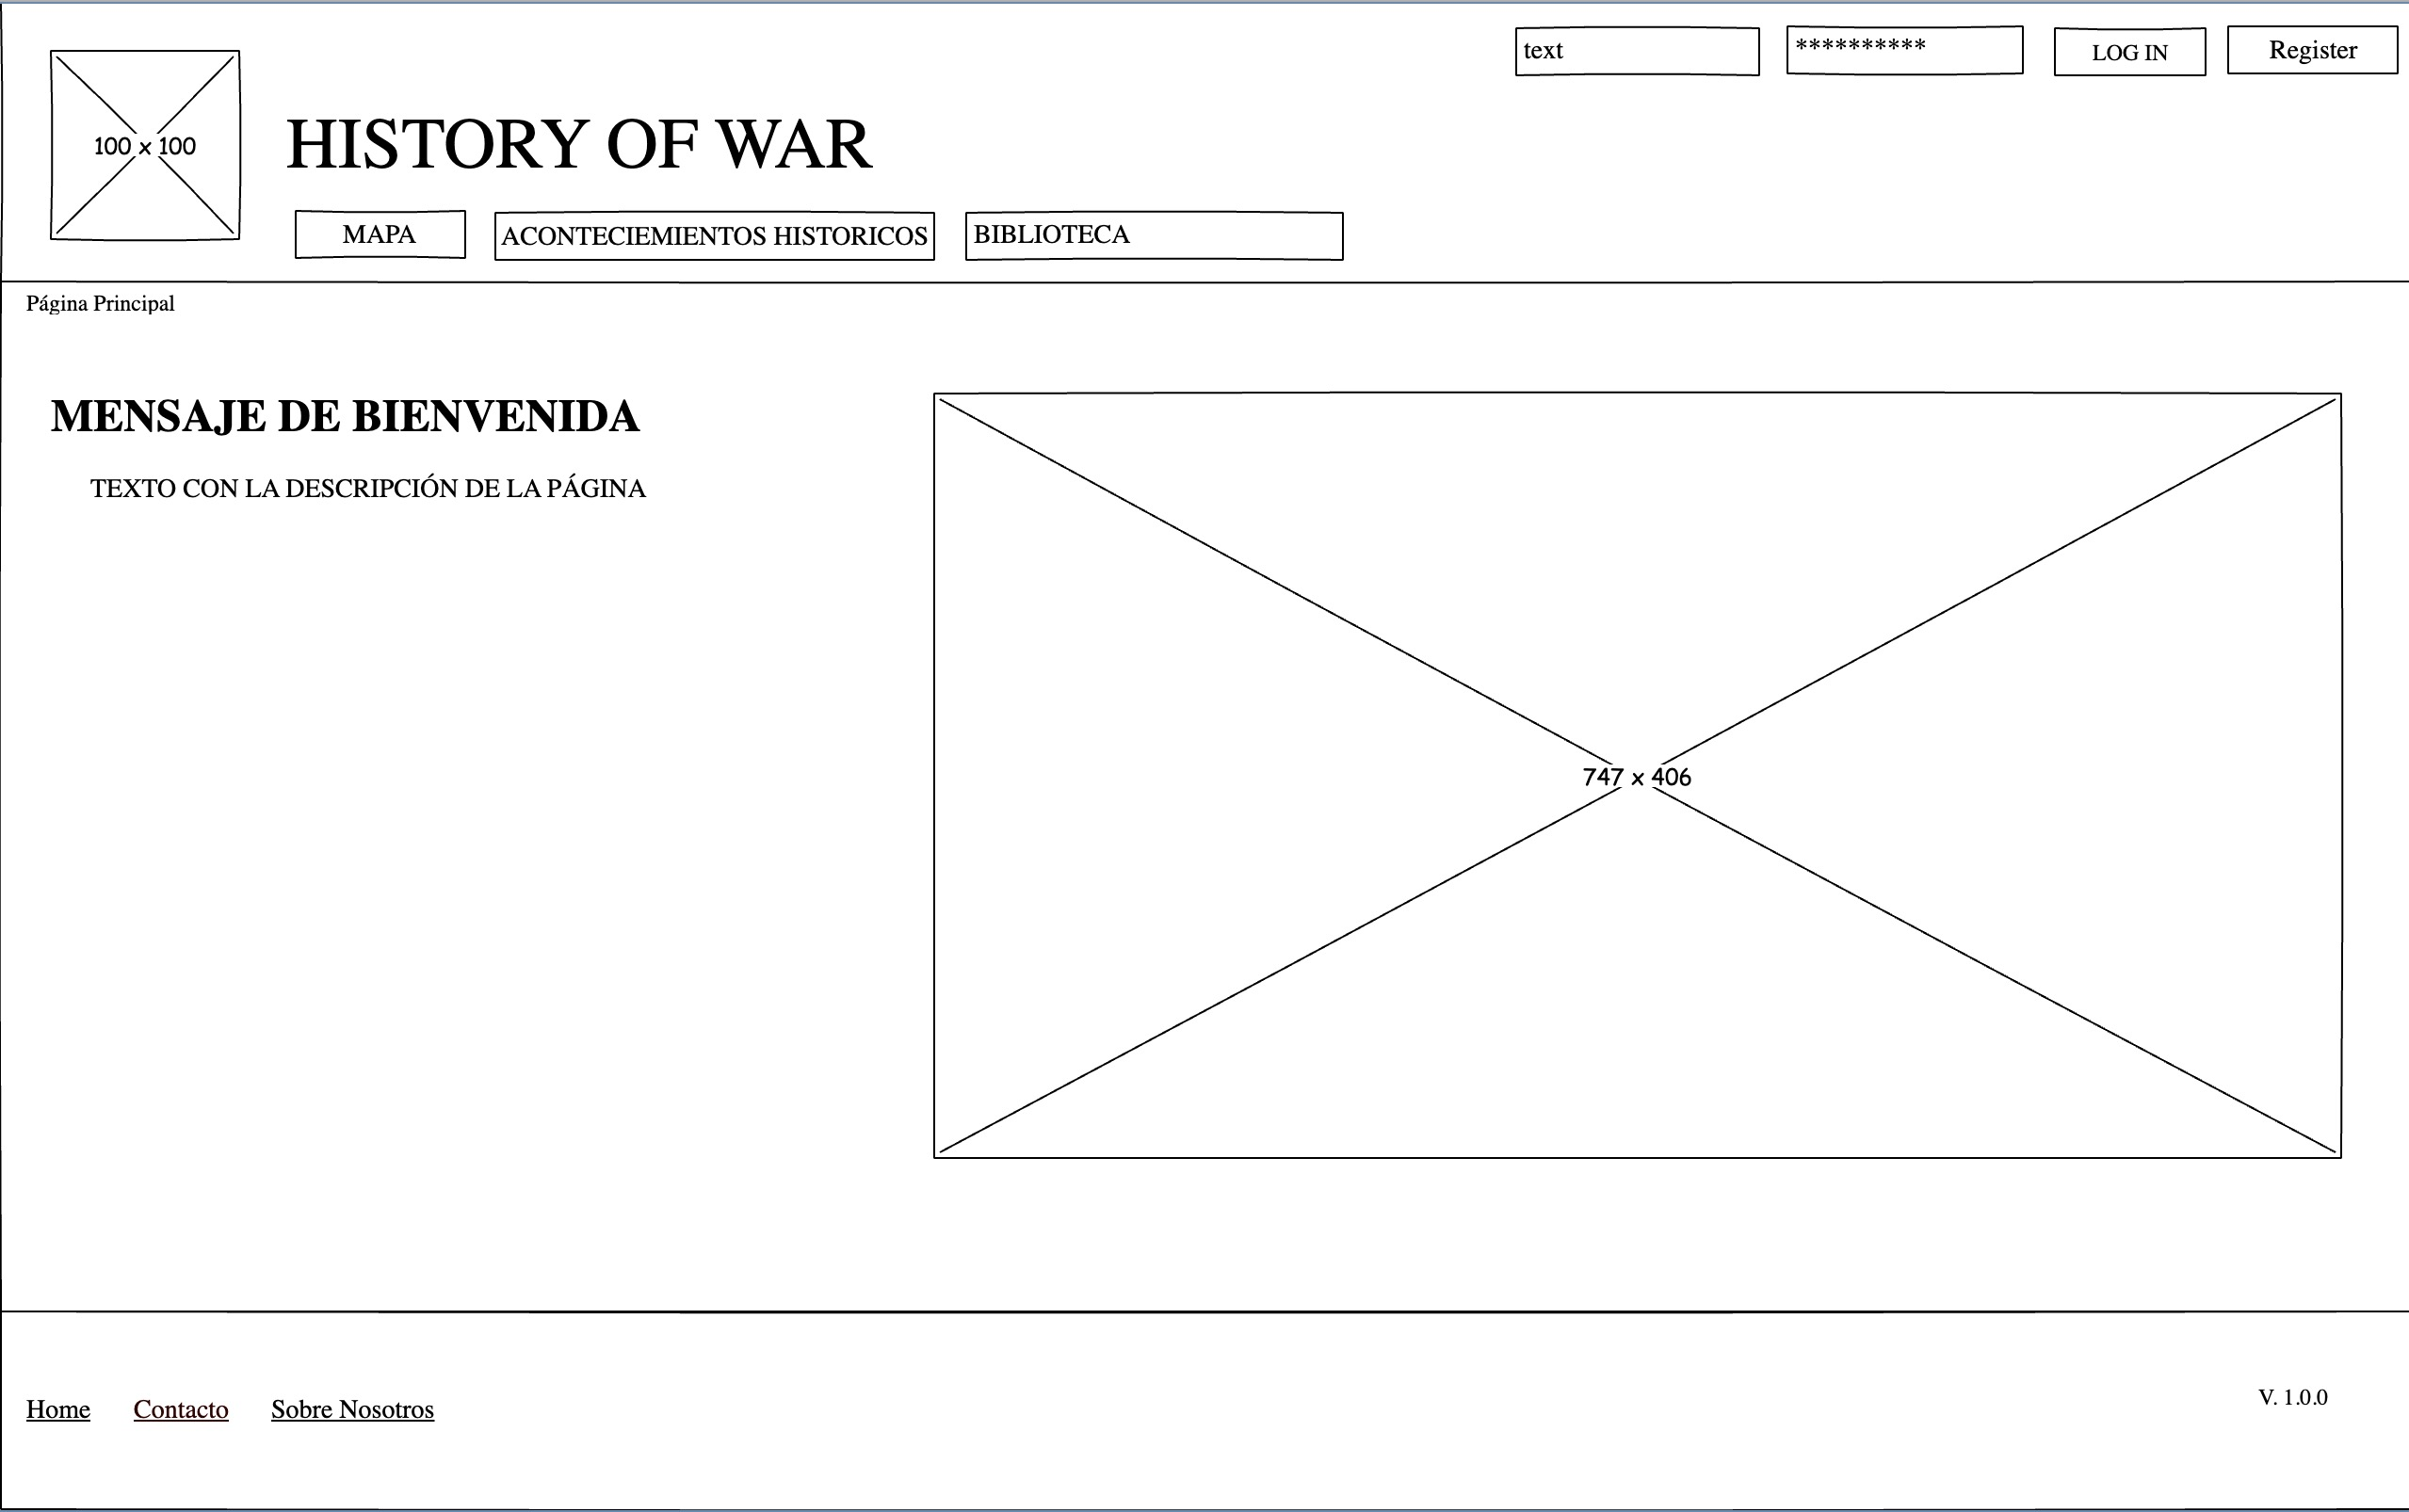
\includegraphics[width=1\textwidth]{Wireframes/PaginaPrincipal.jpg}
    \caption{Página Principal}
    \label{fig:mi_imagen}
\end{figure}

\begin{figure}[H]
    \centering
    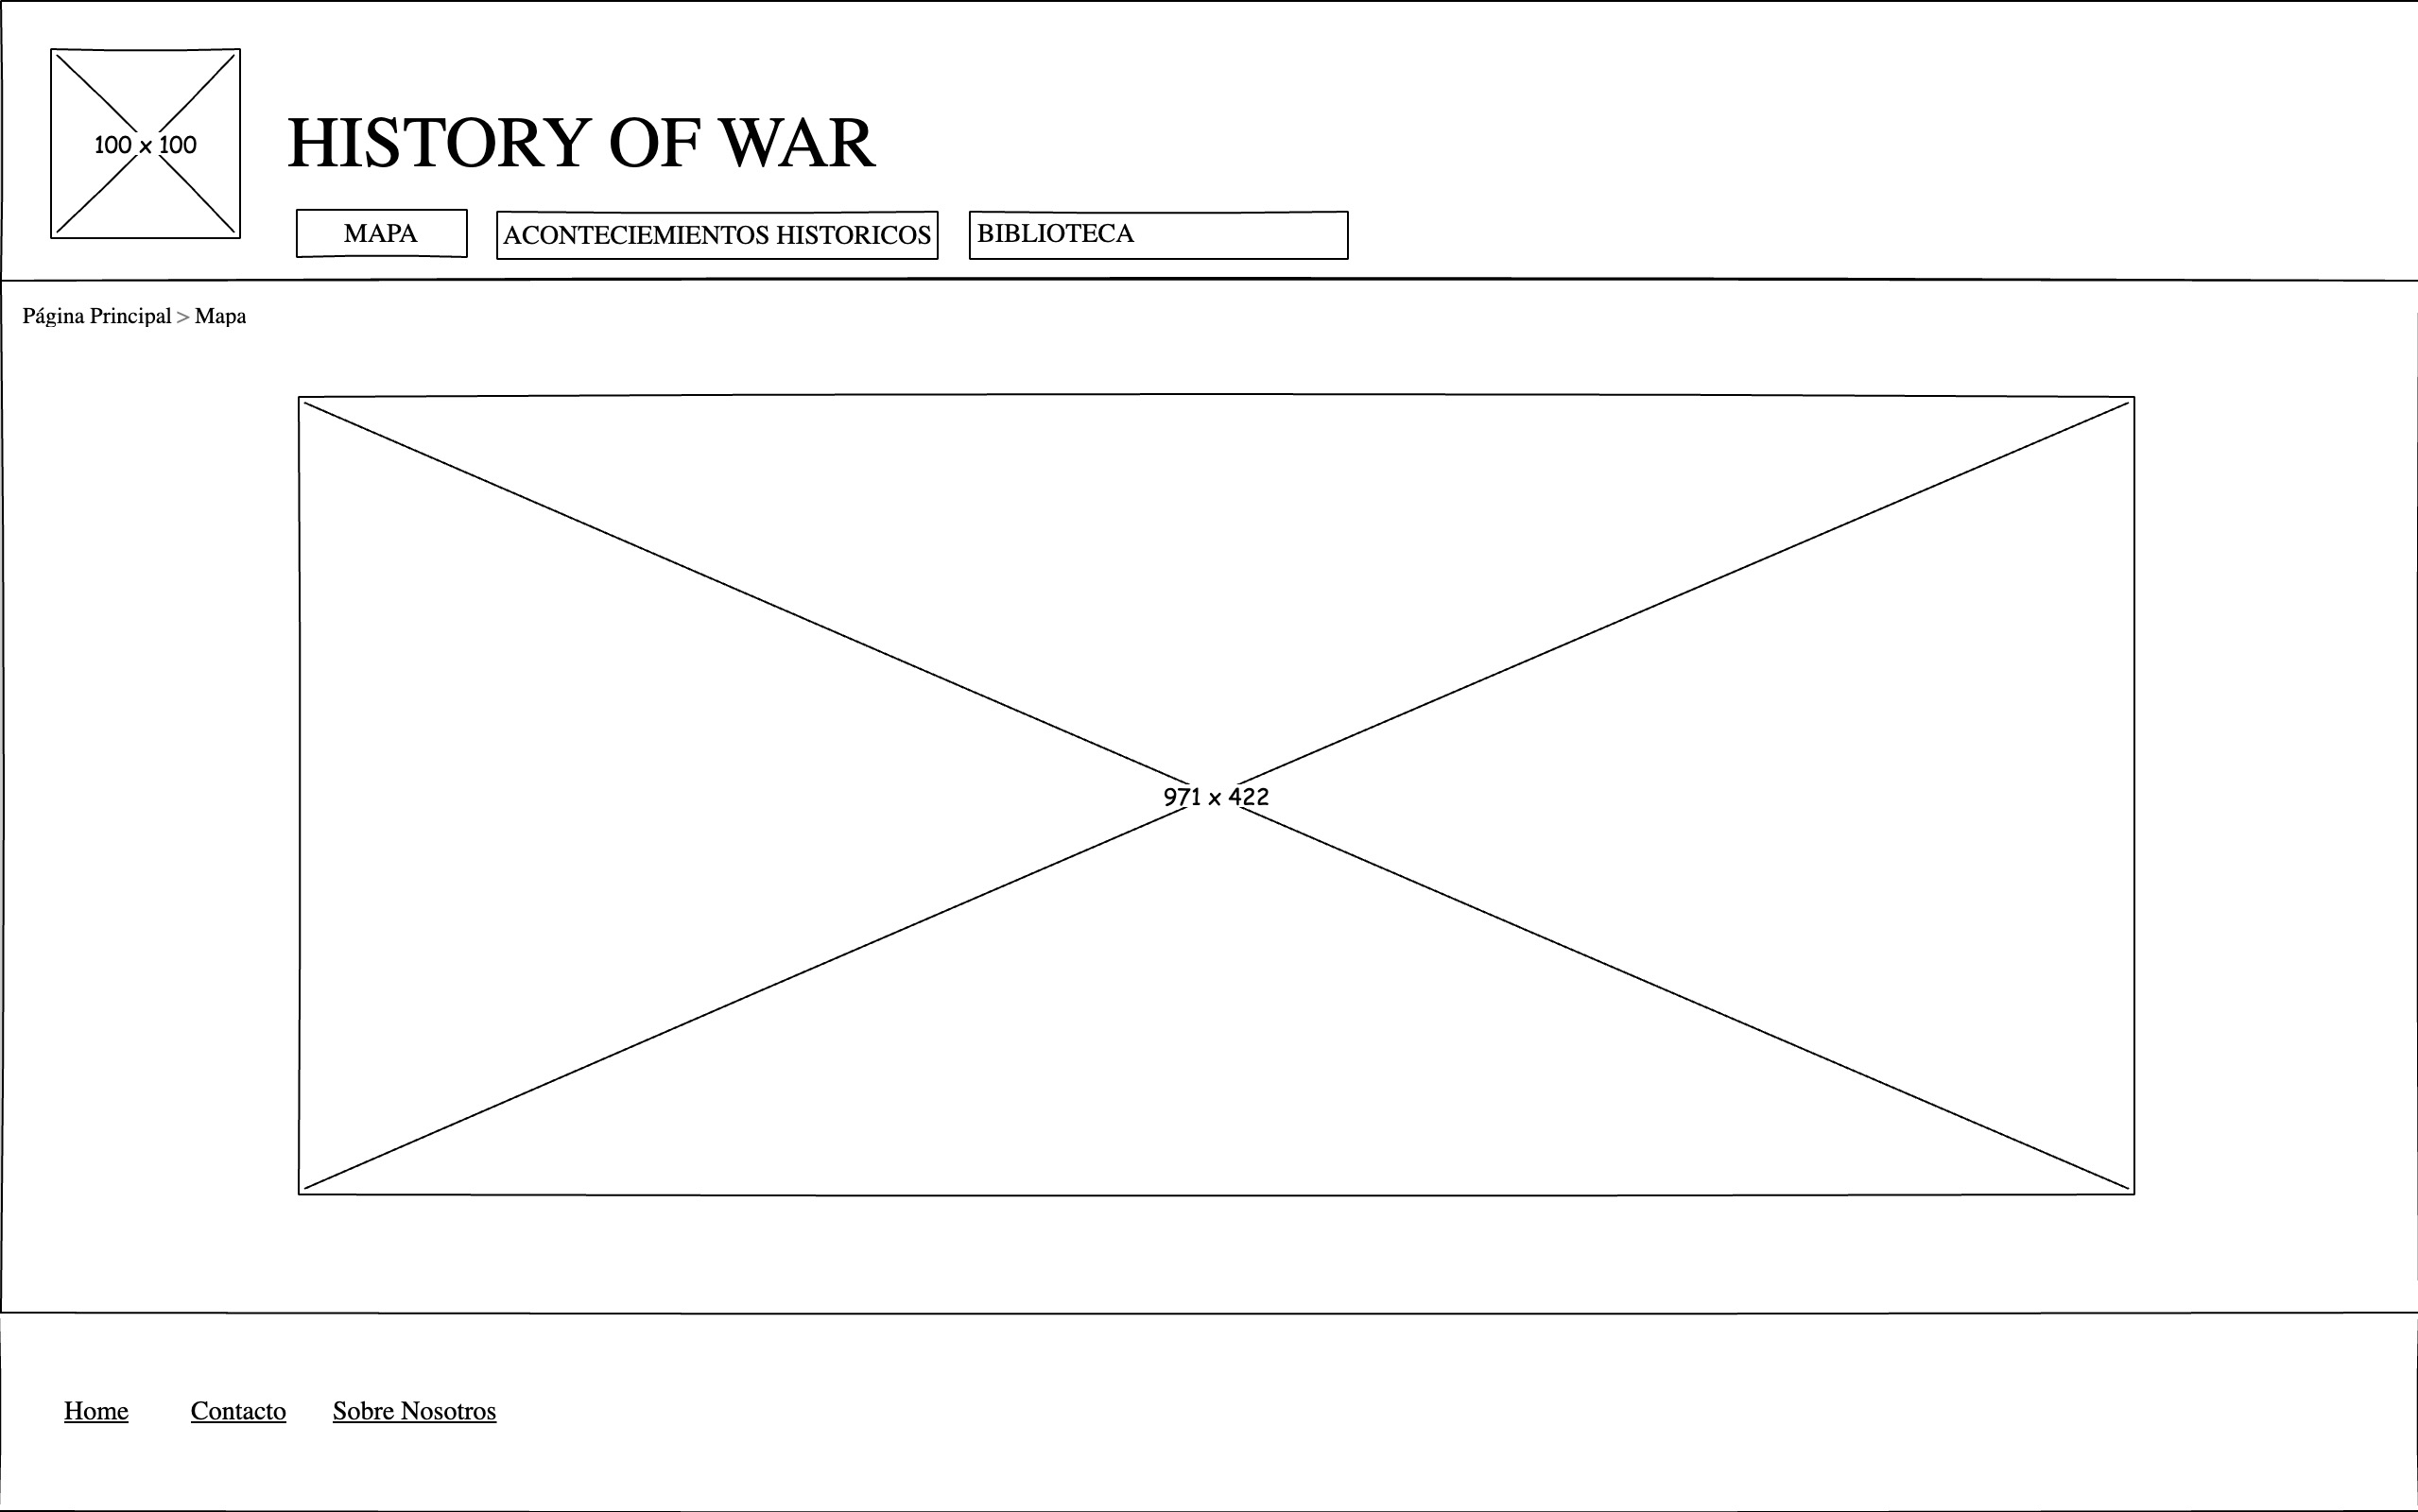
\includegraphics[width=1\textwidth]{Wireframes/Mapa.jpg}
    \caption{Mapa}
    \label{fig:mi_imagen}
\end{figure}

\begin{figure}[H]
    \centering
    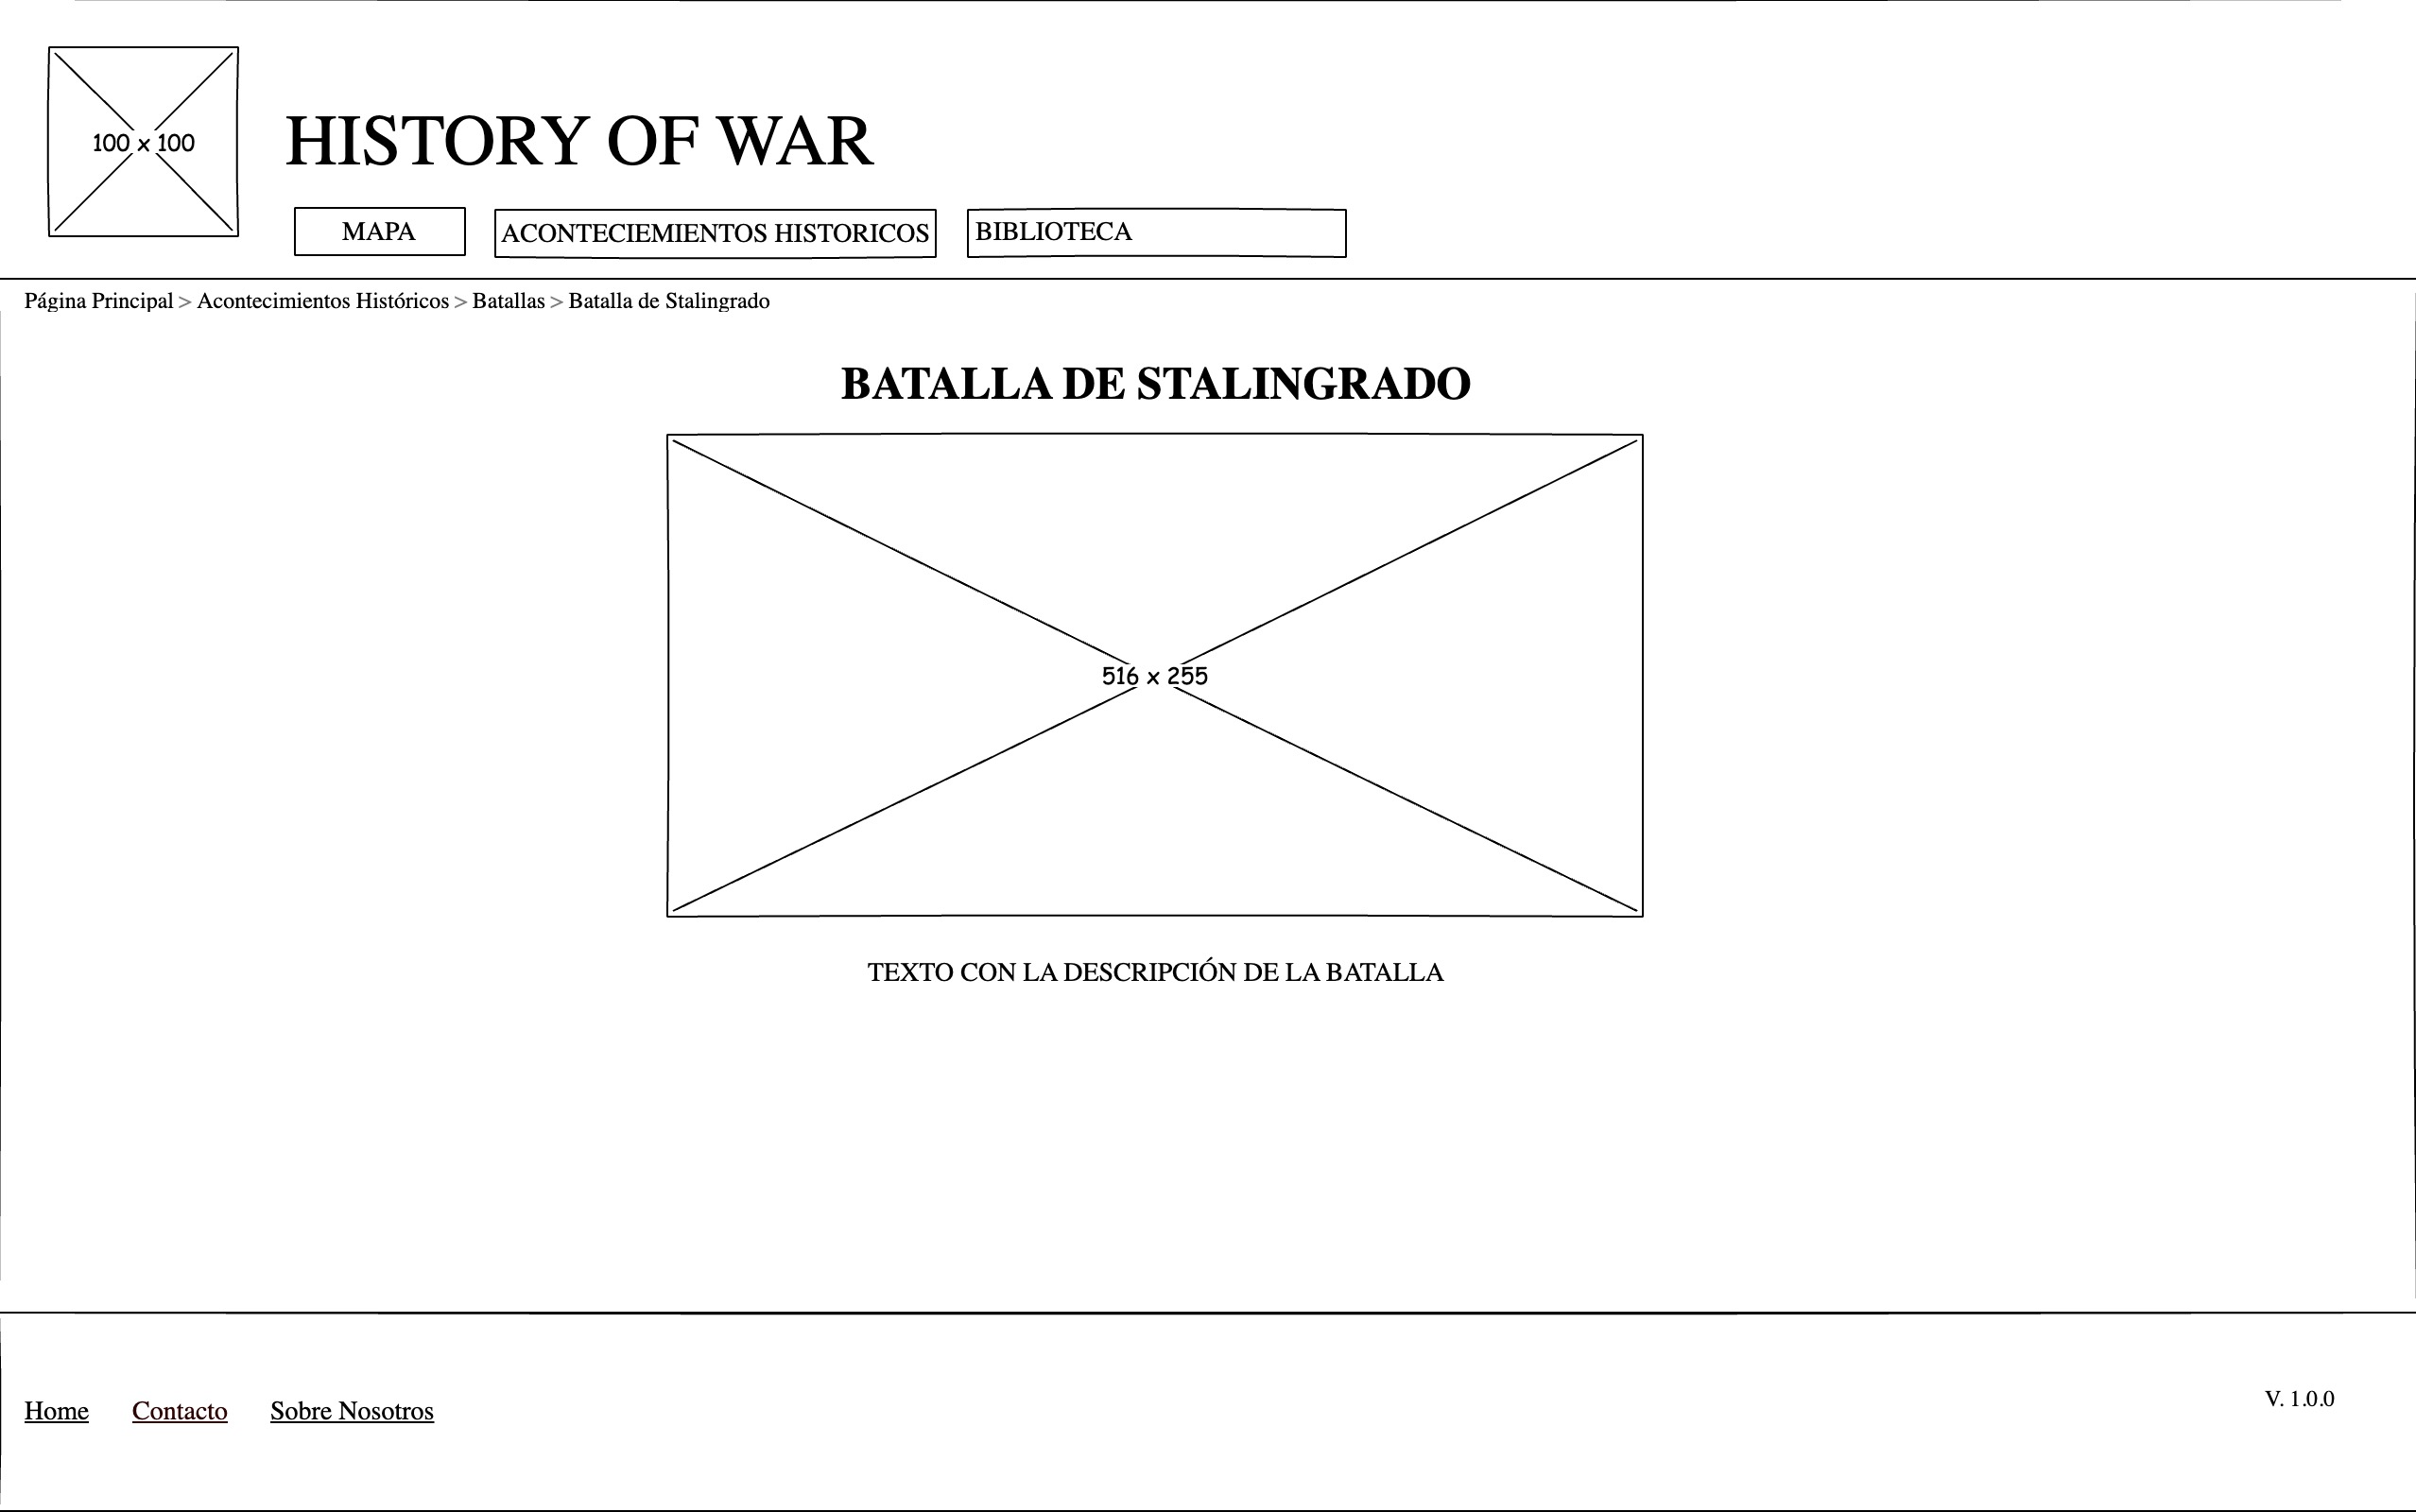
\includegraphics[width=1\textwidth]{Wireframes/EjemploBatalla.jpg}
    \caption{Ejemplo Batalla}
    \label{fig:mi_imagen}
\end{figure}

\begin{figure}[H]
    \centering
    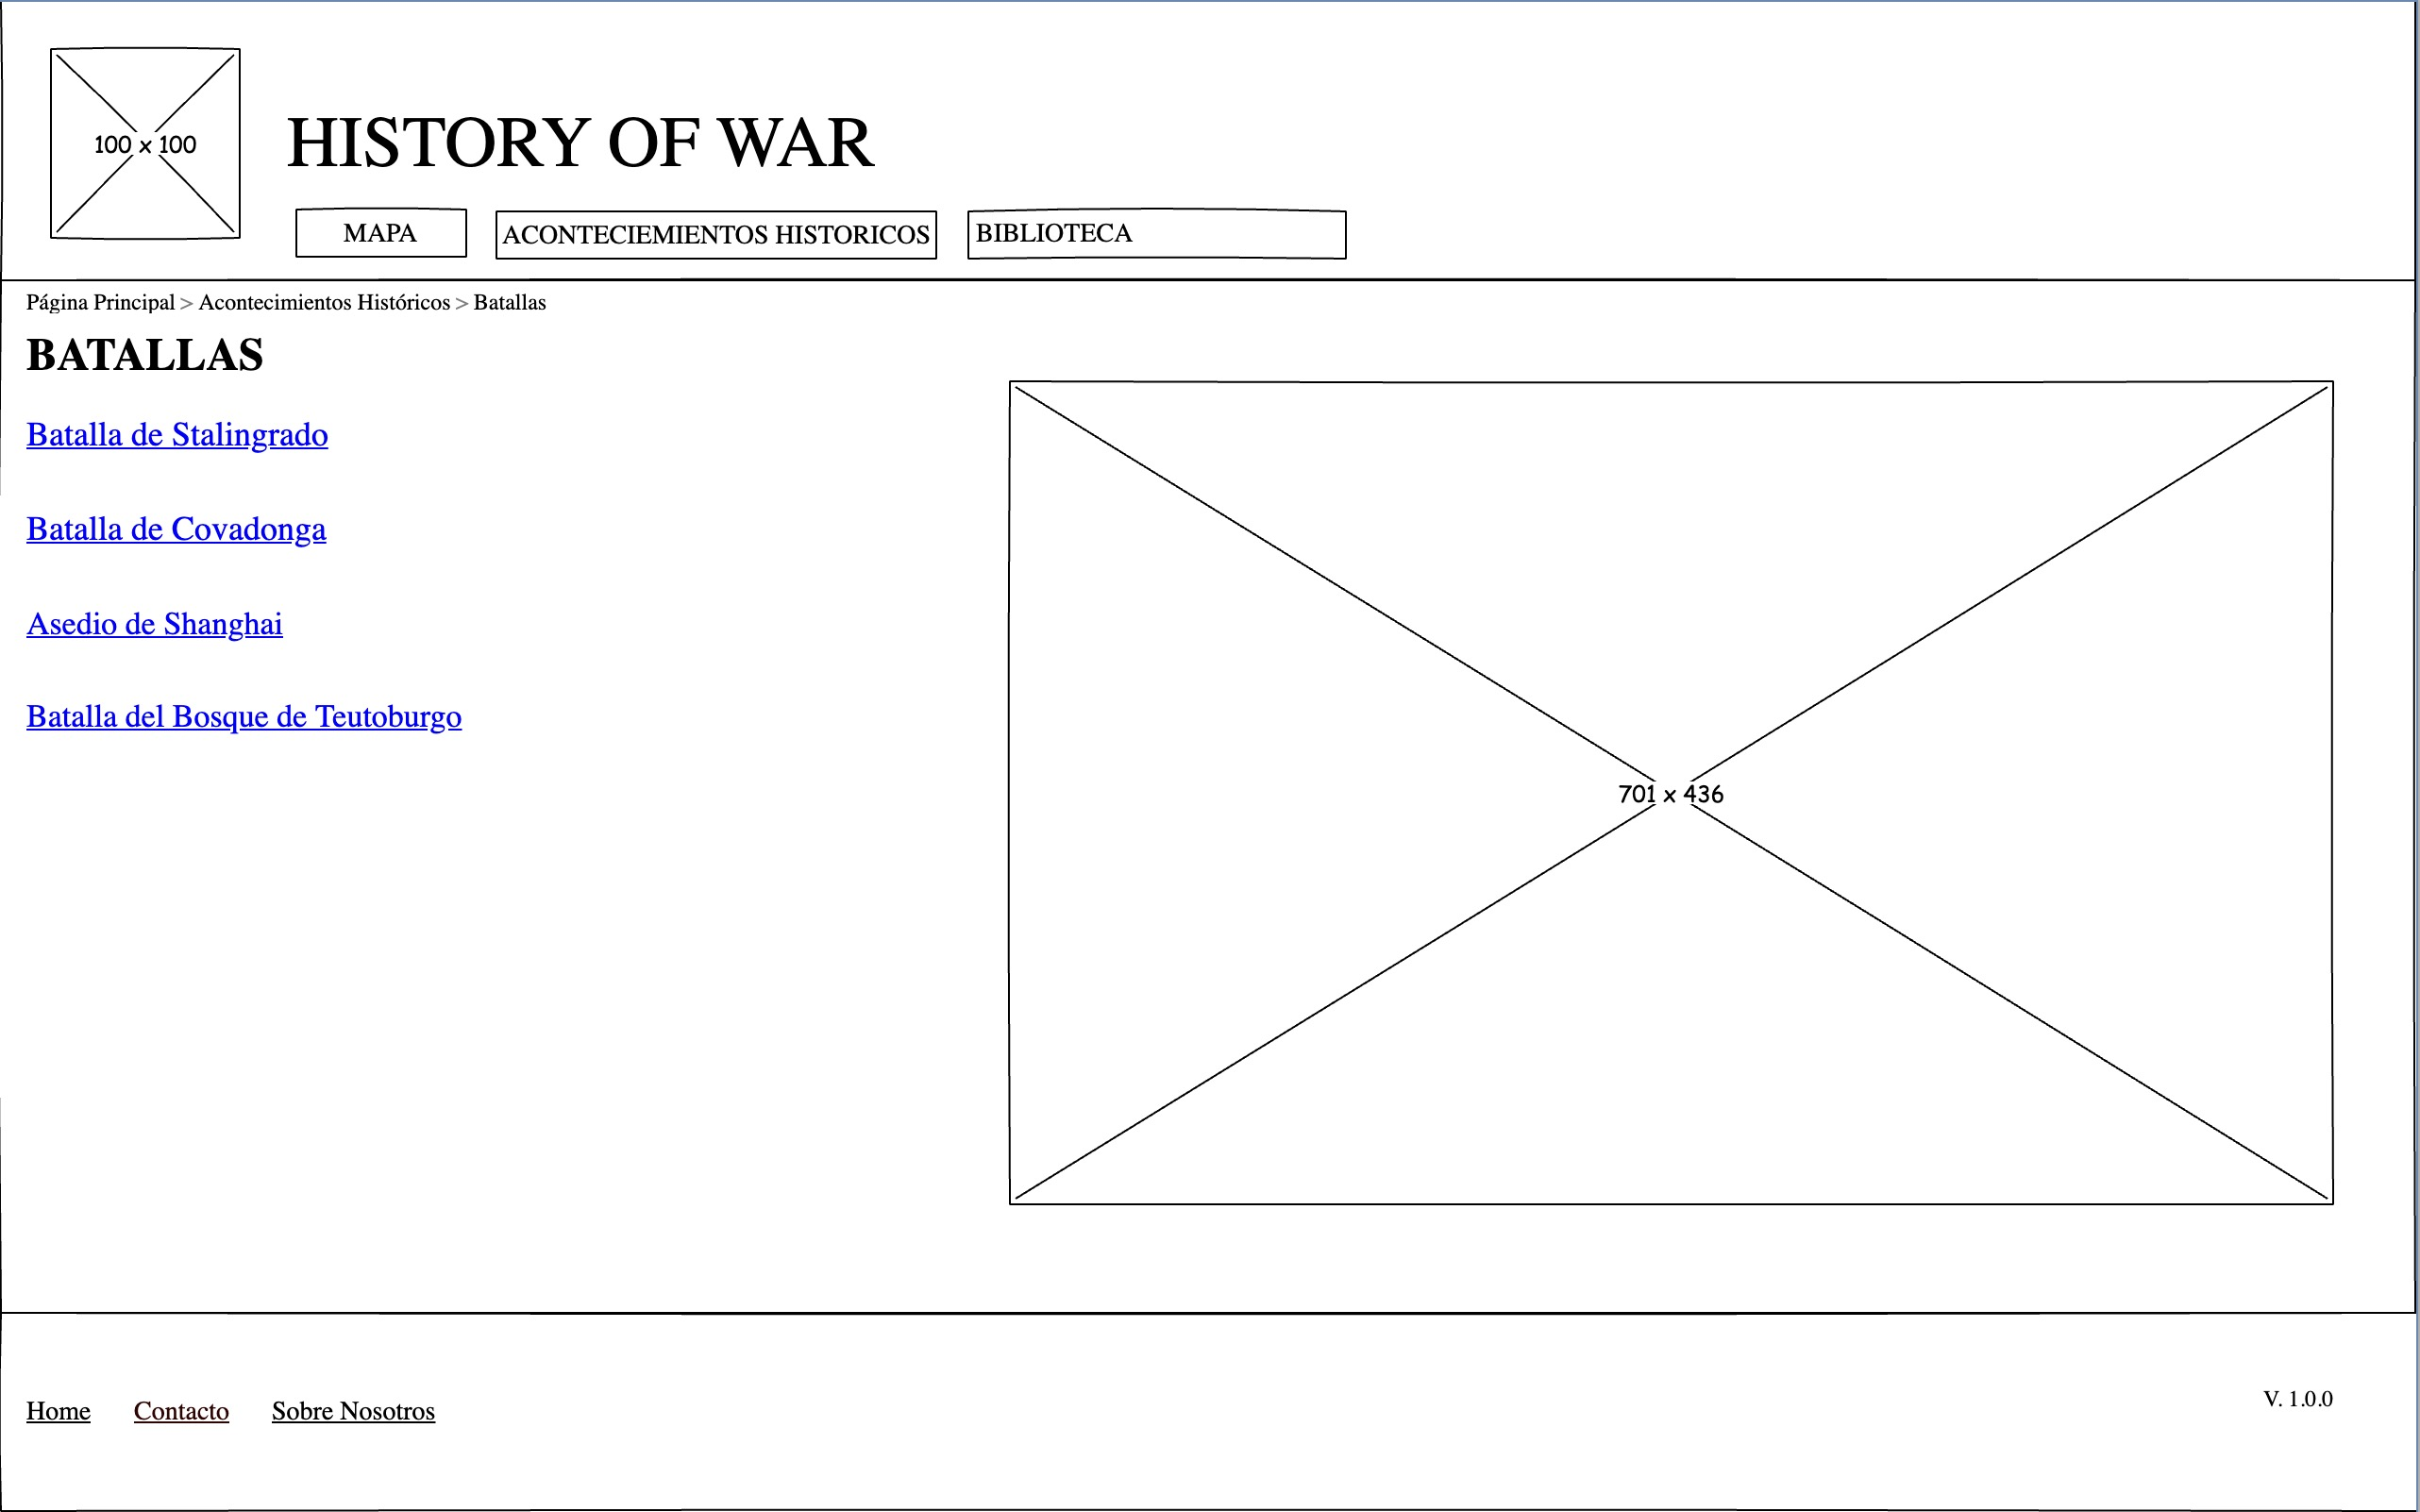
\includegraphics[width=1\textwidth]{Wireframes/Batallas.jpg}
    \caption{Batallas}
    \label{fig:mi_imagen}
\end{figure}

\begin{figure}[H]
    \centering
    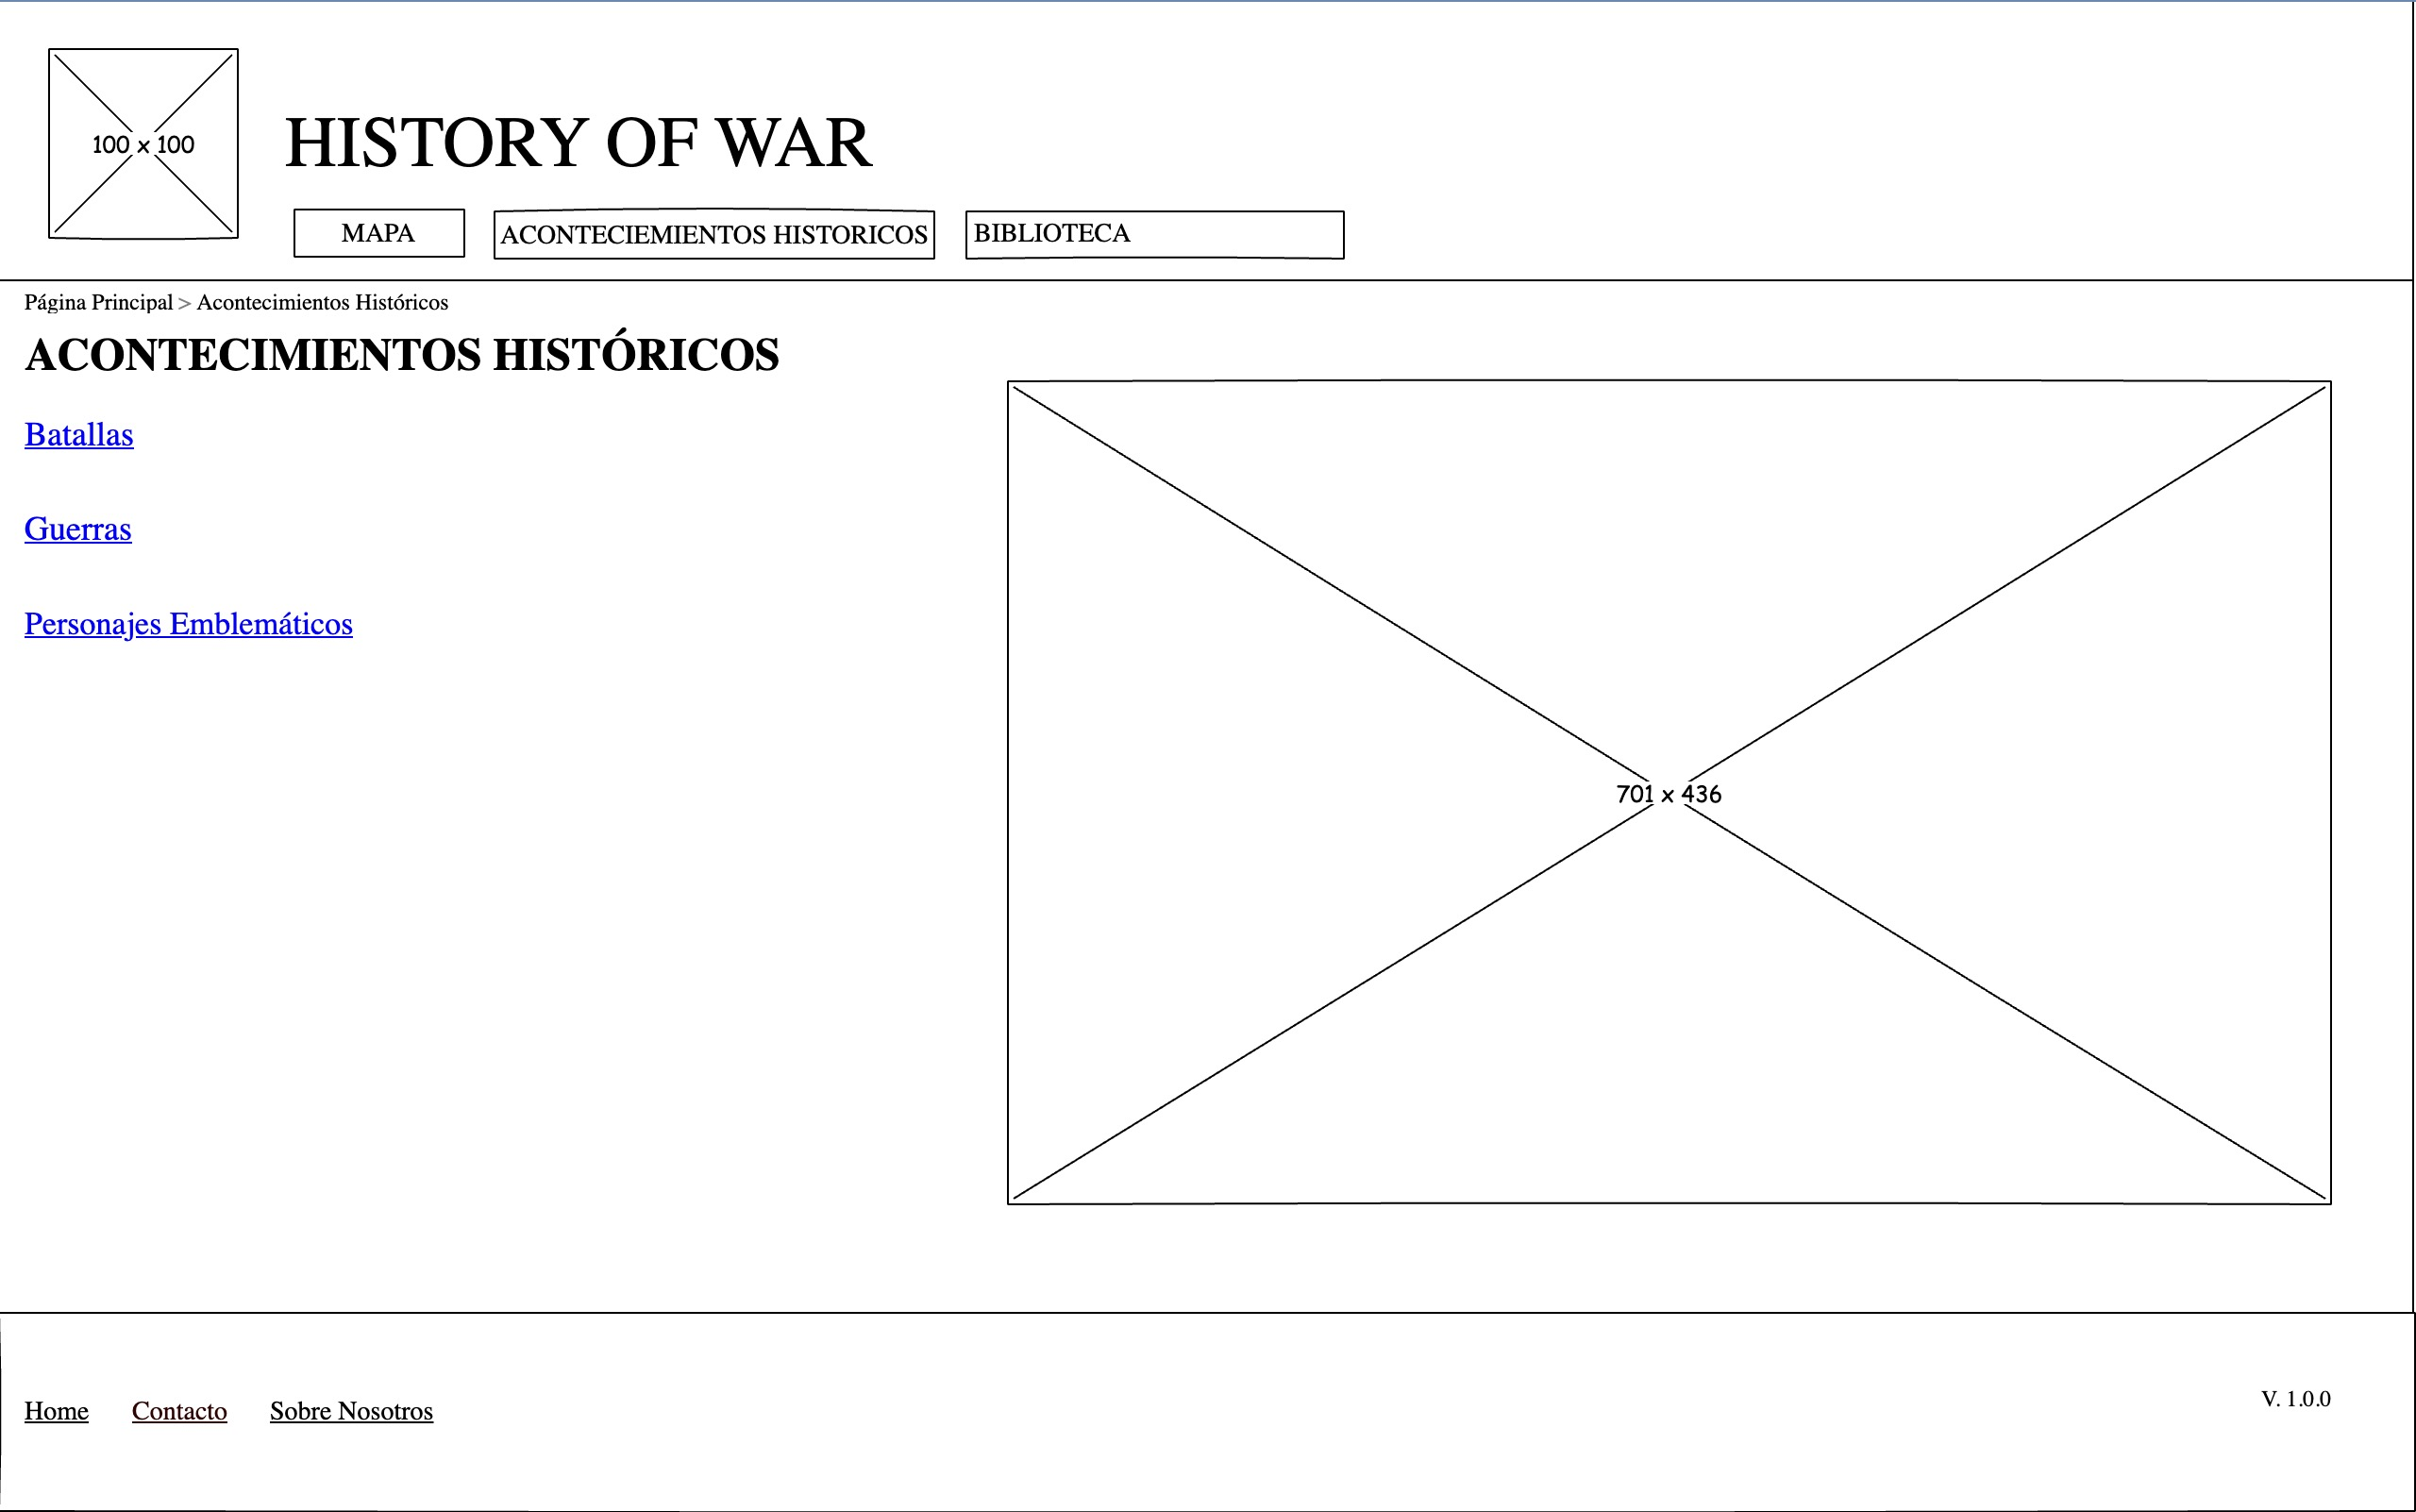
\includegraphics[width=1\textwidth]{Wireframes/AH.jpg}
    \caption{Acontecimientos Históricos}
    \label{fig:mi_imagen}
\end{figure}

\subsection{Mockups}

Los mockups son representaciones visuales de alta fidelidad que avanzan sobre la base establecida por los wireframes, ofreciendo una versión más detallada y cercana al diseño final de nuestra página web. Estas maquetas incorporan elementos de diseño gráfico, paletas de colores, tipografías y otros componentes estéticos, proporcionando una vista previa más precisa de cómo se verá y sentirá el sitio web una vez completado. Funcionan como una herramienta esencial en el proceso de diseño, facilitando la evaluación y ajuste del aspecto visual y la experiencia de usuario antes de entrar en las etapas de desarrollo técnico.

\begin{figure}[H]
    \centering
    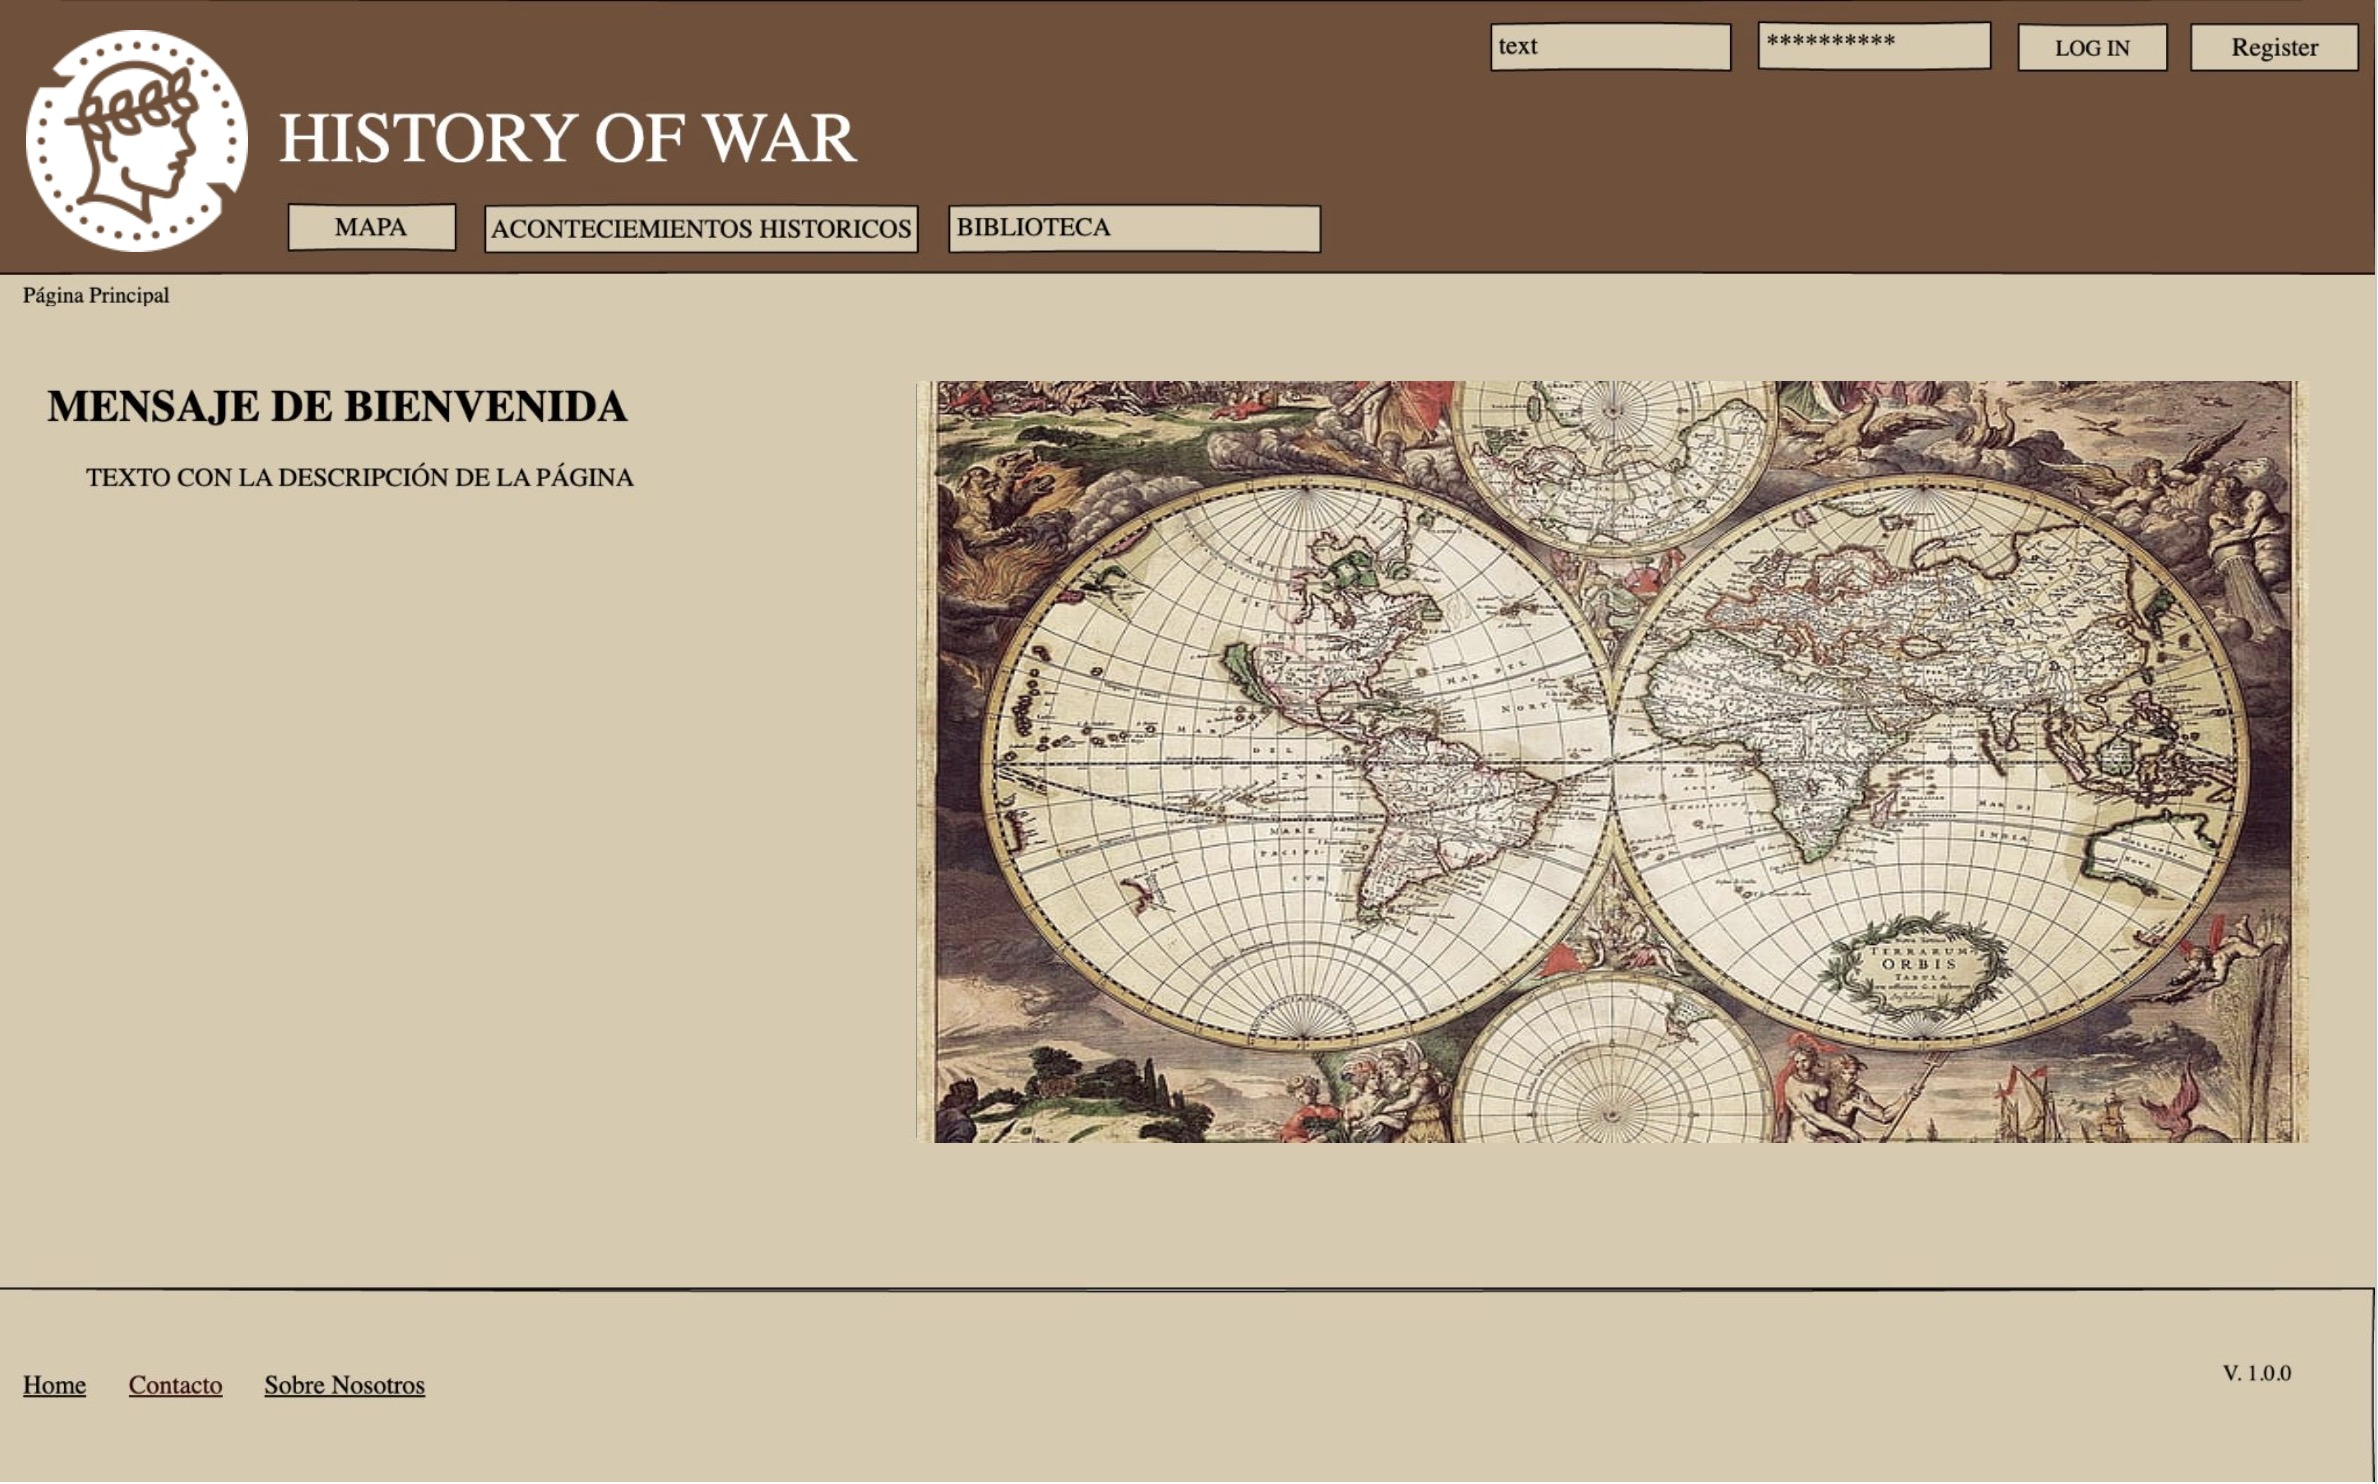
\includegraphics[width=1\textwidth]{Mockup/PaginaPrincipal (1).jpg}
    \caption{Página Principal}
    \label{fig:mi_imagen}
\end{figure}

\begin{figure}[H]
    \centering
    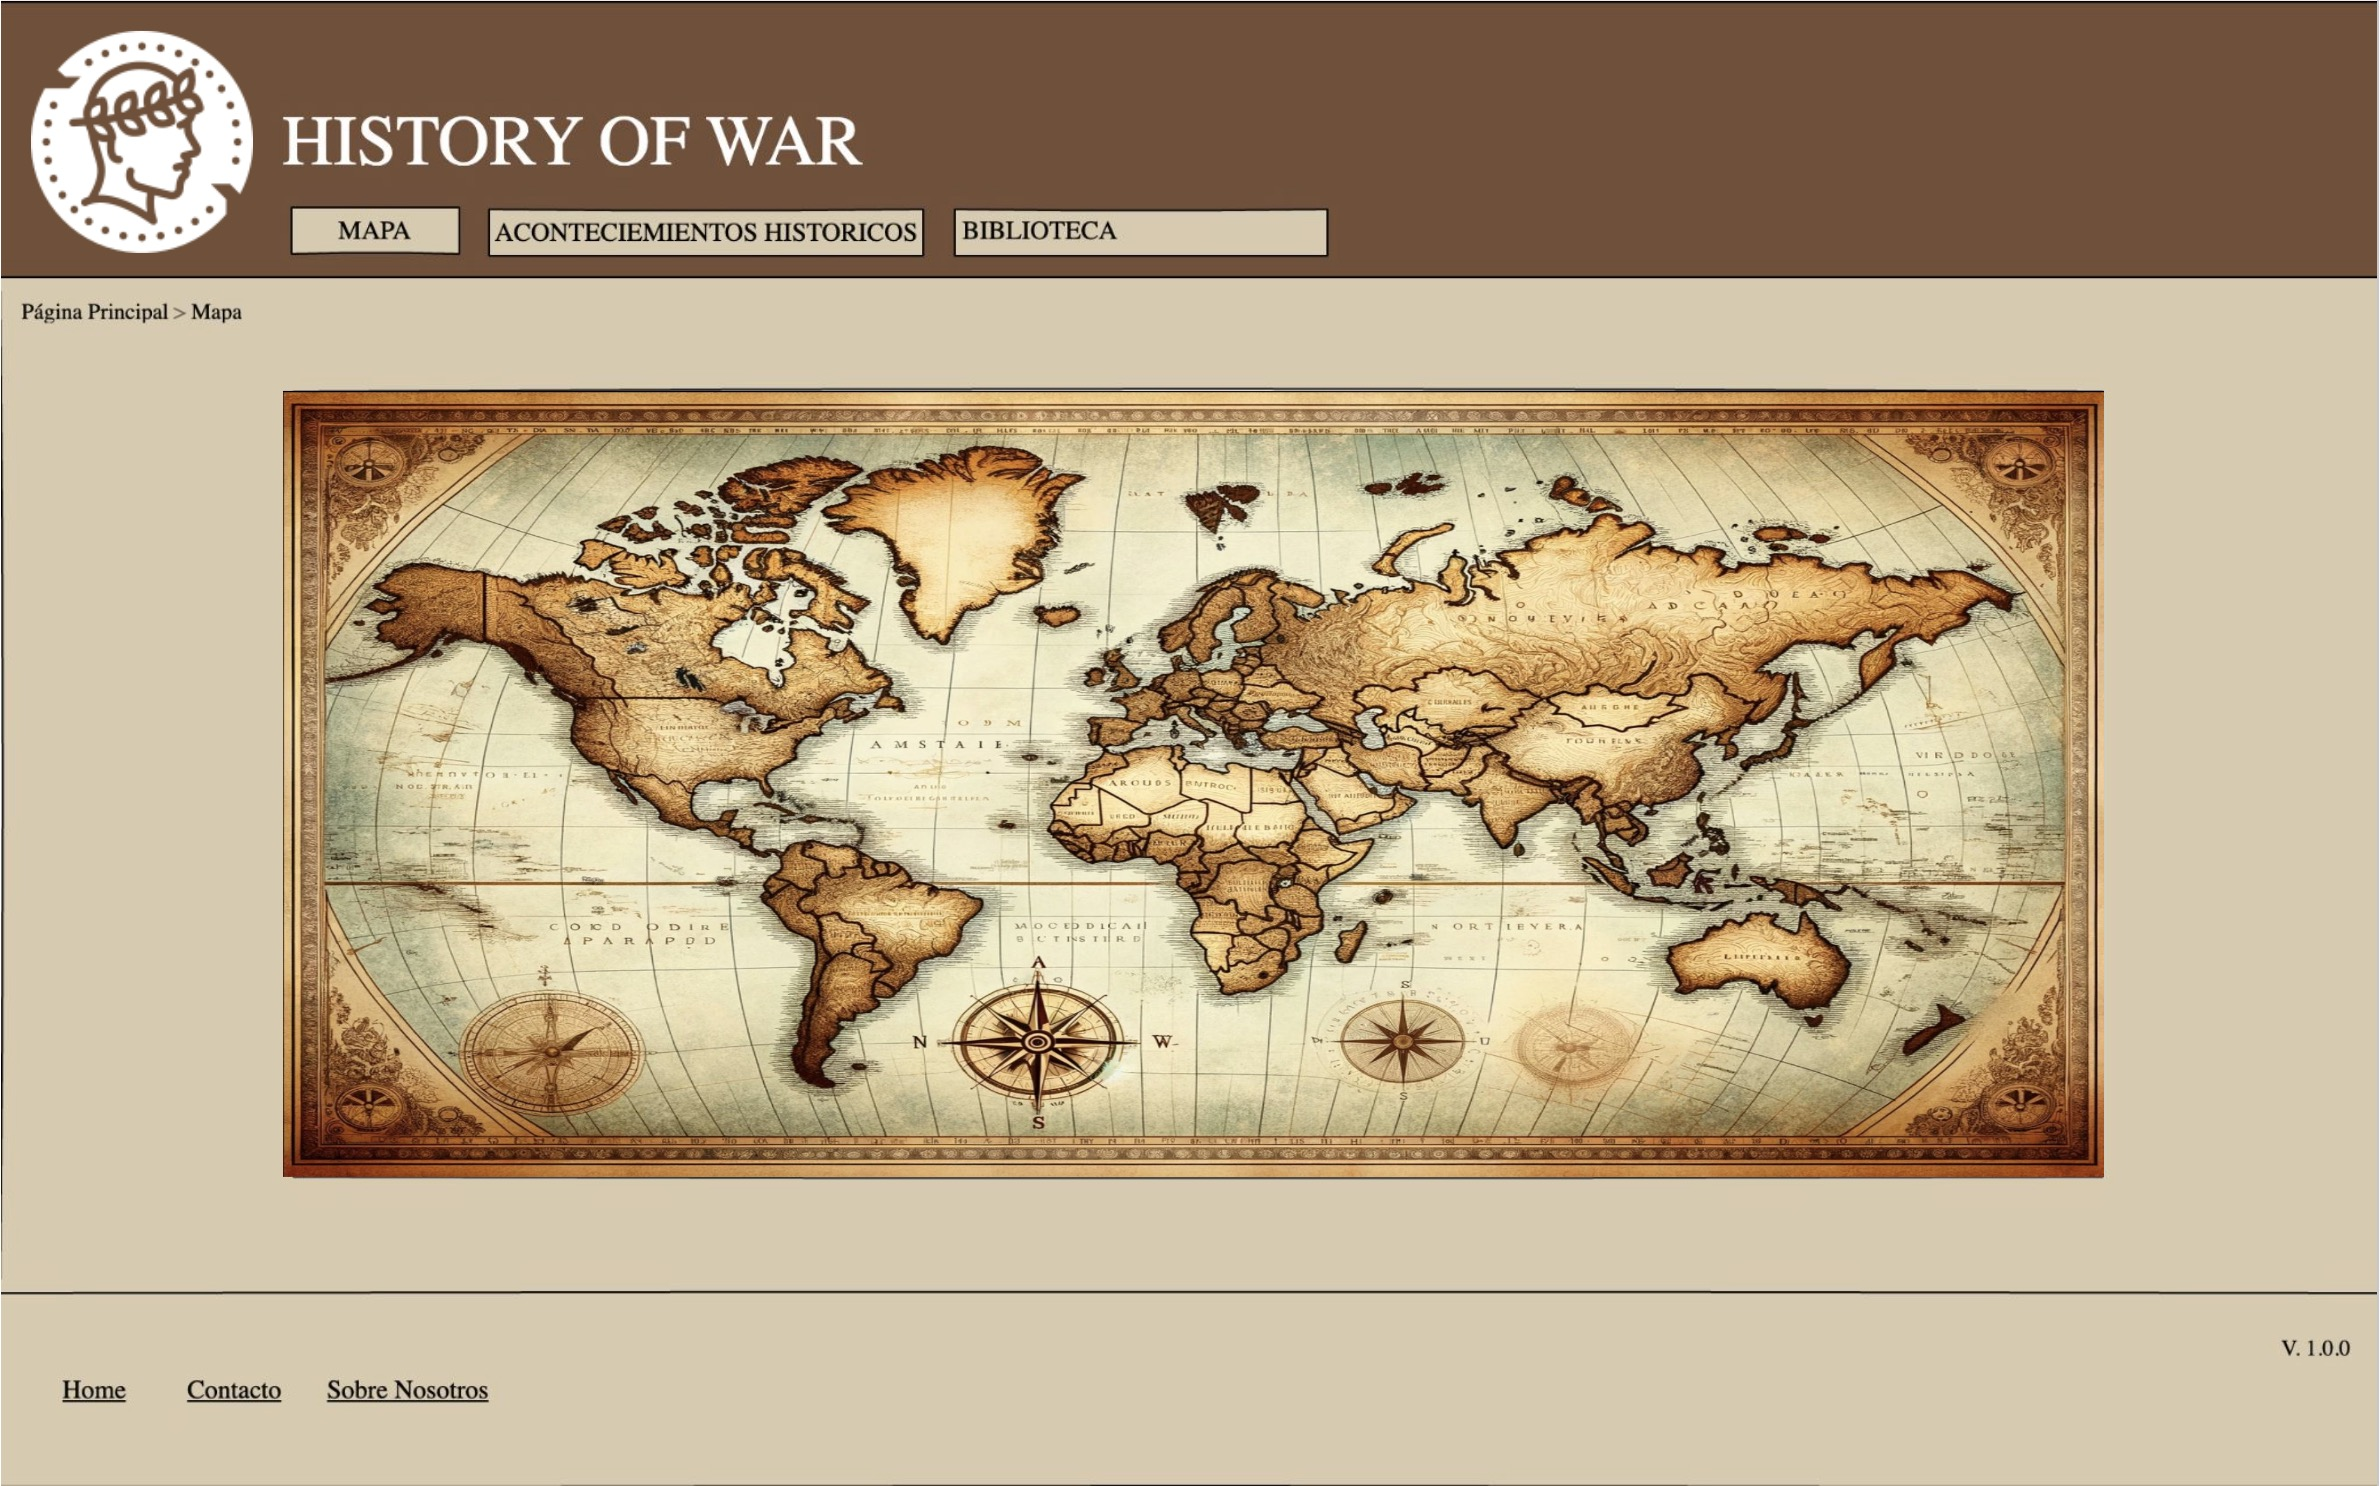
\includegraphics[width=1\textwidth]{Mockup/MapaMockup.jpg}
    \caption{Mapa}
    \label{fig:mi_imagen}
\end{figure}

\begin{figure}[H]
    \centering
    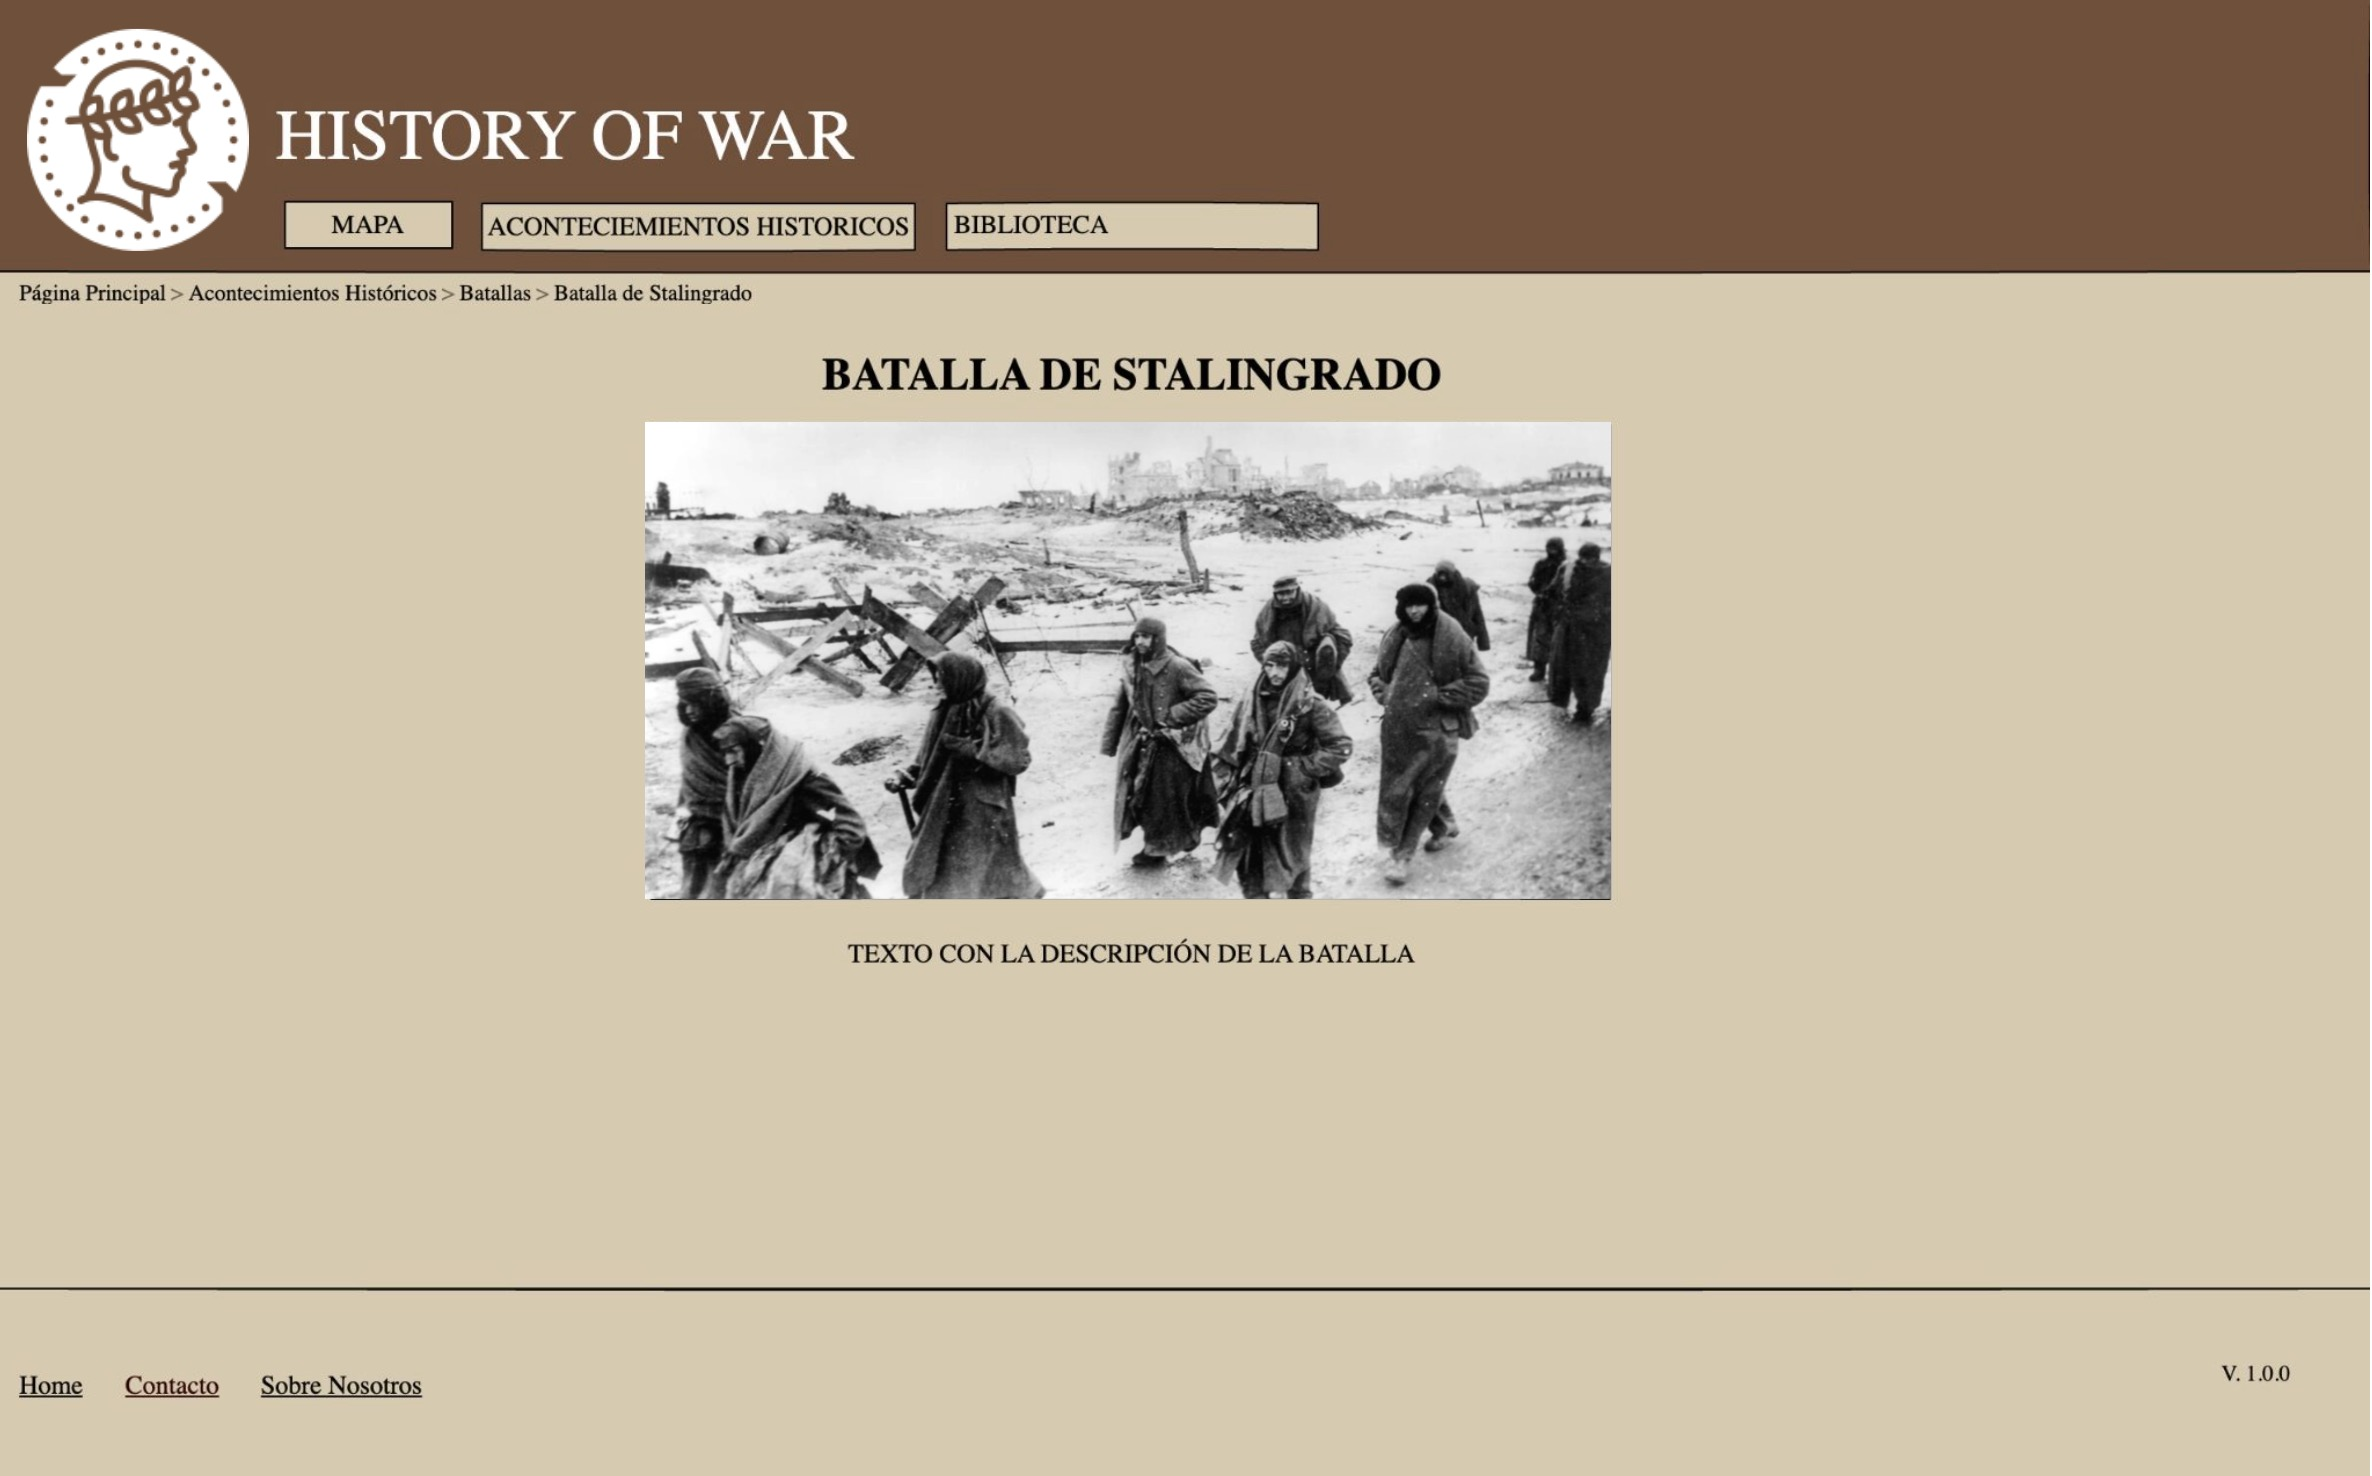
\includegraphics[width=1\textwidth]{Mockup/EjemploBatallaMockup.jpg}
    \caption{Ejemplo Batalla}
    \label{fig:mi_imagen}
\end{figure}

\begin{figure}[H]
    \centering
    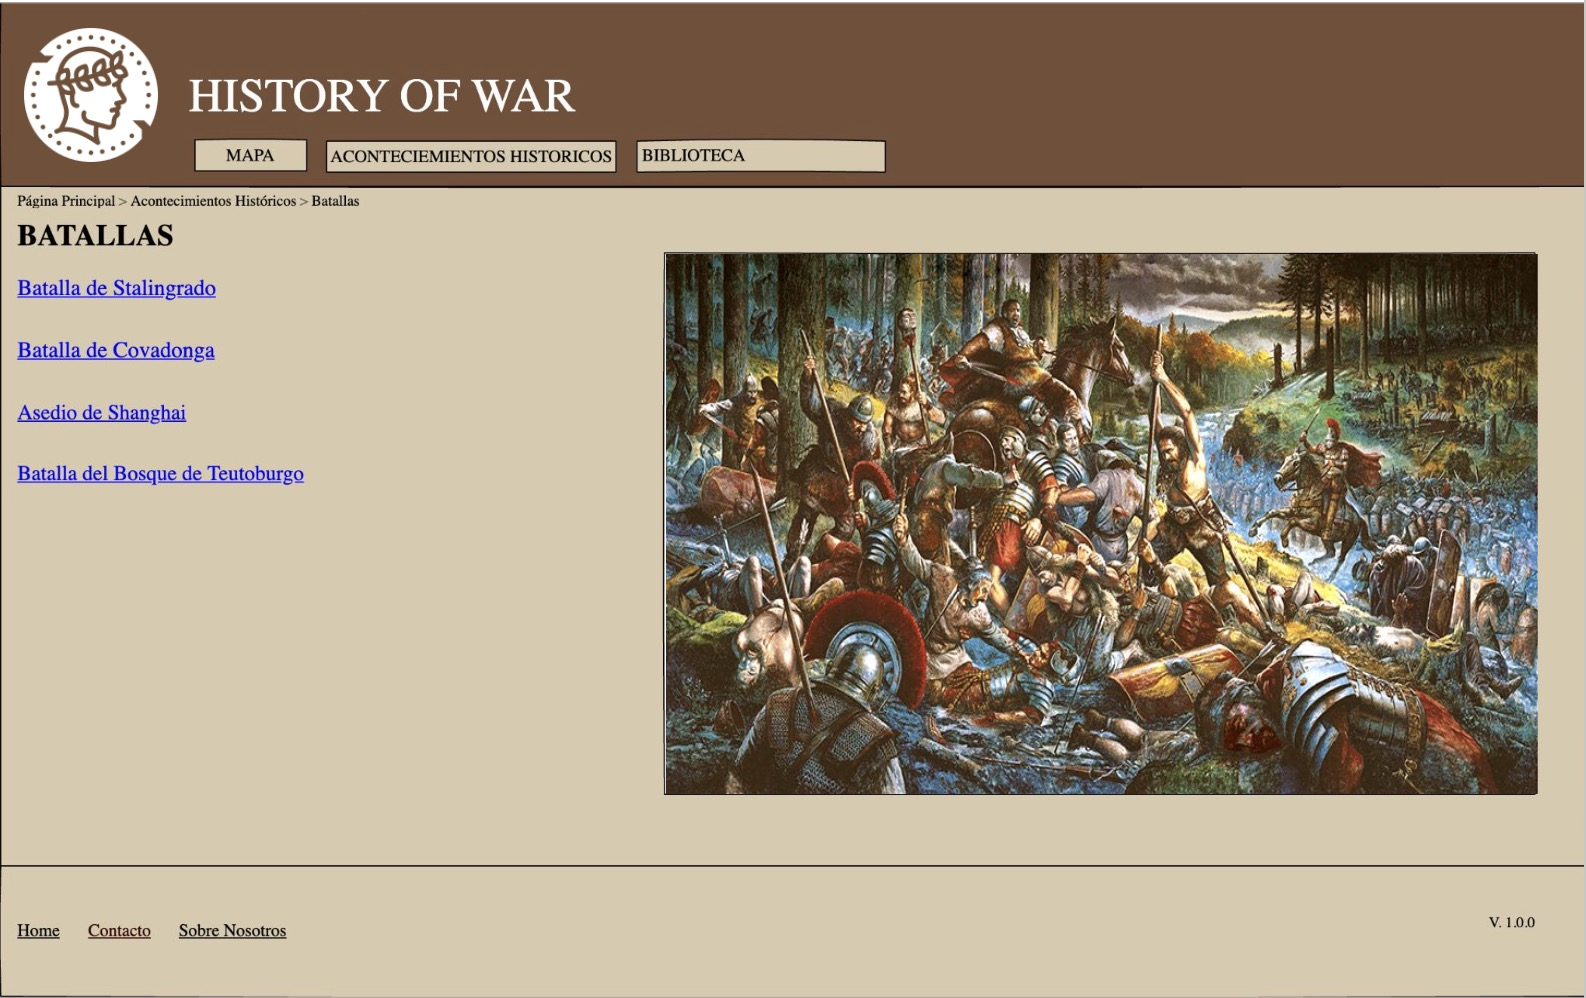
\includegraphics[width=1\textwidth]{Mockup/BatallasMockup.jpg}
    \caption{Batallas}
    \label{fig:mi_imagen}
\end{figure}

\begin{figure}[H]
    \centering
    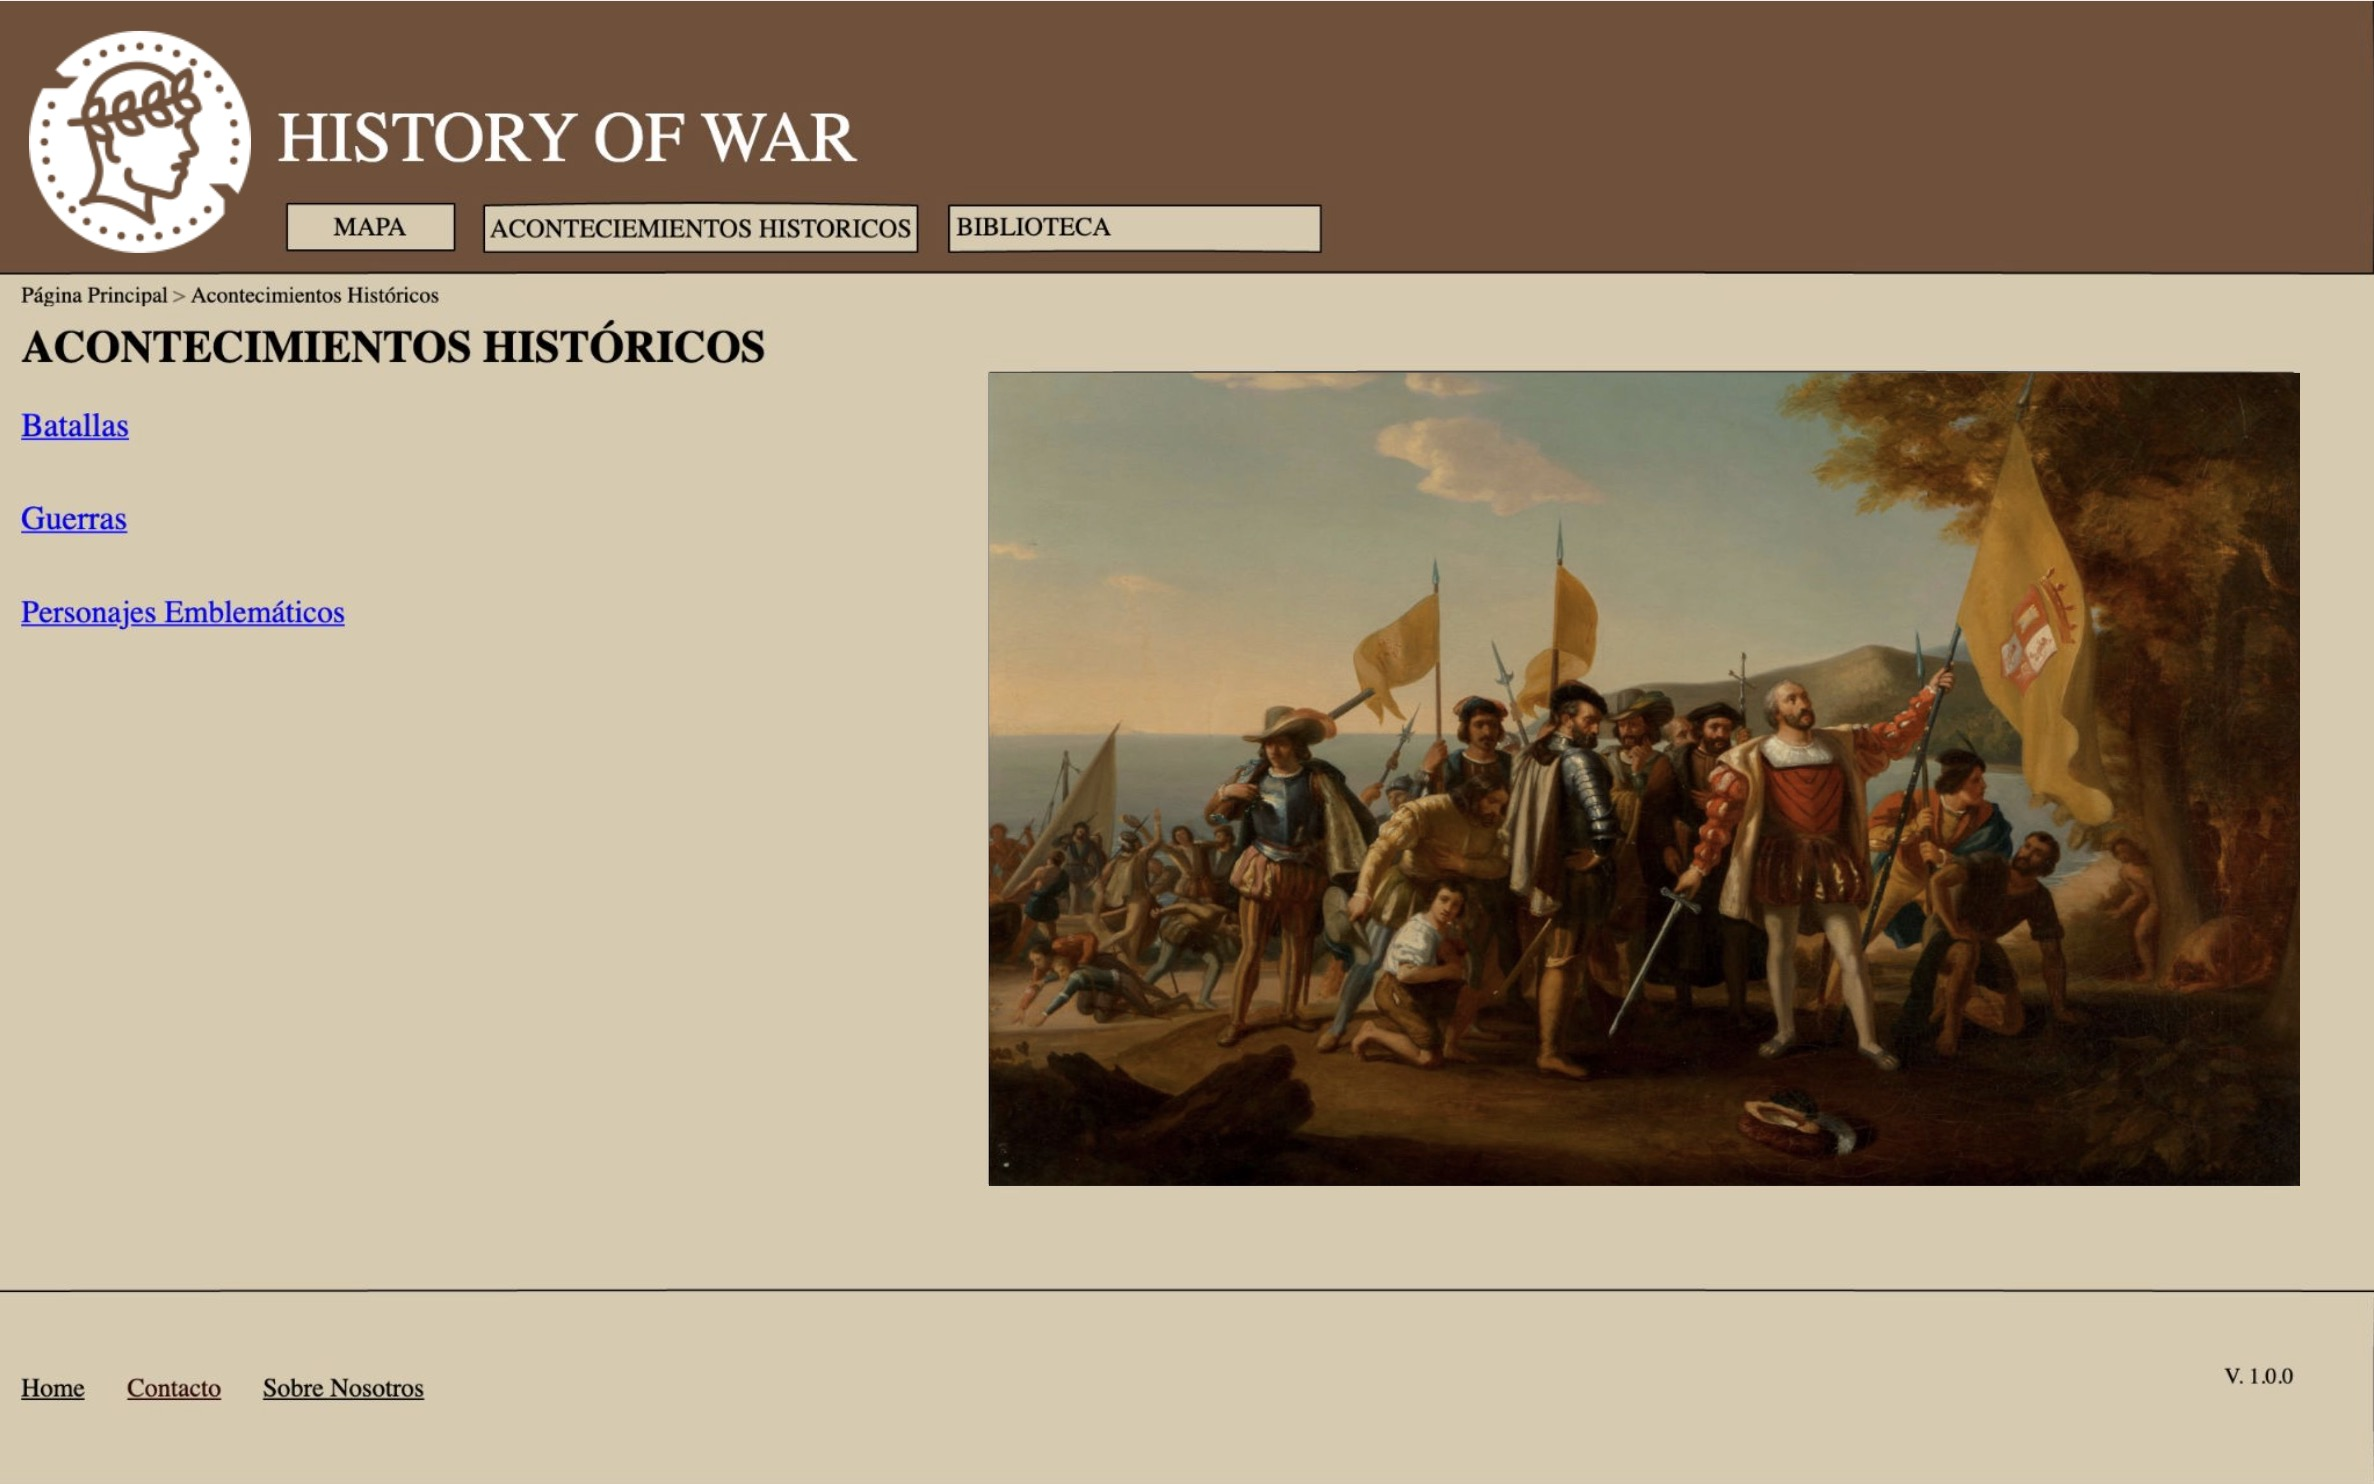
\includegraphics[width=1\textwidth]{Mockup/AHMockup.jpg}
    \caption{Acontecimientos Históricos}
    \label{fig:mi_imagen}
\end{figure}

\newpage

\section{Storyboards}

Son secuencias narrativas visuales que ilustran el flujo y la experiencia del usuario al interactuar con la página web. Estos diagramas cuentan la "historia" de cómo un usuario típico podría navegar a través del sitio, desde la página de inicio hasta la realización de acciones específicas, como realizar una compra, inscribirse en un servicio o encontrar información relevante.

\begin{figure}[H]
    \centering
    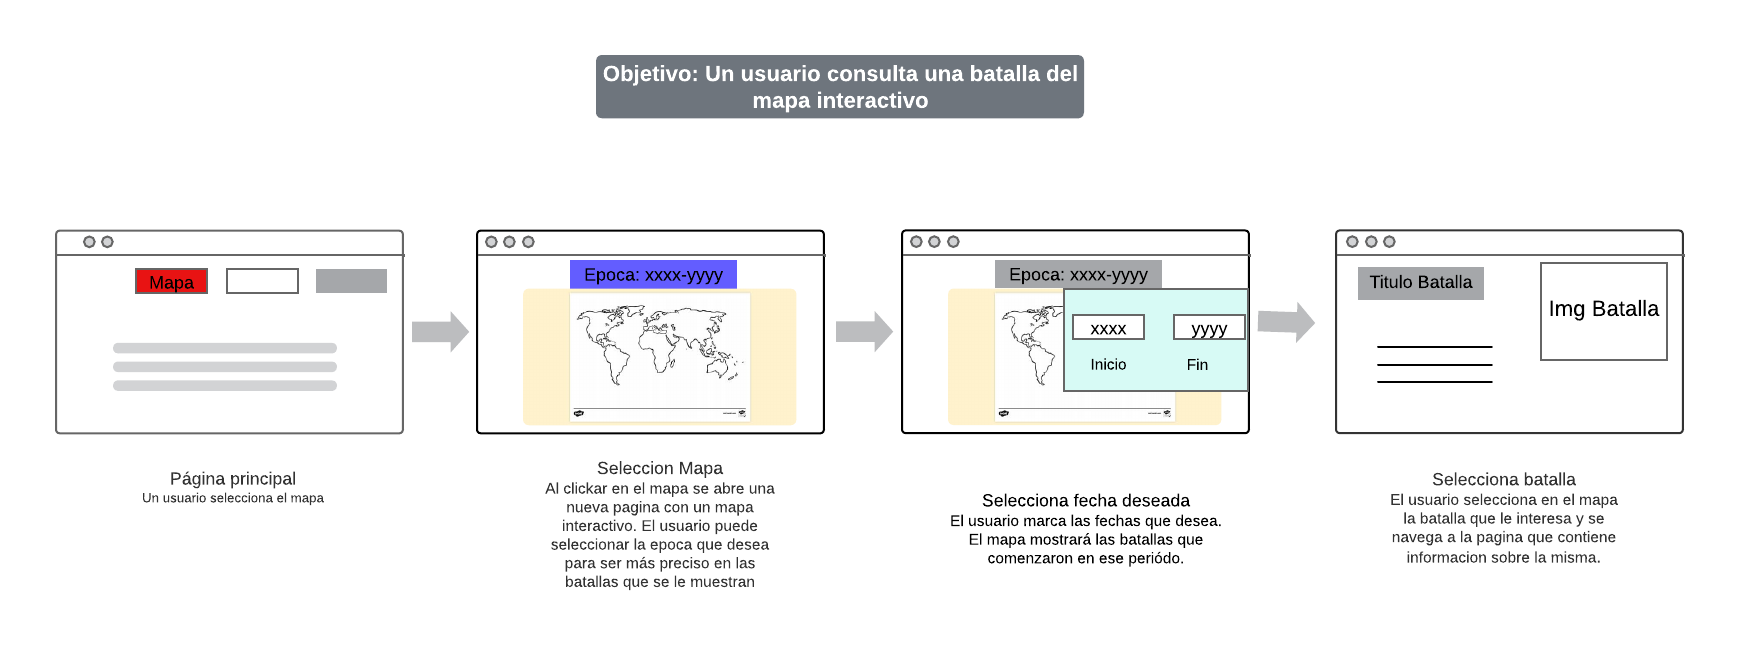
\includegraphics[width=1\textwidth]{Storyboards/StoryBoard_seleccion_batalla.png}
    \caption{Selección de Batalla}
    \label{fig:mi_imagen}
\end{figure}

\begin{figure}[H]
    \centering
    \includegraphics[width=1\textwidth]{Storyboards/StoryBoard_seleccion_libro.png}
    \caption{Selección de Libro}
    \label{fig:mi_imagen}
\end{figure}

\begin{figure}[H]
    \centering
    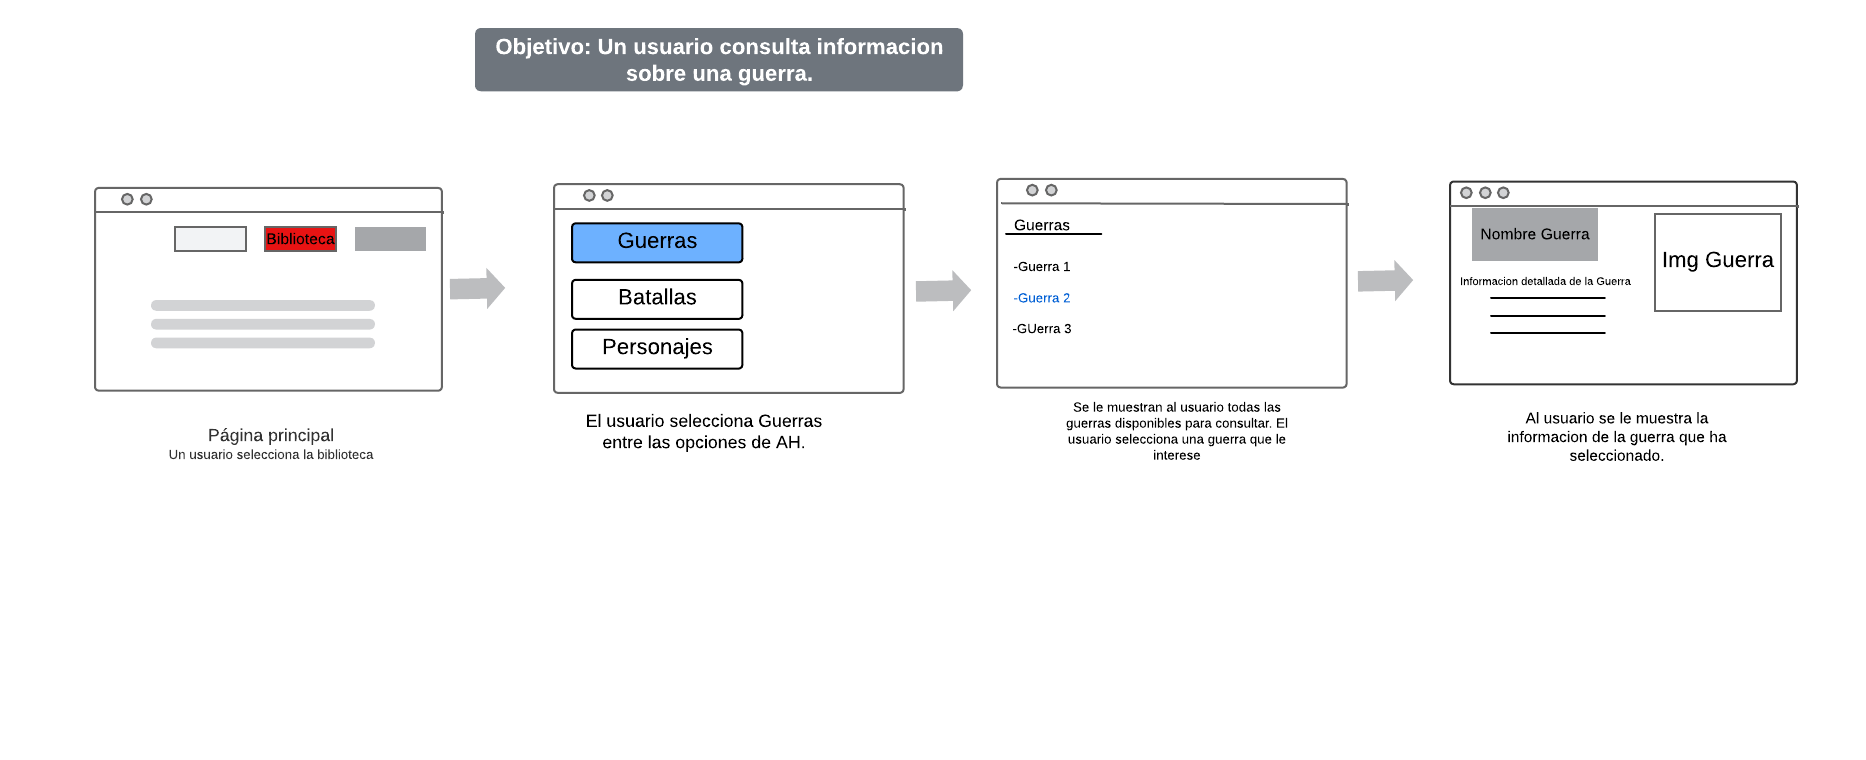
\includegraphics[width=1\textwidth]{Storyboards/StoryBoard_seleccion_guerra.png}
    \caption{Selección de Guerra}
    \label{fig:mi_imagen}
\end{figure}

\begin{figure}[H]
    \centering
    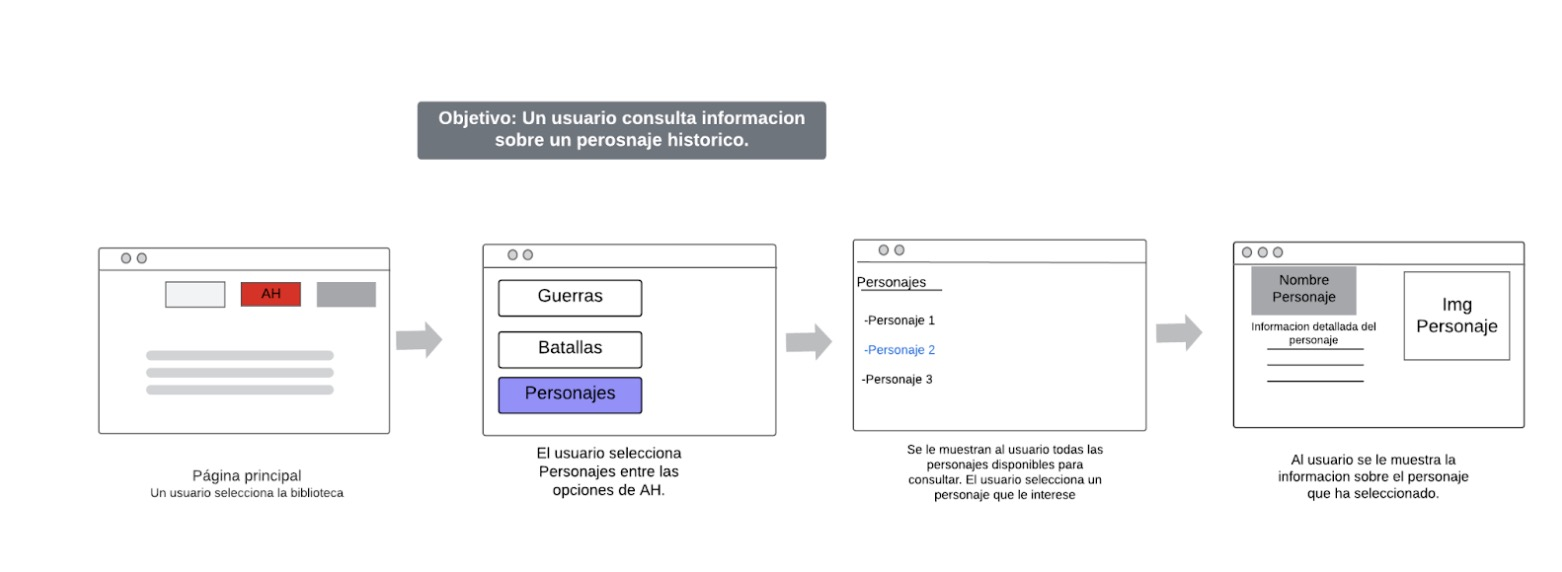
\includegraphics[width=1\textwidth]{Storyboards/StoryboardPersonaje.jpg}
    \caption{Selección de Personaje}
    \label{fig:mi_imagen}
\end{figure}

\begin{figure}[H]
    \centering
    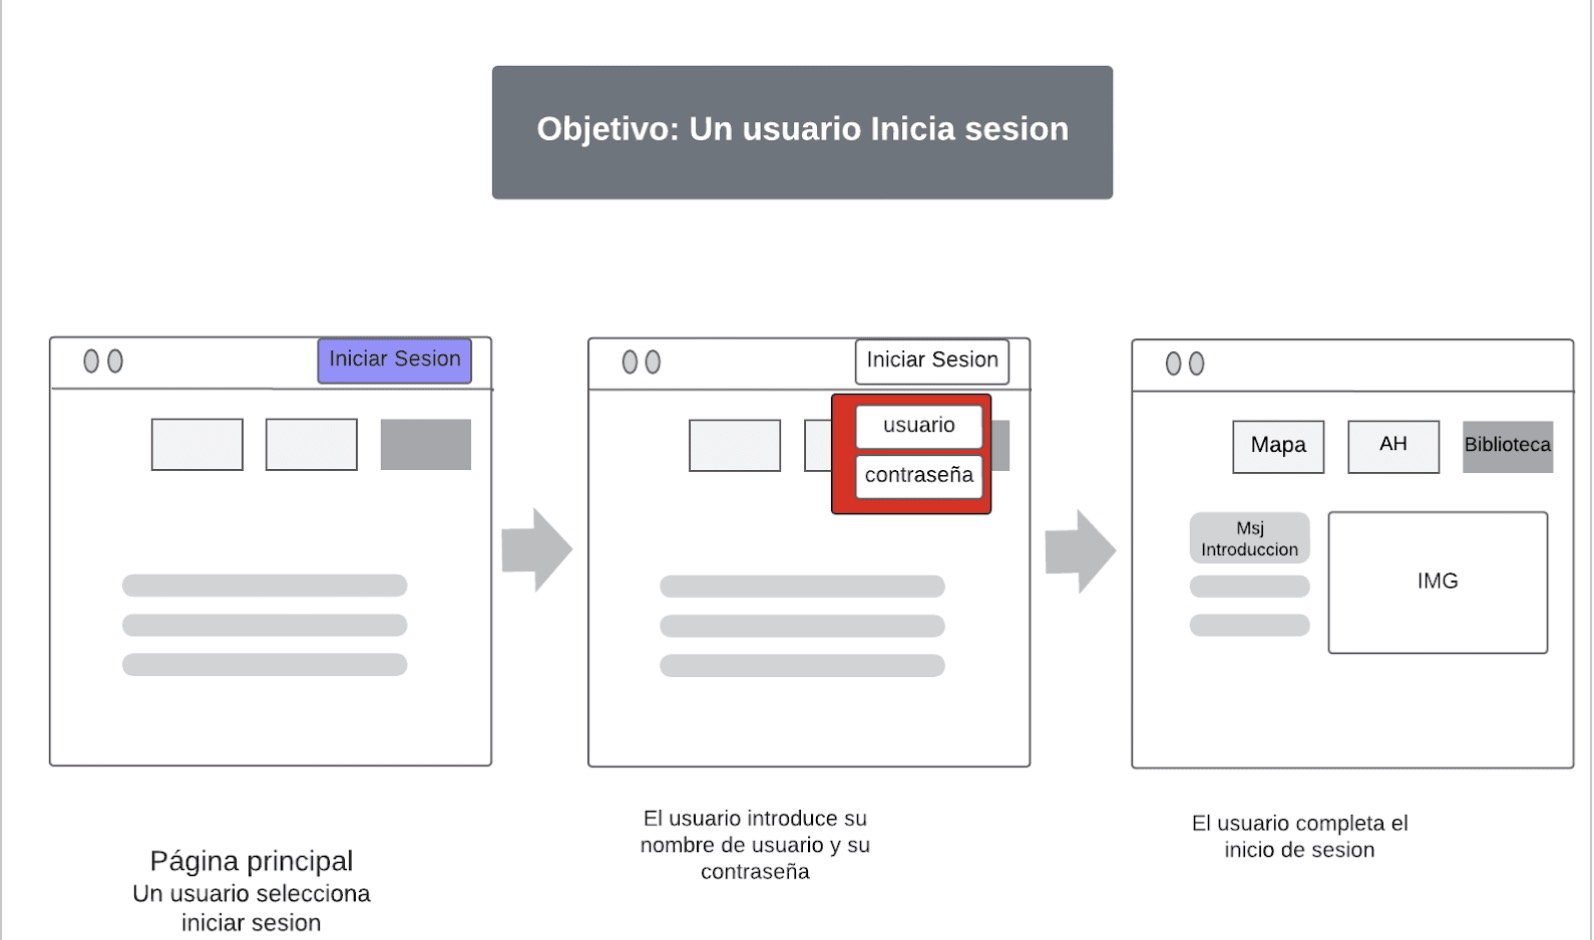
\includegraphics[width=1\textwidth]{Storyboards/StroryBoardInicioSesion.jpg}
    \caption{Inicio de Sesión}
    \label{fig:mi_imagen}
\end{figure}

\newpage

\section{Estructura de Ficheros y Carpetas}

La estructura de ficheros y carpetas en un proyecto web es esencial para mantener el orden y facilitar el desarrollo y mantenimiento del sitio. Esta organización comprende la disposición sistemática de archivos HTML, hojas de estilo CSS, scripts de JavaScript, imágenes, fuentes y otros recursos digitales.

\begin{figure}[H]
    \centering
    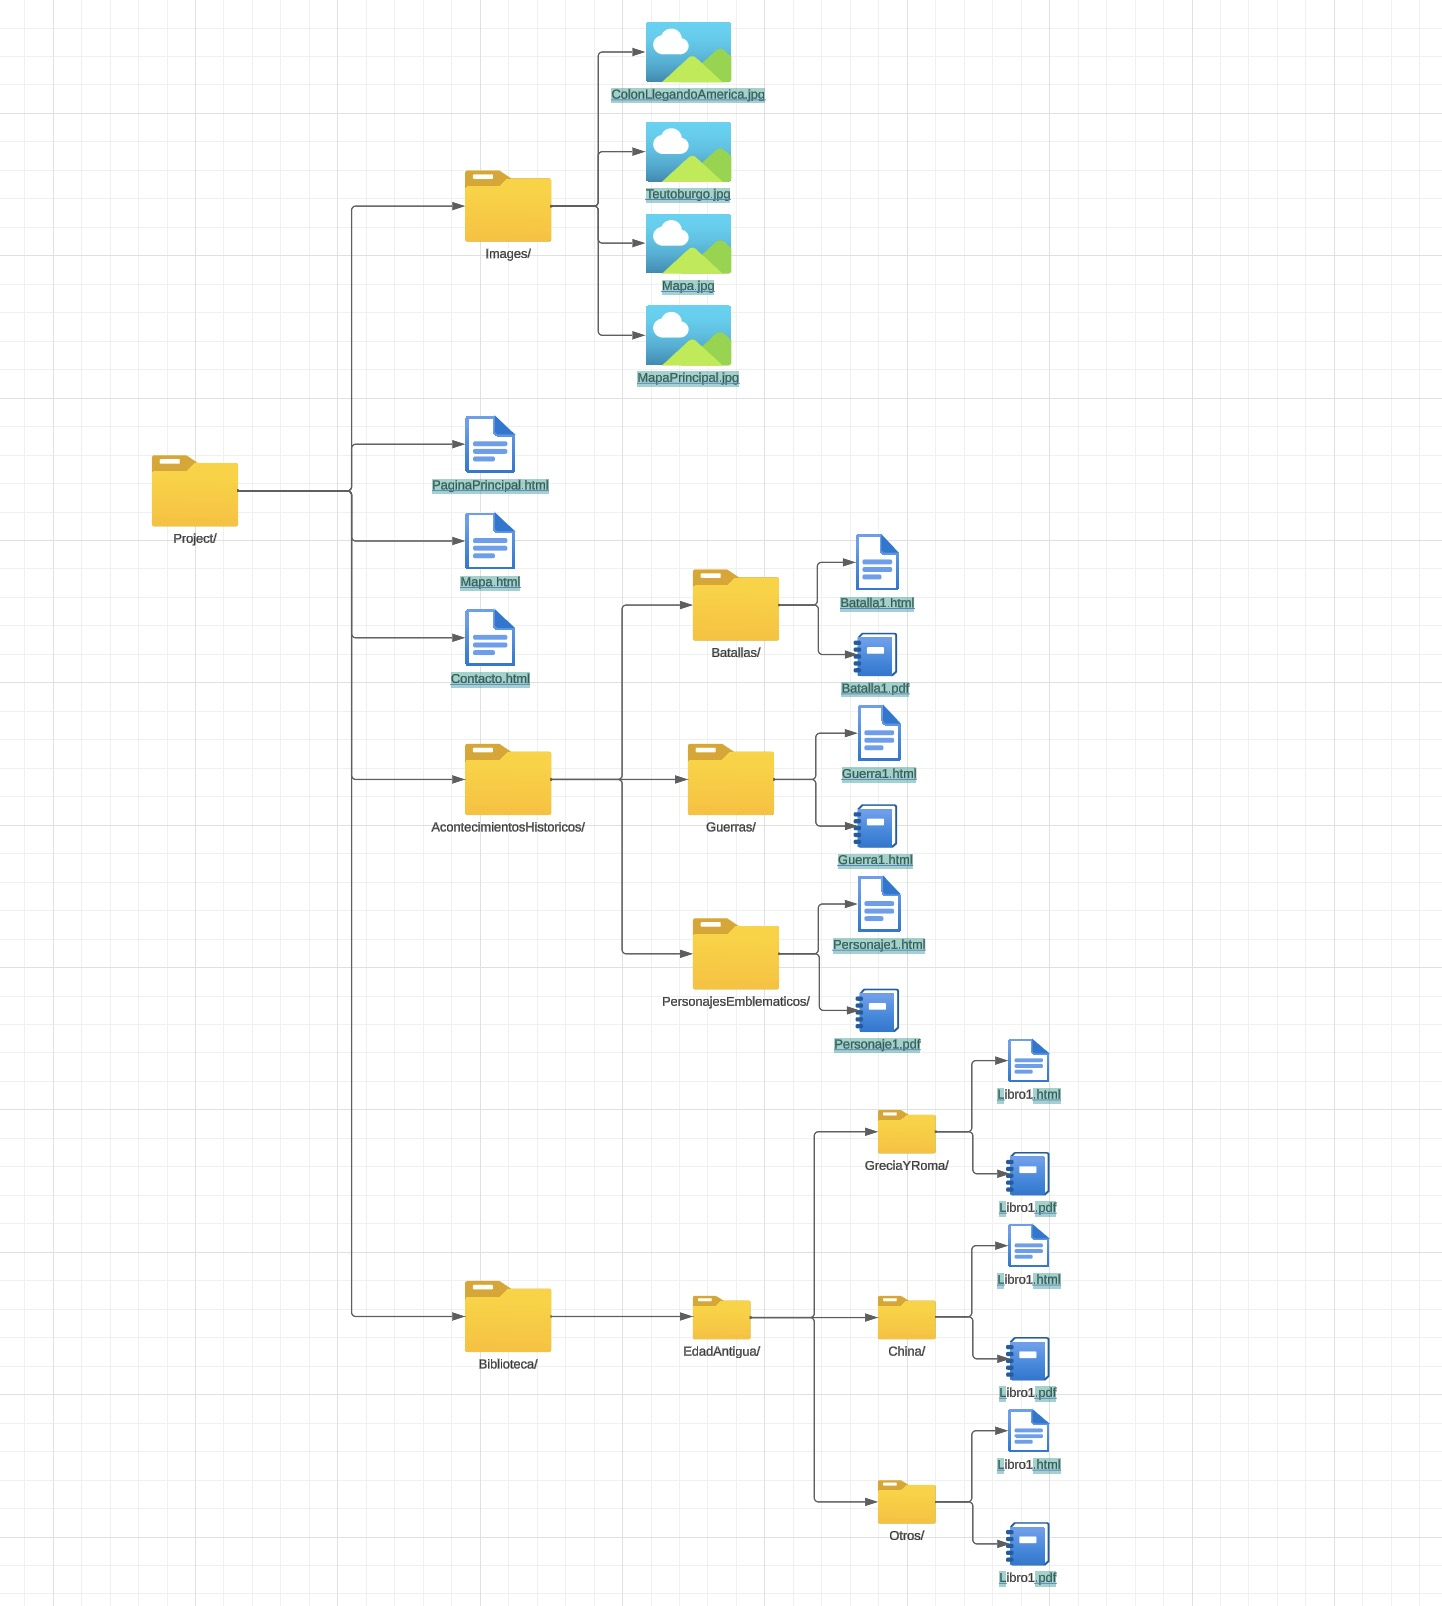
\includegraphics[width=1\textwidth]{Esquemas/EstructuraDeFicheros.jpg}
    \caption{Estructura de Ficheros y Carpetas}
    \label{fig:mi_imagen}
\end{figure}

Este esquema nos proporciona una vista general de como será la estructura que compondrá la página web, siendo extendida en la parte de la biblioteca, donde solo hemos metido una de las carpetas para ilustrar como será para todas ellas.

\newpage

\section{HTML}

Con la evolución del proyecto, las páginas modeladas al comienzo de este también fueron sujetas a cambios, por lo que en esta sección presentamos las páginas HTML finales, de las cinco partes mas significativas de nuestra web.

\subsection{Mapa de etiquetas}

\subsubsection*{index.html}

Esta es la página principal de nuestra web, donde se muestra un mensaje de bienvenida y se da acceso a las distintas secciones de la página.

\begin{figure}[H]
    \centering
    % Primera imagen (izquierda)
    \begin{minipage}{0.49\textwidth}
        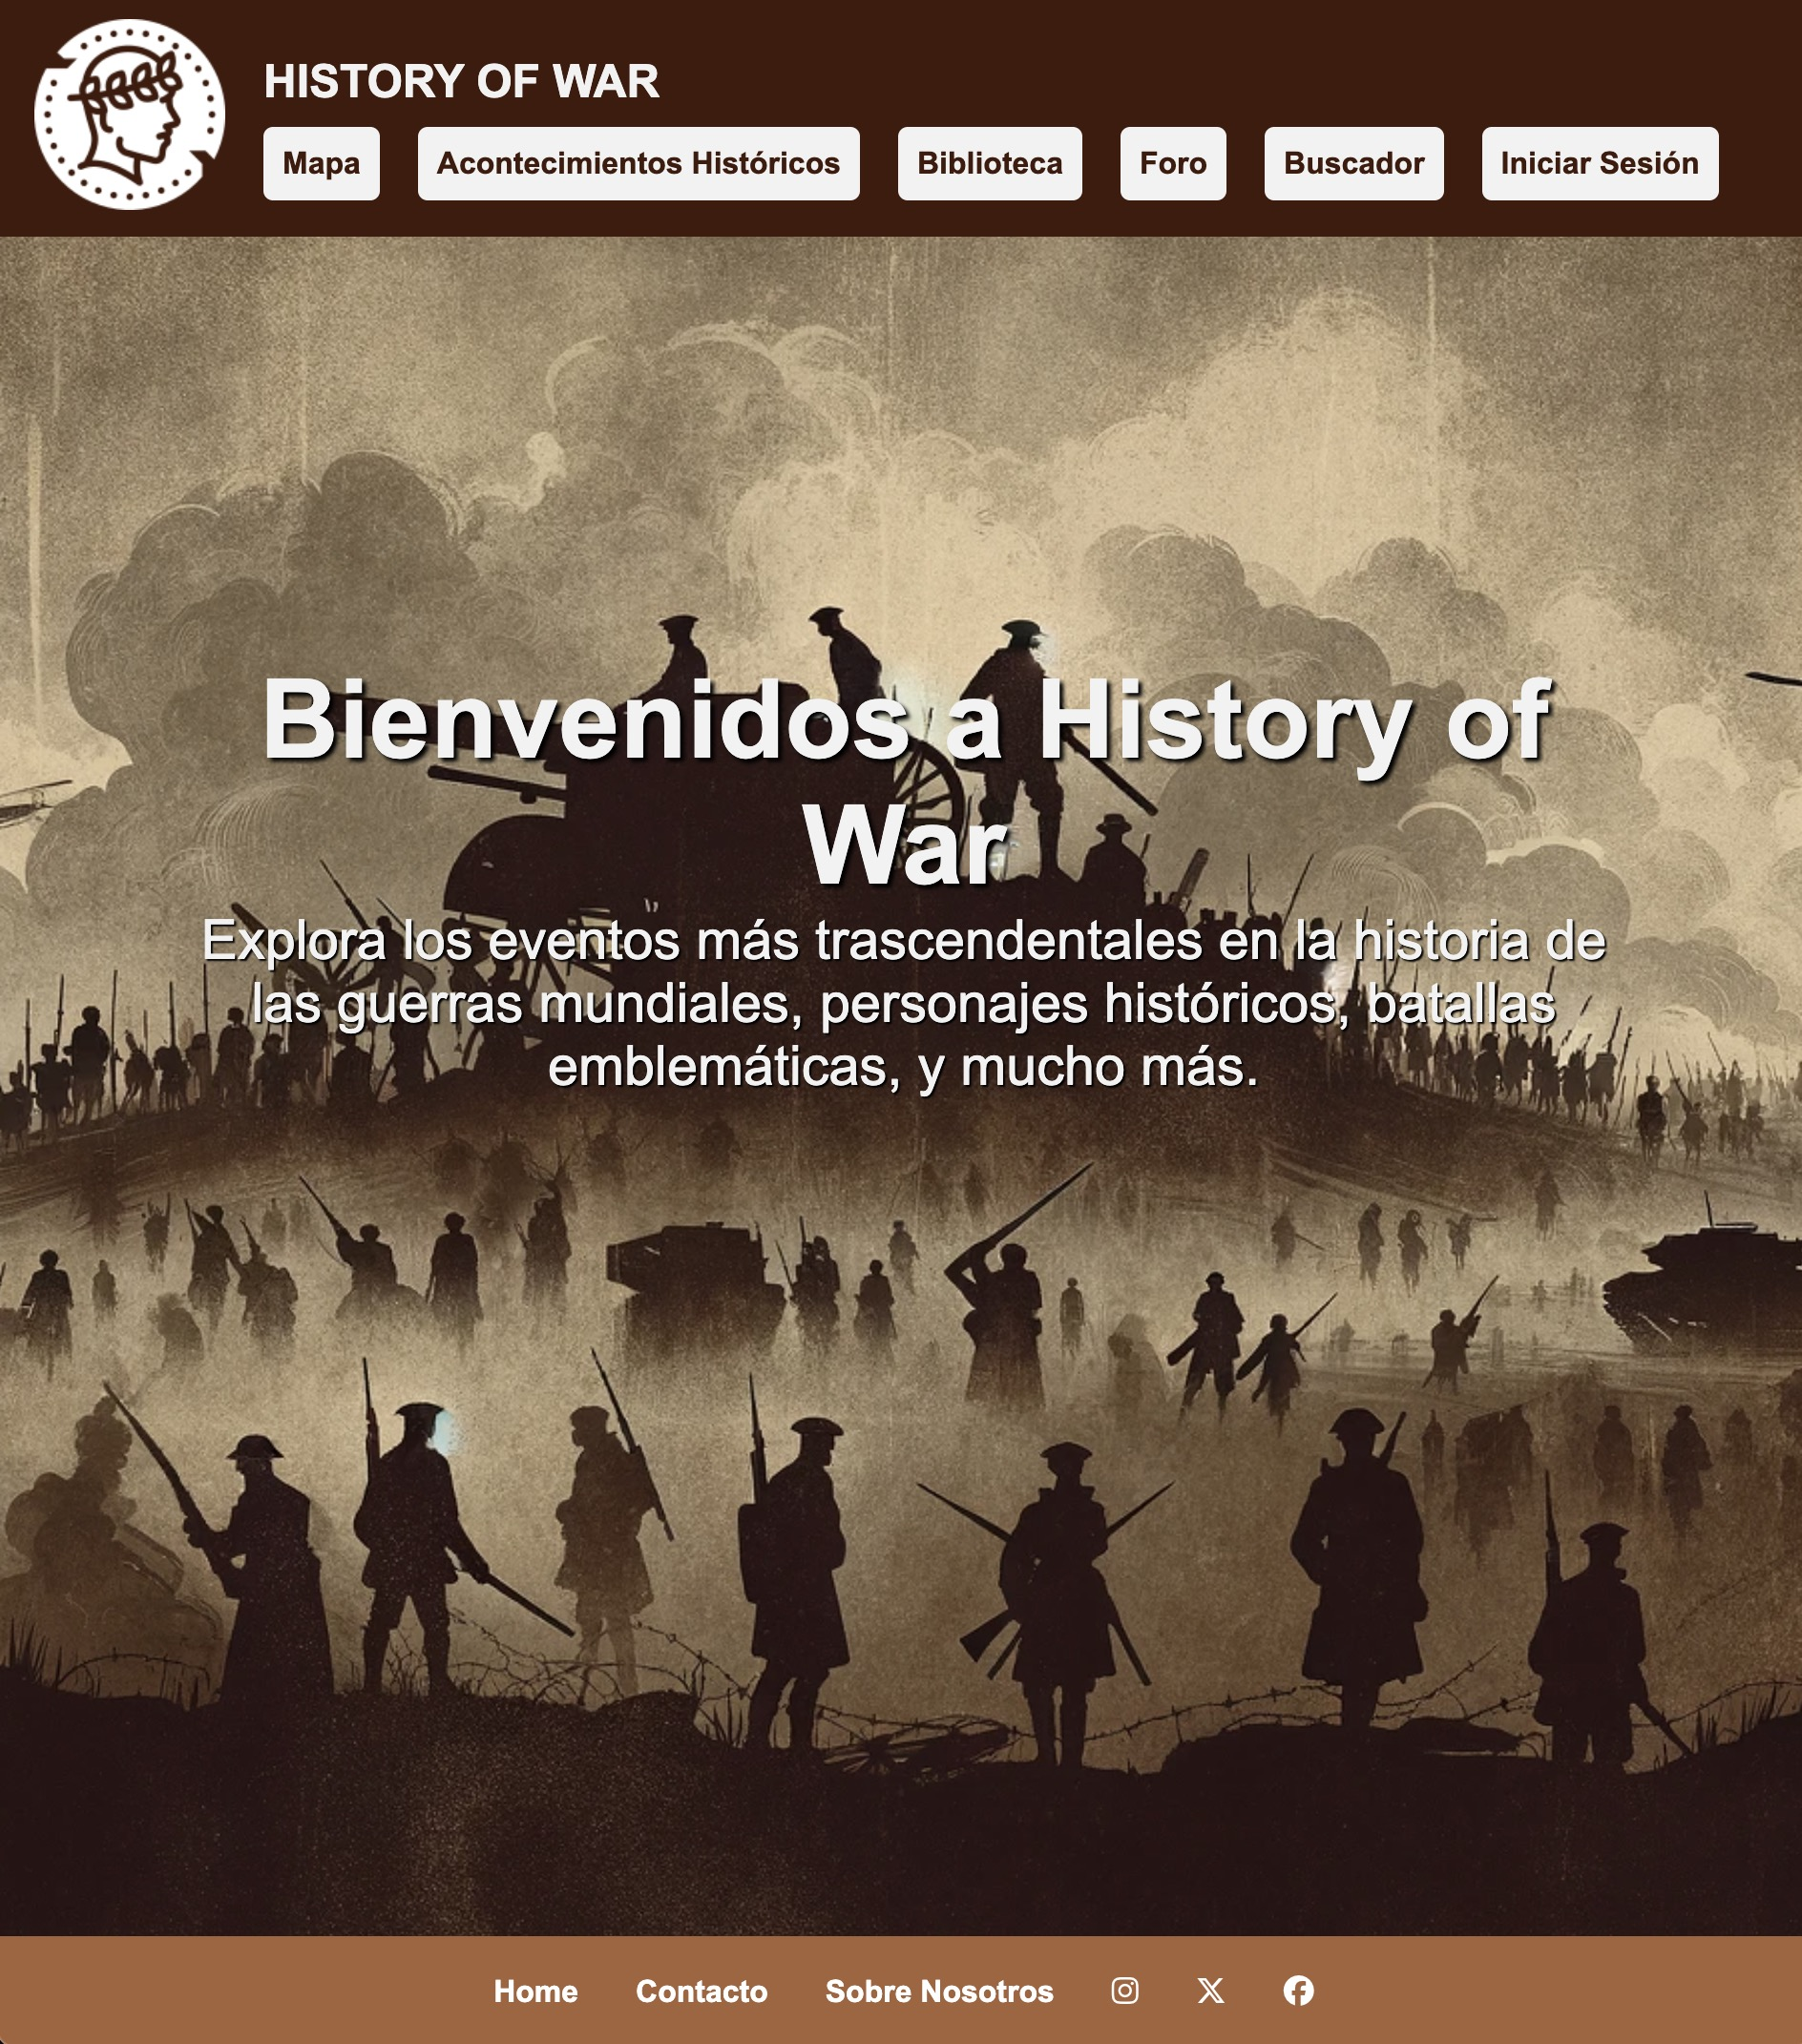
\includegraphics[width=\linewidth]{htmlFotos/pagPrincipal.png}
    \end{minipage}\hfill
    % Segunda imagen (derecha)
    \begin{minipage}{0.49\textwidth}
        \includegraphics[width=\linewidth]{htmlFotos/prototipoPagPrincipal.png}
    \end{minipage}
    
    % Ajuste de espacio vertical si es necesario
    \vspace{5mm}
    
    % Tercera imagen (debajo)
    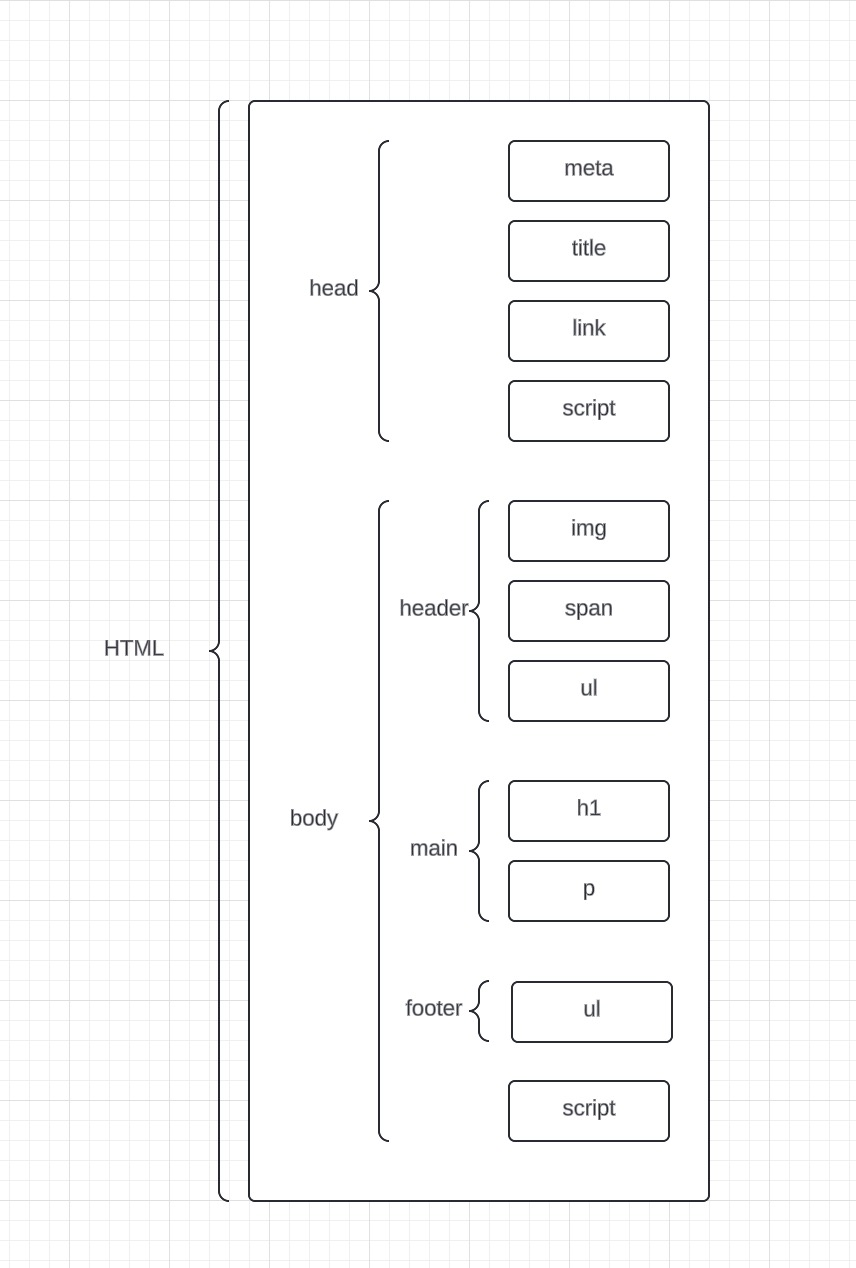
\includegraphics[width=\textwidth, height=0.3\textheight, keepaspectratio]{htmlFotos/MEindex.png}
    \caption{a) Interfaz de index.html b) Prototipo de interfaz de index.html c) Mapa de etiquetas de index.html}
    \label{fig:imagenes_conjuntas}
\end{figure}

\newpage

\subsubsection*{mapa.html}

En esta página se muestra un mapa interactivo que permite al usuario acceder a las distintas batallas de la historia. Para simplificar la visualización, se omite la parte del header y del footer, pues es la msima para todas las páginas.

\begin{figure}[H]
    \centering
    % Primera imagen (izquierda)
    \begin{minipage}{0.49\textwidth}
        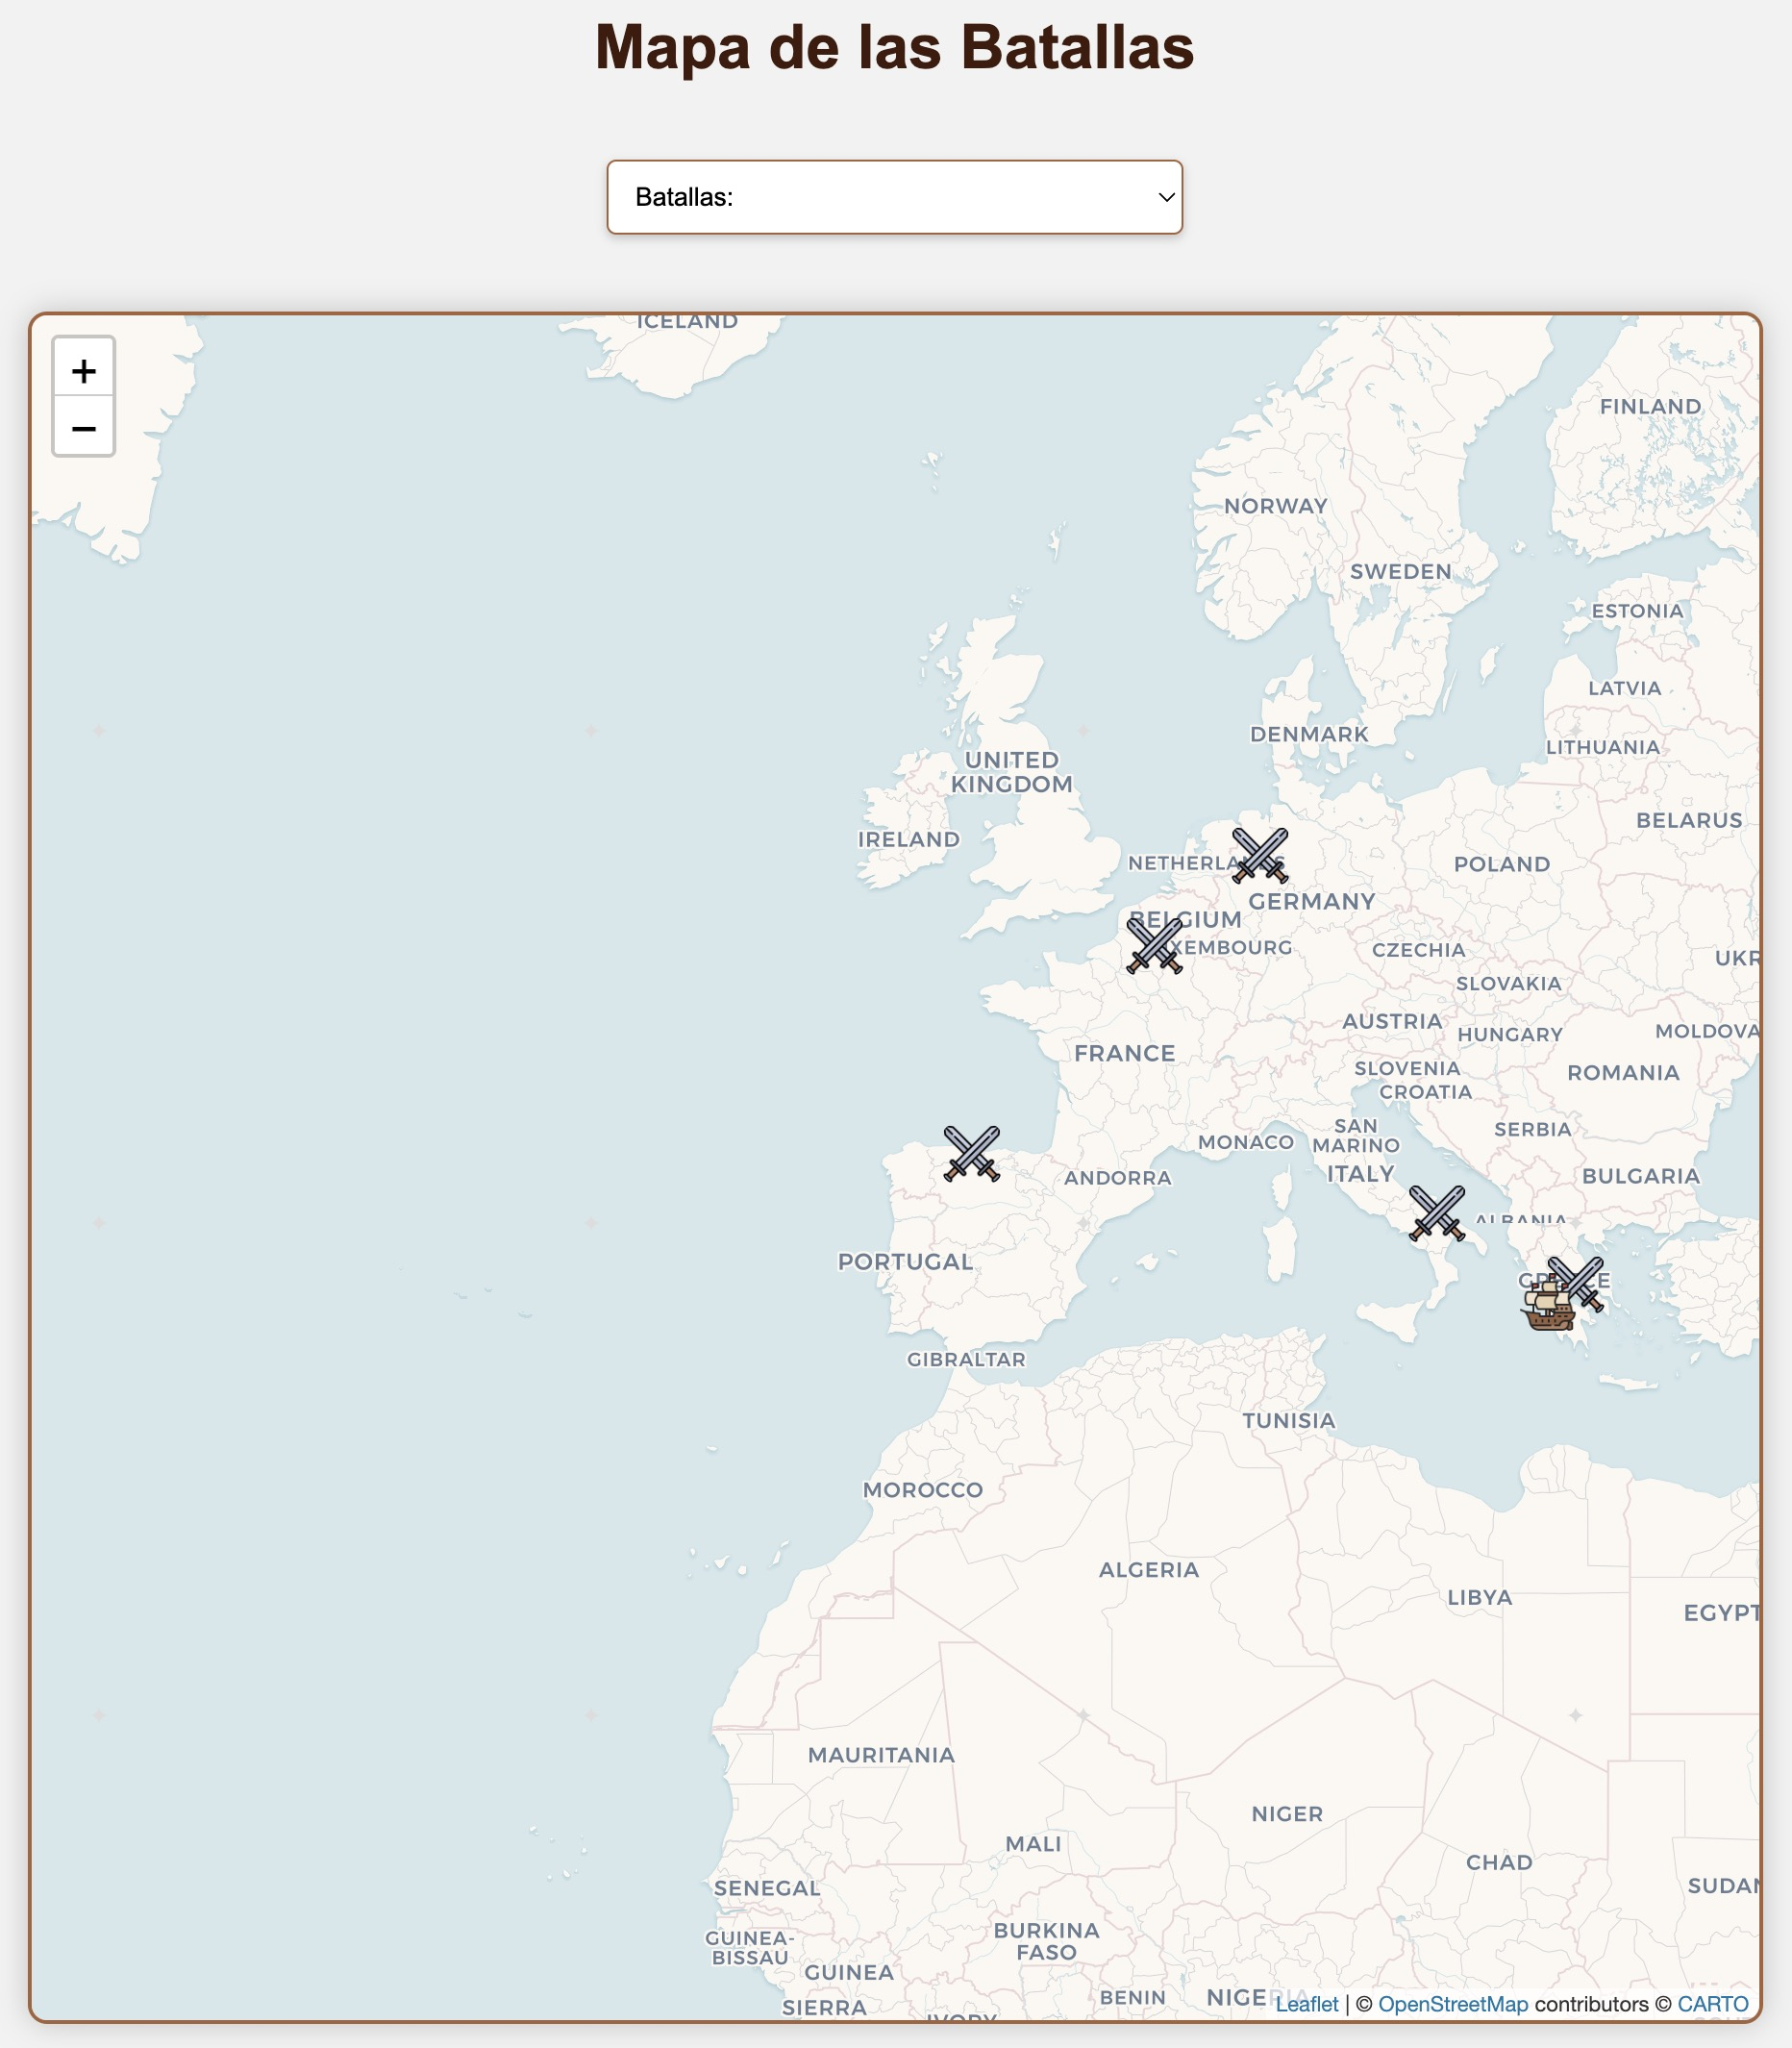
\includegraphics[width=\linewidth]{htmlFotos/mapa.jpg}
    \end{minipage}\hfill
    % Segunda imagen (derecha)
    \begin{minipage}{0.49\textwidth}
        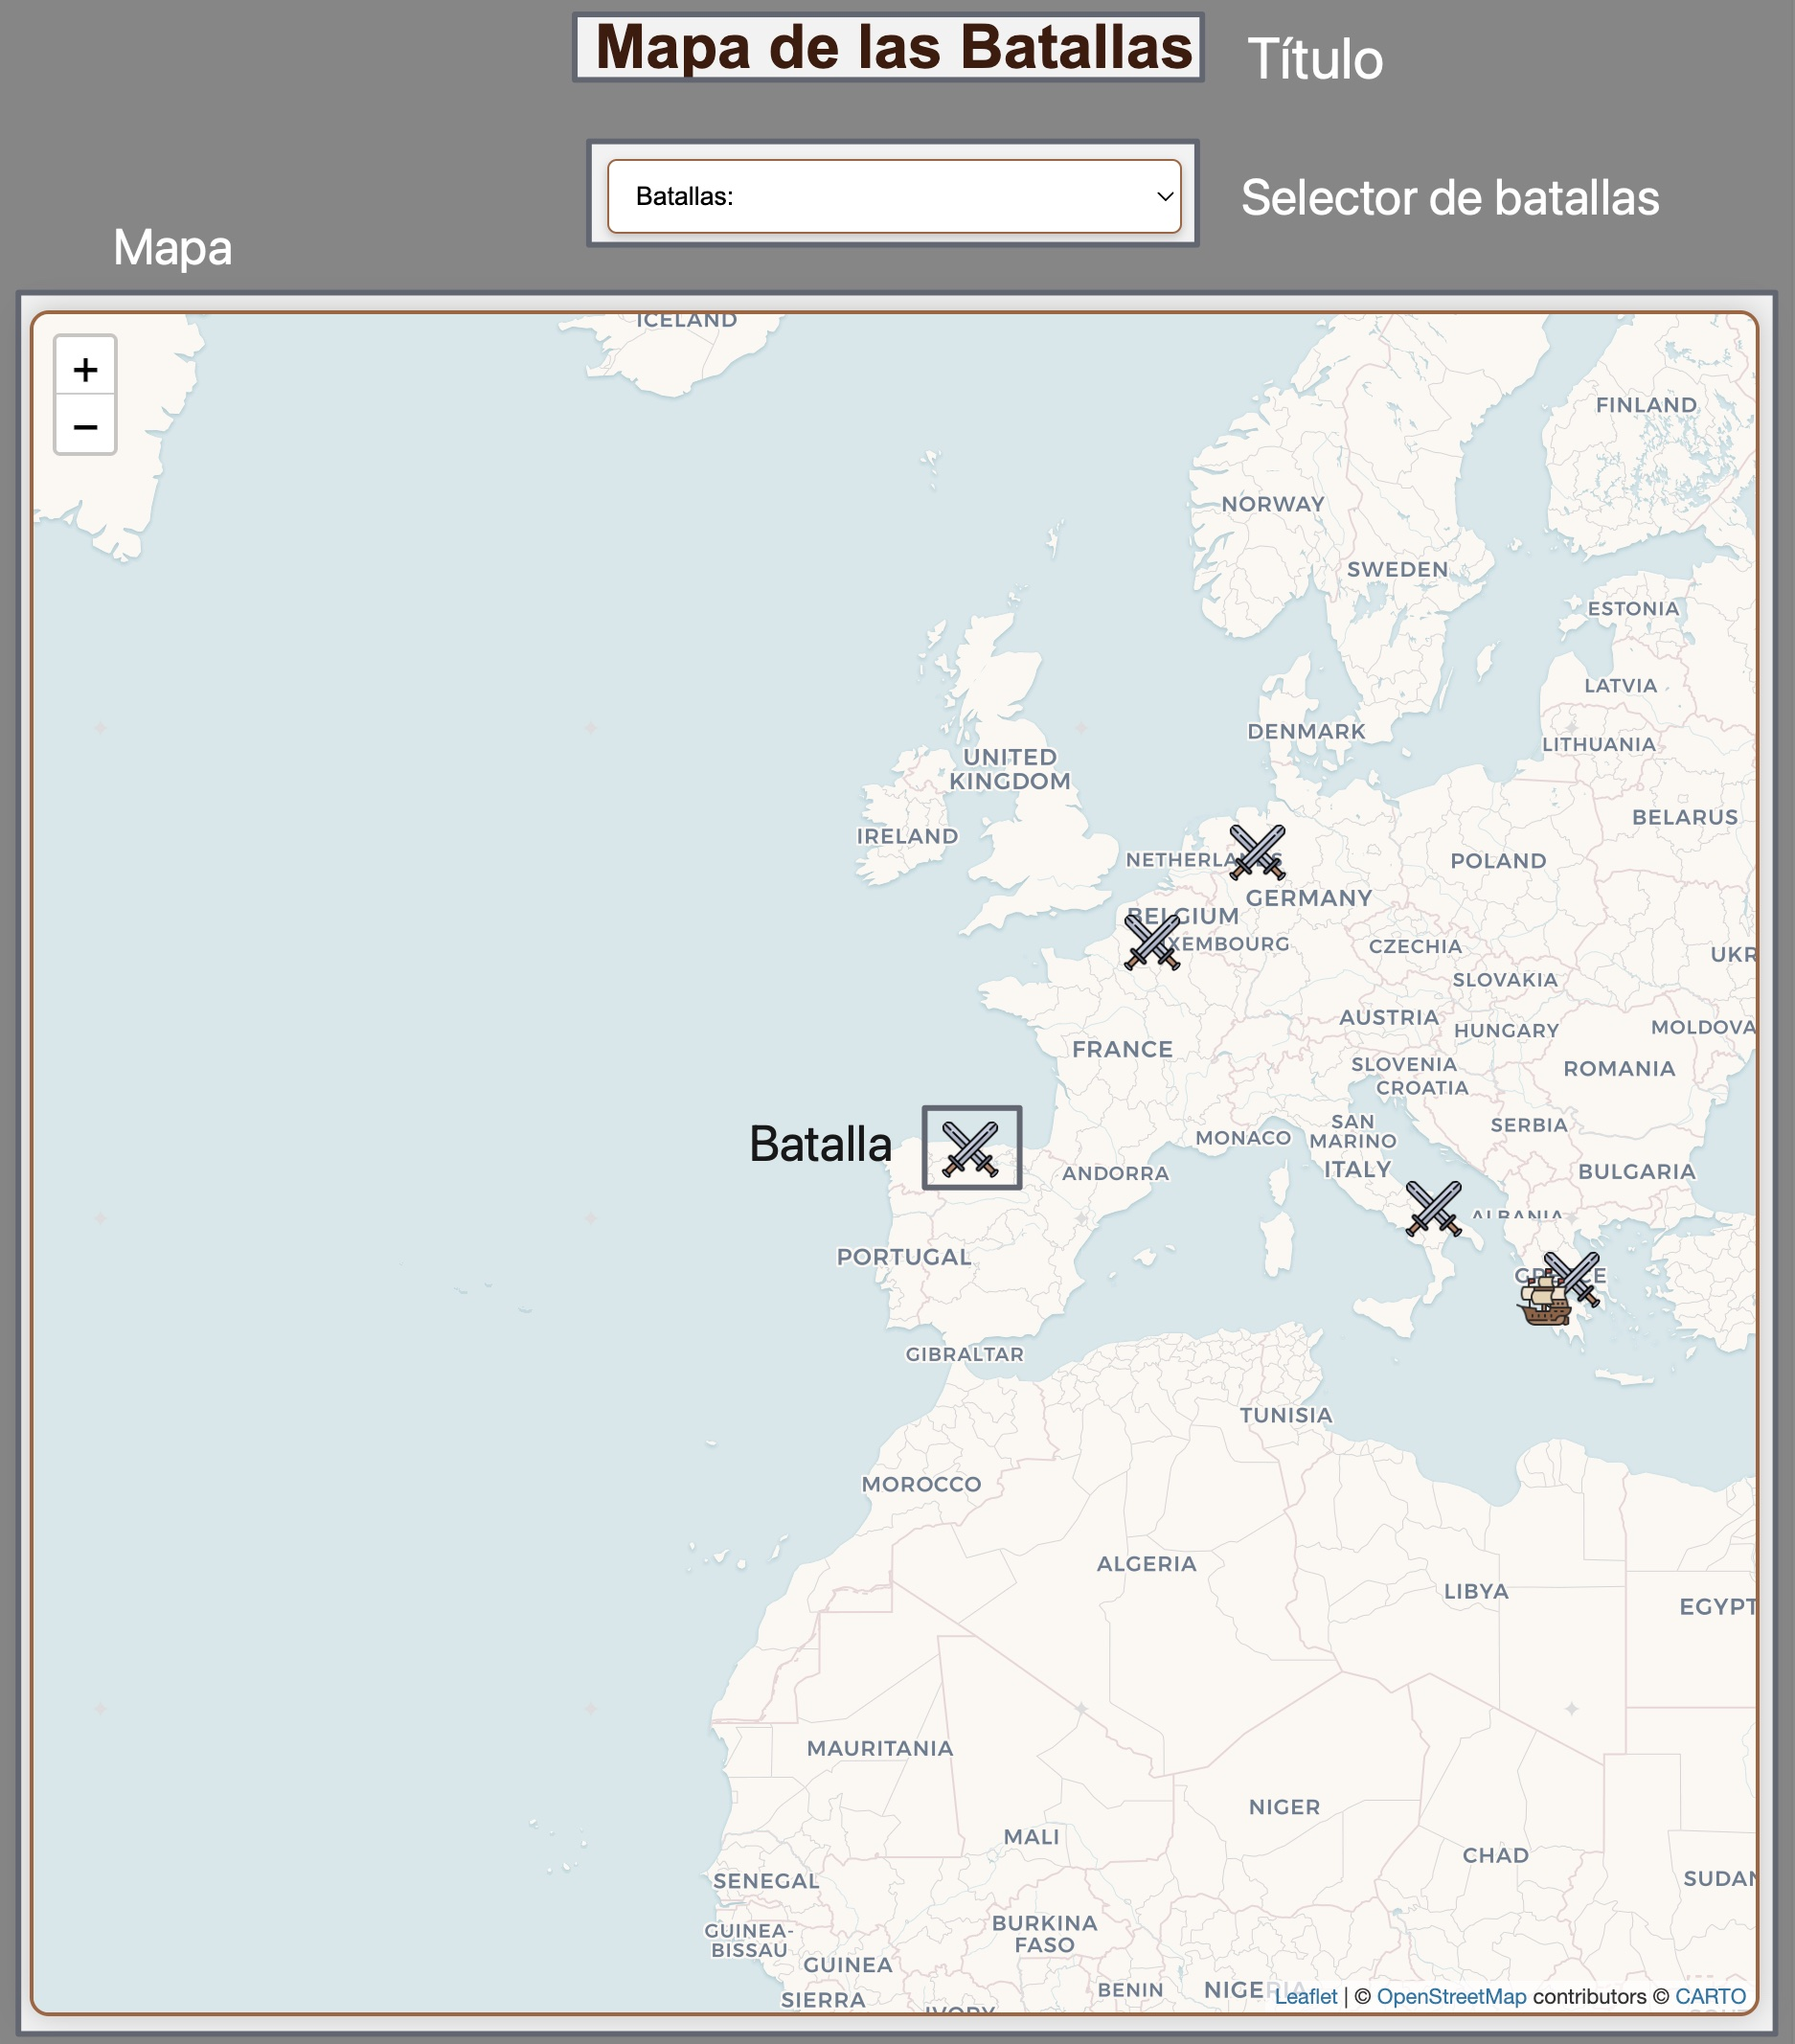
\includegraphics[width=\linewidth]{htmlFotos/prototipoMapa.jpg}
    \end{minipage}
    
    % Ajuste de espacio vertical si es necesario
    \vspace{5mm}
    
    % Tercera imagen (debajo)
    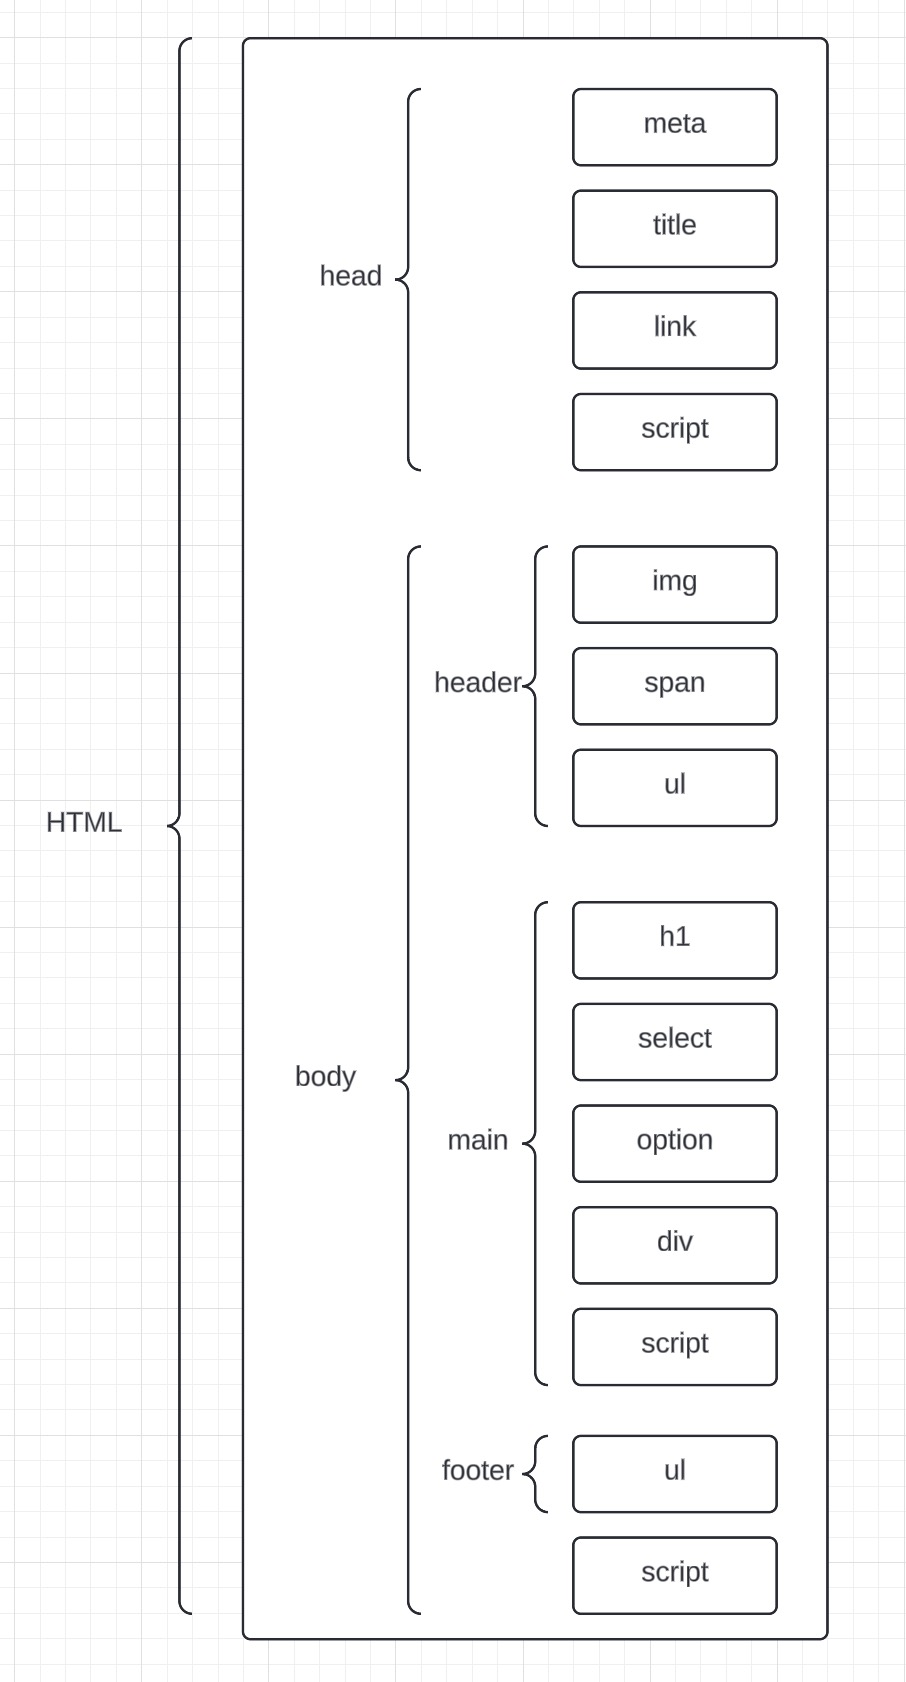
\includegraphics[width=\textwidth, height=0.4\textheight, keepaspectratio]{htmlFotos/MEmapa.jpg}
    \caption{a) Interfaz de AH.html b) Prototipo de interfaz de AH.html c) Mapa de etiquetas de AH.html}
    \label{fig:imagenes_conjuntas}
\end{figure}

\newpage

\subsubsection*{AH.html, batallas.html, guerras.html y personajesEmblematicos.html}

Para ver como se descomponen estas secciones de nuestra web, tomaremos como ejemplo la página de Acontecimientos Históricos, aunque las otras páginas siguen un esquema similar. Como en el caso anterior, se omite la parte del header y del footer, pues es la misma para todas las páginas.

\begin{figure}[H]
    \centering
    % Primera imagen (izquierda)
    \begin{minipage}{0.49\textwidth}
        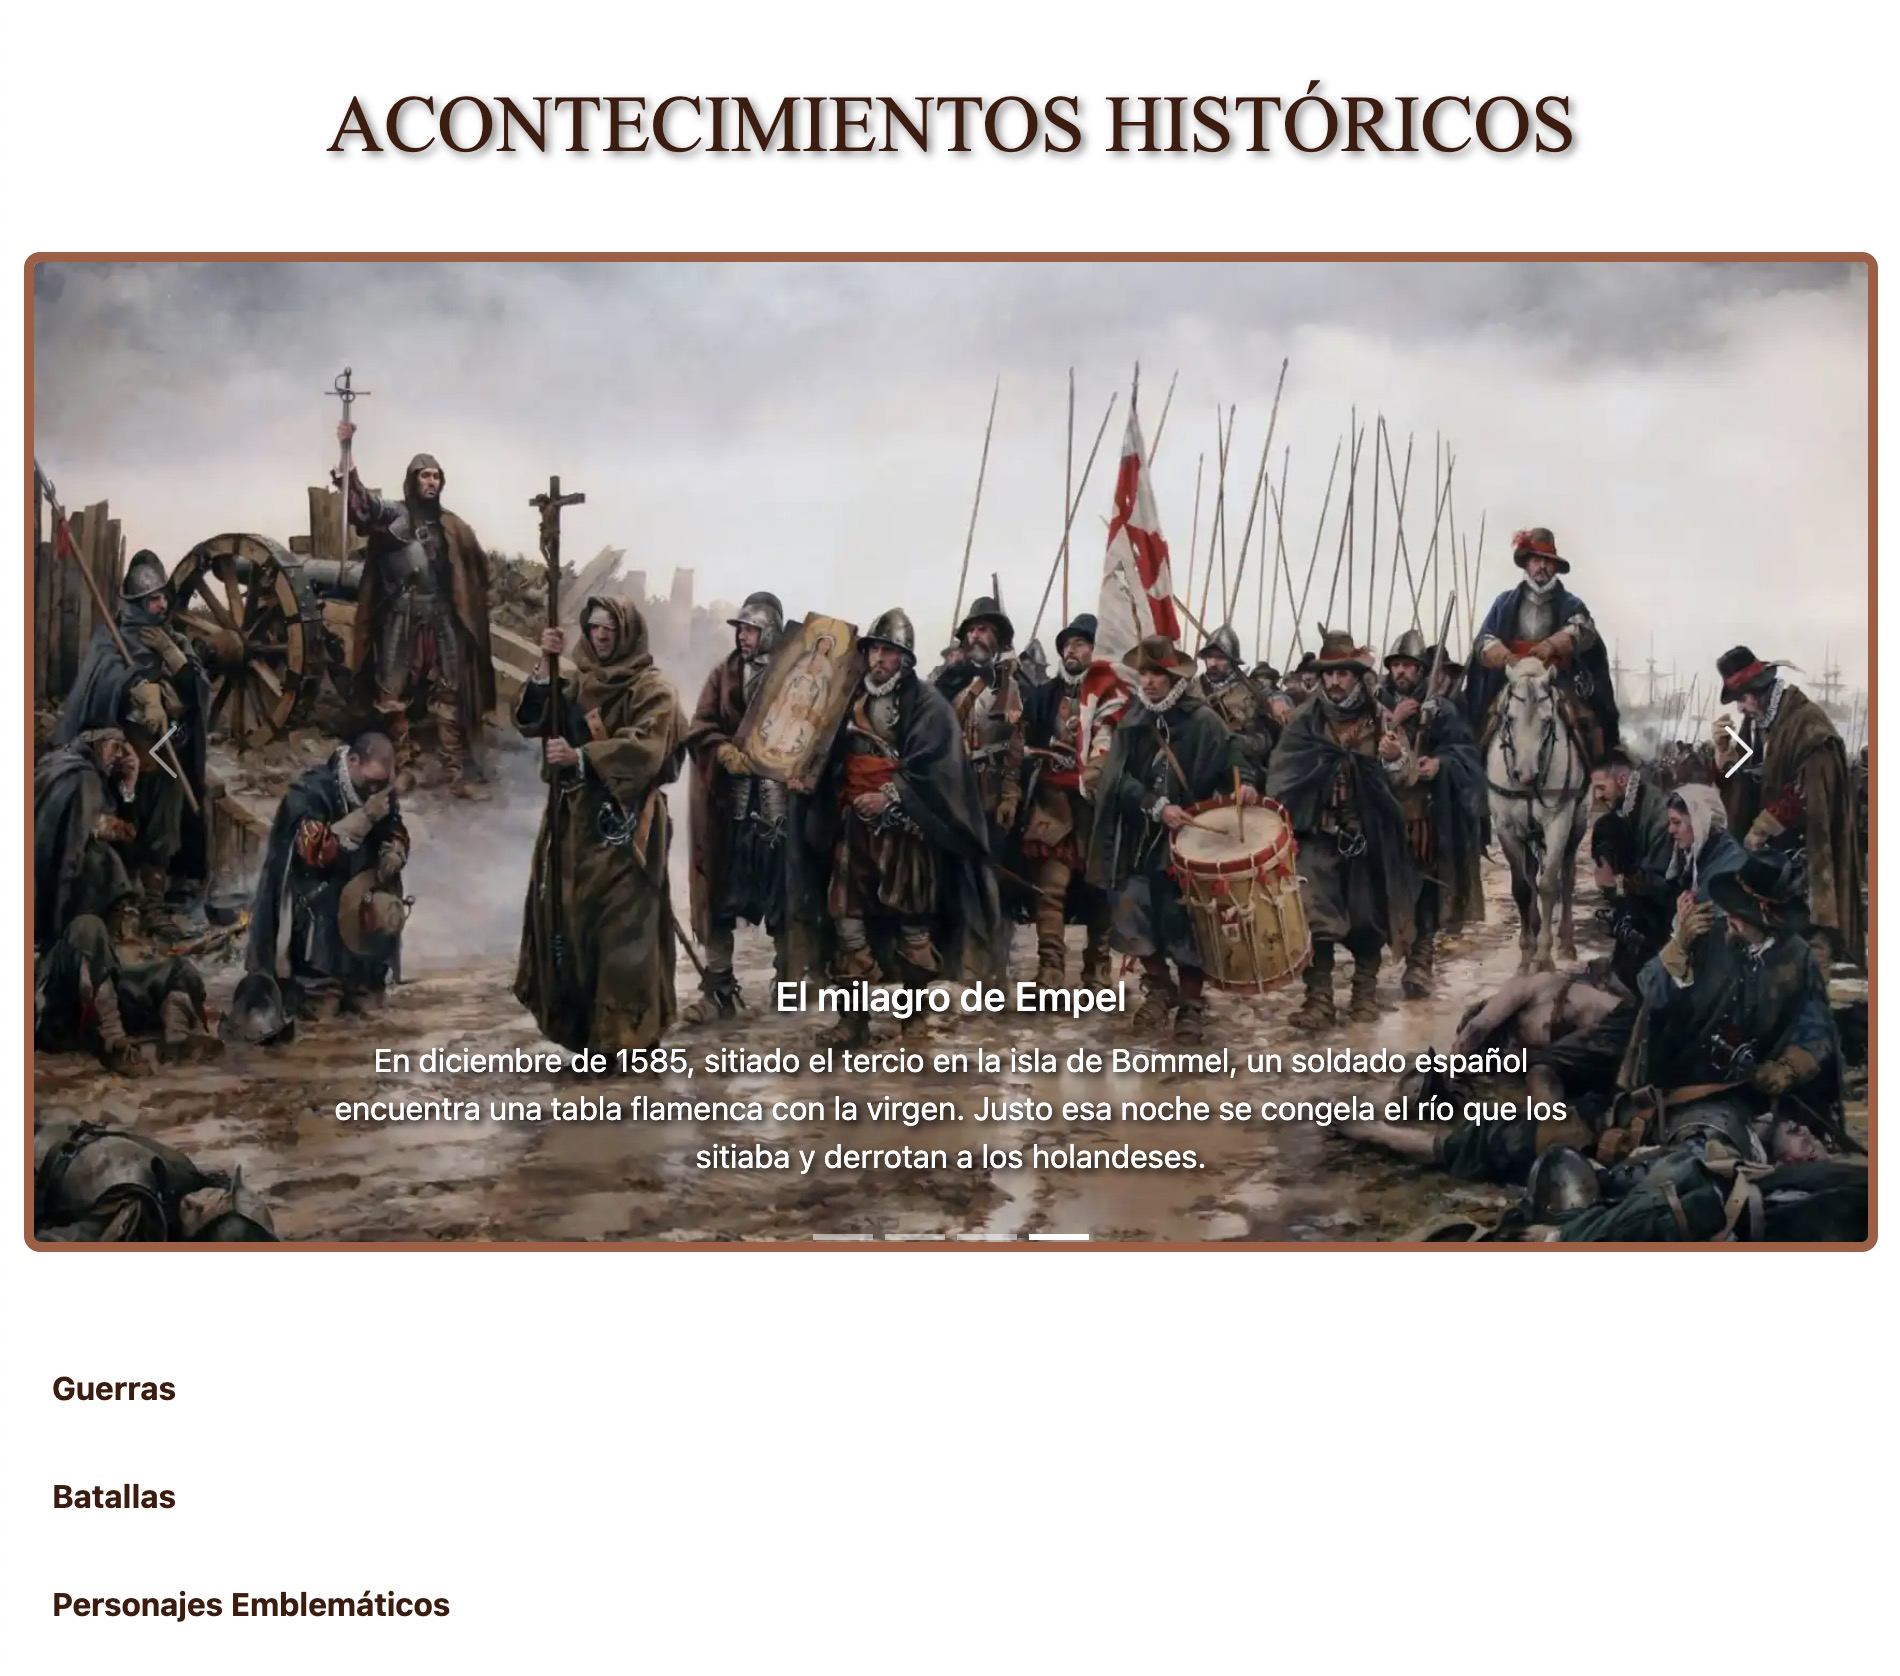
\includegraphics[width=\linewidth]{htmlFotos/AH.jpg}
    \end{minipage}\hfill
    % Segunda imagen (derecha)
    \begin{minipage}{0.49\textwidth}
        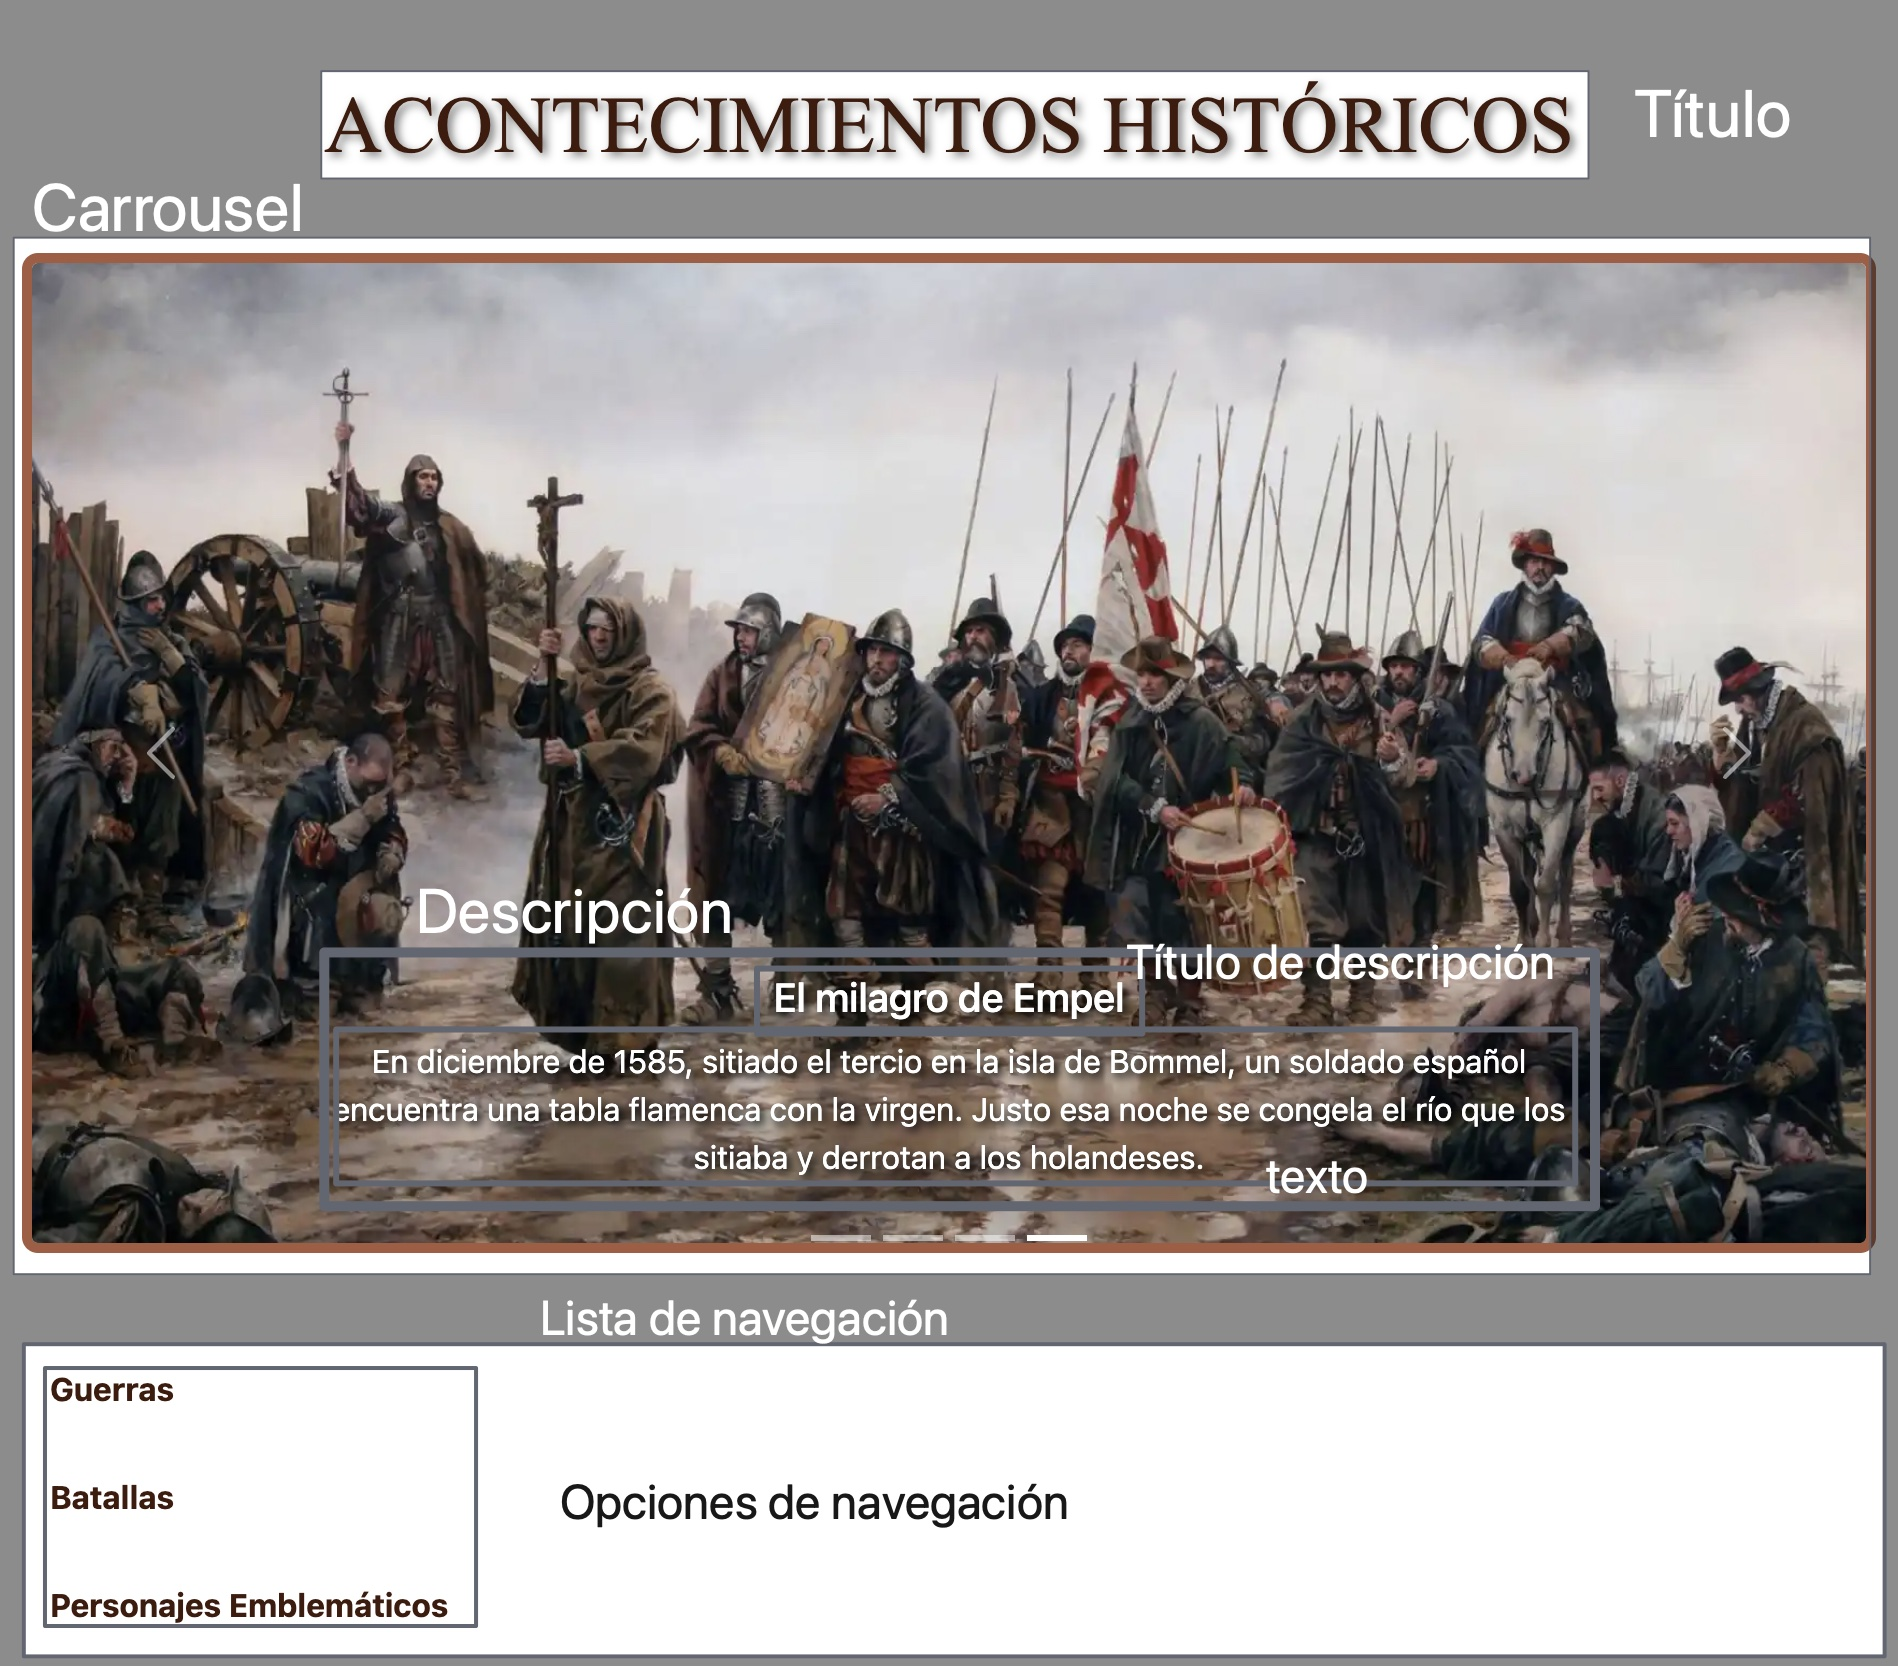
\includegraphics[width=\linewidth]{htmlFotos/prototipoAH.jpg}
    \end{minipage}
    
    % Ajuste de espacio vertical si es necesario
    \vspace{5mm}
    
    % Tercera imagen (debajo)
    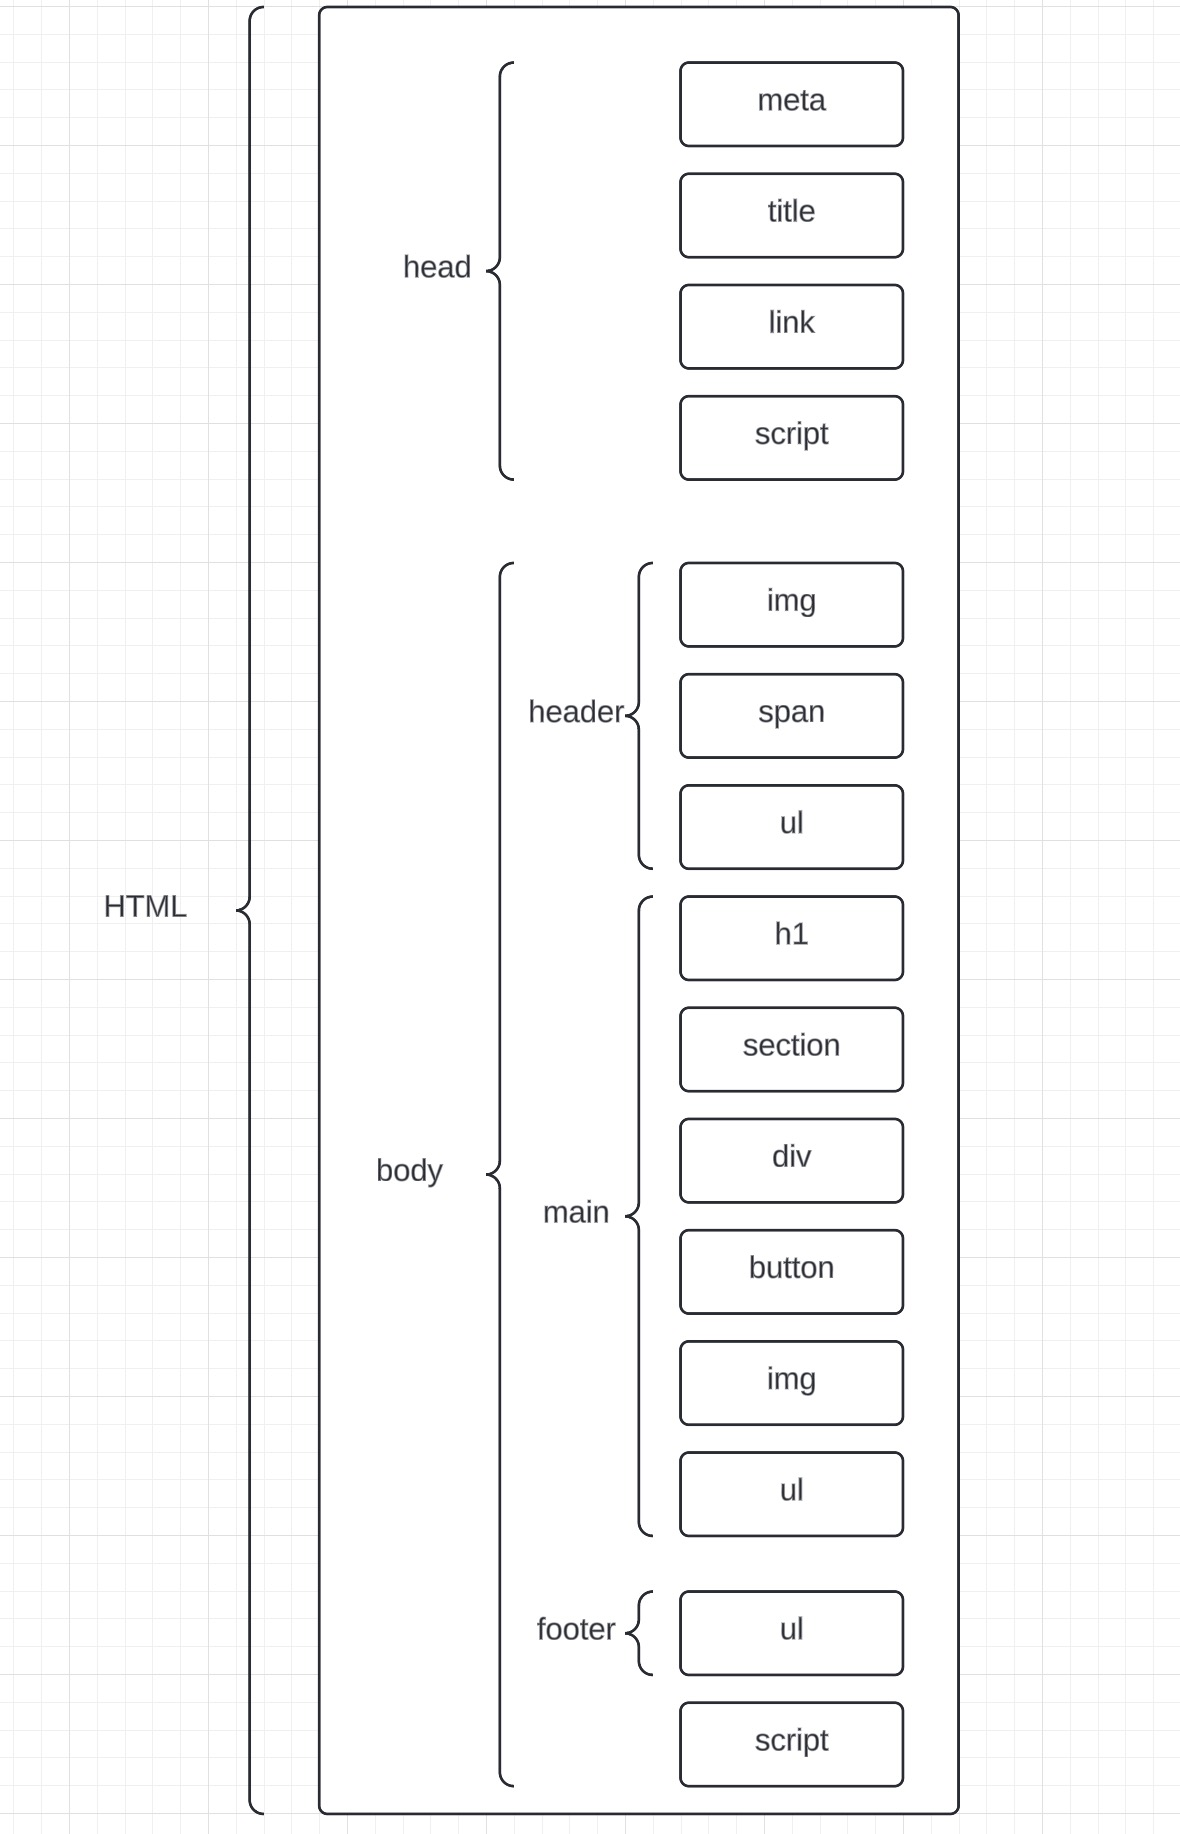
\includegraphics[width=\textwidth, height=0.5\textheight, keepaspectratio]{htmlFotos/MEAH.jpg}
    \caption{a) Interfaz de mapa.html b) Prototipo de interfaz de mapa.html c) Mapa de etiquetas de mapa.html}
    \label{fig:imagenes_conjuntas}
\end{figure}


\end{document}
